\documentclass{article}

\usepackage{graphicx}
\usepackage[utf8]{inputenc}
\usepackage{amsmath}
\usepackage{listings}

\graphicspath{{artifact/images/}}
\numberwithin{equation}{section}
\numberwithin{figure}{section}
\numberwithin{table}{section}
\newtheorem{theorem}{Theorem}[section]
\newtheorem{proposition}{Proposition}[section]
\newtheorem{definition}[theorem]{Definition}

\begin{document}

\title{Converting Graphic Relationships into Conditional Probabilities in Bayesian Network}

\author{
Loc Nguyen\\
Sunflower Soft Company, An Giang, Vietnam\\
ng\_phloc@yahoo.com
}

\maketitle

\begin{abstract}
Bayesian network is a powerful mathematical tool for prediction and diagnosis applications. A large Bayesian network can be constituted of many simple networks which in turn are constructed from simple graphs. A simple graph consists of one child node and many parent nodes. The strength of each relationship between a child node and a parent node is quantified by a weight and all relationships share the same semantics such as prerequisite, diagnostic, and aggregation. The research focuses on converting graphic relationships into conditional probabilities in order to construct a simple Bayesian network from a graph. Diagnostic relationship is the main research object, in which sufficient diagnostic proposition is proposed for validating diagnostic relationship. Relationship conversion is adhered to logic gates such as AND, OR, and XOR, which is essential feature of the research.

\textit{Keywords}: diagnostic relationship, Bayesian network, transformation coefficient
\end{abstract}

\section{Introduction}
Bayesian network (BN) is a directed acyclic graph (DAG) consisting of a set of nodes and a set of arcs. Each node is a random variable. Each arc represents a relationship between two nodes. The strength of relationship in a graph can be quantified by a number called \textit{weight}. There are some important relationships such as prerequisite, diagnostic, and aggregation. The difference between BN and normal graph is that the strength of every relationship in BN is represented by a conditional probability table (CPT) whose entries are conditional probabilities of a child node given parent nodes. There are two main approaches to construct a BN:

\begin{enumerate}
\item  The first approach aims to learn BN from training data by learning machine algorithms.

\item  The second approach is that experts define some graph patterns according to specific relationships and then, BN is constructed based on such patterns along with determined CPT (s).
\end{enumerate}

This research focuses on the second approach in which relationships are converted into CPT (s). Essentially, relationship conversion aims to determined conditional probabilities based on weights and meanings of relationships. We will have different ways to convert graphic weights into CPT (s) for different relationships. It is impossible to convert all relationships but some of them such as diagnostic, aggregation, and prerequisite are mandatory ones that we must specify as computable CPT (s) of BN. Especially, these relationships are adhered to logic X-gates \cite{wikipedia:logic-gates} such as AND-gate, OR-gate, and SIGMA-gate. The X-gate inference in this research is derived and inspired from noisy OR-gate described in the book ``Learning Bayesian Networks'' by author \cite[pp.~157-159]{neapolitan:bn}. Authors \cite{diez:pmodels} also researched OR/MAX, AND/MIN, noisy XOR inferences but they focused on canonical models, deterministic models, ICI models whereas I focus on logic gate and graphic relationships. So their research is different from mine but we share the same result that is AND-gate model. In general, my research focuses on applied probability adhered to Bayesian network, logic gates, and Bayesian user modeling \cite{millan:bayesiandiagnostic}. The scientific results are shared with authors Eva Millán and José Luis Pérez-de-la-Cruz \cite{millan:bayesiandiagnostic}.

Factor graph \cite{wikipedia:factor-graph} represents factorization of a global function into many partial functions. If joint distribution of BN is considered as the global function and CPT (s) are considered as partial functions, the sum-product algorithm \cite{kschischang:factor-graph} of factor graph is applied into calculating posterior probabilities of variables in BN. Pearl's propagation algorithm \cite{pearl:propagation} is very successful in BN inference. The application of factor graph into BN is only realized if all CPT (s) of BN are already determined whereas this research focuses on defining such CPT (s) firstly. I did not use factor graph for constructing BN. The concept ``X-gate inference'' only implies how to convert simple graph into BN. However the arrange sum with a fixed variable mentioned in this research is the ``not-sum'' \cite[p.~499]{kschischang:factor-graph} of factor graph. Essentially, X-gate probability shown in formula~\ref{formula:x-gate-prob} is as same as $\lambda$ message in the Pearl's algorithm \cite[p.~518]{kschischang:factor-graph} but I use the most basic way to prove the X-gate probability.

As default, the research is applied in learning context in which BN is used to assess students' knowledge. Evidences are tests, exams, exercises, etc. and hypotheses are learning concepts, knowledge items, etc. Note that diagnostic relationship is very important to Bayesian evaluation in learning context because it is used to evaluate student's mastery of concepts (knowledge items) over entire BN. As a convention, all equations are called formulas having particular titles. Now we start relationship conversion with a research on diagnostic relationship in the next section.

\section{Diagnostic relationship}
In some opinions like mine, the diagnostic relationship should be from hypothesis to evidence. For example, disease is hypothesis and symptom is evidence. The symptom must be conditionally dependent on disease. Given a symptom, calculating the posterior probability of disease is essentially to diagnose likelihood of such disease \cite[p.~1666]{millan:bayesiannetwork}. Inversely, the arc from evidence to hypothesis implies prediction where evidence and hypothesis represent observation and event, respectively. Given an observation, calculating the posterior probability of the event is essentially to predict/assert such event \cite[p.~1666]{millan:bayesiannetwork}. Figure~\ref{figure:diagnosis-prediction} shows diagnosis and prediction.

\begin{figure}
\centering
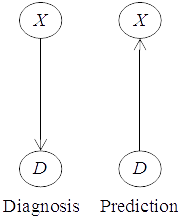
\includegraphics{DiagnosisPrediction.png}
\caption{Diagnosis and prediction with hypothesis \textit{X} and evidence \textit{D}}
\label{figure:diagnosis-prediction}
\end{figure}
%Figure 2.1. Diagnosis and prediction with hypothesis \textit{X} and evidence \textit{D}

The weight \textit{w} of relationship between \textit{X} and \textit{D} is 1. Figure~\ref{figure:diagnosis-prediction} depicts simplest graph with two random variables. We need to convert diagnostic relationship into conditional probabilities in order to construct a simplest BN from the simplest graph. Note that hypothesis is binary but evidence can be numerical. In learning context, evidence \textit{D} can be test, exam, exercise, etc. The conditional probability of \textit{D} given \textit{X} (likelihood function) is \textit{P}(\textit{D}{\textbar}\textit{X}). The posterior probability of \textit{X} is \textit{P}(\textit{X}{\textbar}\textit{D}), which is used to evaluate student's mastery over concept (hypothesis) \textit{X} given evidence \textit{D}. Formula~\ref{formula:cpt-evidence-diagnostic} specifies CPT of \textit{D} when \textit{D} is binary (0 and 1):

\begin{equation}
P\left(D\mathrel{\left|\vphantom{D X}\right.\kern-\nulldelimiterspace}X\right)=\left\{ \begin{array}{r}
D\ \mathrm{if}\ X=1 \\ 
1-D\ \mathrm{if}\ X=0 \end{array}
\right.
\label{formula:cpt-evidence-diagnostic}
\end{equation}
%Formula 2.1. CPT of binary evidence of diagnostic relationship

Formula~\ref{formula:cpt-evidence-diagnostic} is our first relationship conversion. It implies
\[P\left(D\mathrel{\left|\vphantom{D X=0}\right.\kern-\nulldelimiterspace}X=0\right)+P\left(D\mathrel{\left|\vphantom{D X=1}\right.\kern-\nulldelimiterspace}X=1\right)=D+1-D=1\] 
Evidence \textit{D} can be used to diagnose hypothesis \textit{X} if the so-called \textit{sufficient} \textit{diagnostic proposition} is satisfied, as seen in proposition~\ref{proposition:diagnostic-proposition}.

\begin{proposition}[Sufficient diagnostic proposition]
\textit{D} is equivalent to \textit{X} in diagnostic relationship if \textit{P}(\textit{X}{\textbar}\textit{D}) = \textit{kP}(\textit{D}{\textbar}\textit{X}) given uniform distribution of \textit{X} and the \textit{transformation coefficient k} is independent from \textit{D}. In other words, \textit{k} is constant with regards to \textit{D }and\textit{ }so \textit{D} is called \textit{sufficient evidence}.
\label{proposition:diagnostic-proposition}
\end{proposition}
%Table 2.1. Sufficient diagnostic proposition

The concept of sufficient evidence is borrowed from the concept of sufficient statistics and it is inspired from equivalence of variables \textit{T} and \textit{T'} in the research \cite[pp.~292-295]{millan:bayesiandiagnostic}. The proposition can be restated that evidence \textit{D} is only used to assess hypotheses if it is sufficient evidence. As a convention, the proposition is called \textit{diagnostic condition} and hypotheses have uniform distribution. The assumption of hypothetic uniform distribution (\textit{P}(\textit{X}=1) = \textit{P}(\textit{X}=0)) implies that we cannot assert whether or not given hypothesis is true before we observe its evidence.

In learning context, \textit{D} can be totally used to assess student's mastery of \textit{X} if diagnostic condition is satisfied. Derived from such condition, formula~\ref{formula:transformation-coefficient} specifies transformation coefficient \textit{k} given uniform distribution of \textit{X}.

\begin{equation}
k=\frac{P\left(X\mathrel{\left|\vphantom{X D}\right.\kern-\nulldelimiterspace}D\right)}{P\left(D\mathrel{\left|\vphantom{D X}\right.\kern-\nulldelimiterspace}X\right)} 
\label{formula:transformation-coefficient}
\end{equation}
%Formula 2.2. Transformation coefficient given uniform distribution of \textit{X}

We need to prove that formula~\ref{formula:cpt-evidence-diagnostic} satisfies diagnostic condition. Suppose the prior probability of \textit{X} is uniform:
\[P\left(X=0\right)=P\left(X=1\right)\] 
We have:
\begin{align*}
&P\left(X\mathrel{\left|\vphantom{X D}\right.\kern-\nulldelimiterspace}D\right)=\frac{P\left(D\mathrel{\left|\vphantom{D X}\right.\kern-\nulldelimiterspace}X\right)P\left(X\right)}{P\left(D\right)}\\
&=\frac{P\left(D\mathrel{\left|\vphantom{D X}\right.\kern-\nulldelimiterspace}X\right)P\left(X\right)}{P\left(D\mathrel{\left|\vphantom{D X=0}\right.\kern-\nulldelimiterspace}X=0\right)P\left(X=0\right)+P\left(D\mathrel{\left|\vphantom{D X=1}\right.\kern-\nulldelimiterspace}X=1\right)P\left(X=1\right)}\\
&\left(\mathrm{due\ to\ Baye}{\mathrm{s}}^{\mathrm{'}}\mathrm{rule}\right)\\
&=\frac{P\left(D\mathrel{\left|\vphantom{D X}\right.\kern-\nulldelimiterspace}X\right)P\left(X\right)}{P\left(X\right)\left(P\left(D\mathrel{\left|\vphantom{D X=0}\right.\kern-\nulldelimiterspace}X=0\right)+P\left(D\mathrel{\left|\vphantom{D X=1}\right.\kern-\nulldelimiterspace}X=1\right)\right)}\\
&\left(\mathrm{due\ to}\ P\left(X=0\right)=P\left(X=1\right)\right)\\
&=\frac{P\left(D\mathrel{\left|\vphantom{D X}\right.\kern-\nulldelimiterspace}X\right)}{P\left(D\mathrel{\left|\vphantom{D X=0}\right.\kern-\nulldelimiterspace}X=0\right)+P\left(D\mathrel{\left|\vphantom{D X=1}\right.\kern-\nulldelimiterspace}X=1\right)}=1*P\left(D\mathrel{\left|\vphantom{D X}\right.\kern-\nulldelimiterspace}X\right)\\
&\left(\mathrm{due\ to}\ P\left(D\mathrel{\left|\vphantom{D X=0}\right.\kern-\nulldelimiterspace}X=0\right)+P\left(D\mathrel{\left|\vphantom{D X=1}\right.\kern-\nulldelimiterspace}X=1\right)=1\right)
\end{align*}
It is easy to infer that the transformation coefficient \textit{k} is 1 if \textit{D} is binary. In practice, evidence \textit{D} is often a test whose grade ranges within an interval $\{$0, 1, 2,{\dots}, \textit{$\eta$}$\}$. Formula~\ref{formula:cpt-integer-evidence} specifies CPT of \textit{D} in this case:

\begin{equation}
\begin{split}
&P\left(D\mathrel{\left|\vphantom{D X}\right.\kern-\nulldelimiterspace}X\right)=\left\{ \begin{array}{r}
\frac{D}{S}\ \mathrm{if}\ X=1 \\ 
\frac{\eta }{S}-\frac{D}{S}\ \mathrm{if}\ X=0 \end{array}
\right.\\
&\mathrm{Where,}\\
&D\in \left\{0,1,2,\dots ,\eta \right\}\\
&S=\sum^n_{D=0}{D}=\frac{\eta \left(\eta +1\right)}{2}
\end{split}
\label{formula:cpt-integer-evidence}
\end{equation}
%Formula 2.3. CPT of integer evidence ranging in $\{$0, 1, 2,{\dots}, \textit{$\eta$}$\}$ of diagnostic relationship

As a convention, $P\left(D\mathrel{\left|\vphantom{D X}\right.\kern-\nulldelimiterspace}X\right)=0,\forall D\notin \left\{0,1,2,\dots ,\eta \right\}$. Formula~\ref{formula:cpt-integer-evidence} implies that if student has mastered concept (\textit{X}=1), the probability that she/he completes the exercise/test \textit{D} is proportional to her/his mark on \textit{D} $\left(P\left(D\mathrel{\left|\vphantom{D X}\right.\kern-\nulldelimiterspace}X\right)=\frac{D}{S}\right)$. We also have:
\begin{align*}
P\left(D\mathrel{\left|\vphantom{D X=0}\right.\kern-\nulldelimiterspace}X=0\right)+P\left(D\mathrel{\left|\vphantom{D X=1}\right.\kern-\nulldelimiterspace}X=1\right)&=\frac{D}{S}+\frac{\eta -D}{S}\\
&=\frac{\eta }{S}=\frac{2}{\left(\eta +1\right)}\\
\sum^{\eta }_{D=0}{P\left(D\mathrel{\left|\vphantom{D X=1}\right.\kern-\nulldelimiterspace}X=1\right)}&=\sum^{\eta }_{D=0}{\frac{D}{S}}\\
&=\frac{\sum^{\eta }_{D=0}{D}}{S}=\frac{S}{S}=1\\
\sum^{\eta }_{D=0}{P\left(D\mathrel{\left|\vphantom{D X=0}\right.\kern-\nulldelimiterspace}X=0\right)}&=\sum^{\eta }_{D=0}{\frac{\eta -D}{S}}\\
&=\frac{\sum^{\eta }_{D=0}{\left(\eta -D\right)}}{S}\\
&=\frac{\sum^{\eta }_{D=0}{\eta }-\sum^{\eta }_{D=0}{D}}{S}\\
&=\frac{\eta \left(\eta +1\right)-S}{S}=\frac{2S-S}{S}=1
\end{align*}
We need to prove that formula~\ref{formula:cpt-integer-evidence} satisfies diagnostic condition. Suppose the prior probability of \textit{X} is uniform:
\[P\left(X=0\right)=P\left(X=1\right)\] 
The assumption of prior uniform distribution of \textit{X} implies that we do not determine if student has mastered \textit{X} yet. Similarly, we have:
\begin{align*}
P\left(X\mathrel{\left|\vphantom{X D}\right.\kern-\nulldelimiterspace}D\right)&=\frac{P\left(D\mathrel{\left|\vphantom{D X}\right.\kern-\nulldelimiterspace}X\right)P\left(X\right)}{P\left(D\right)}\\
&=\frac{P\left(D\mathrel{\left|\vphantom{D X}\right.\kern-\nulldelimiterspace}X\right)}{P\left(D\mathrel{\left|\vphantom{D X=0}\right.\kern-\nulldelimiterspace}X=0\right)+P\left(D\mathrel{\left|\vphantom{D X=1}\right.\kern-\nulldelimiterspace}X=1\right)}=\frac{\eta +1}{2}P\left(D\mathrel{\left|\vphantom{D X}\right.\kern-\nulldelimiterspace}X\right)
\end{align*}
So, the transformation coefficient \textit{k} is $\frac{\eta +1}{2}$ if \textit{D} ranges in $\{$0, 1, 2,{\dots}, \textit{$\eta$}$\}$.

In the most general case, discrete evidence \textit{D} ranges within an arbitrary integer interval $\left\{a,a+1,a+2,\dots ,b\right\}$. In other words, \textit{D} is bounded integer variable whose lower bound and upper bound are \textit{a} and \textit{b}, respectively. Formula~\ref{formula:cpt-discrete-evidence} specifies CPT of \textit{D} where $D\in \left\{a,a+1,a+2,\dots ,b\right\}$.

\begin{equation}
\begin{split}
&P\left(D\mathrel{\left|\vphantom{D X}\right.\kern-\nulldelimiterspace}X\right)=\left\{ \begin{array}{r}
\frac{D}{S}\ \mathrm{if}\ X=1 \\ 
\frac{b+a}{S}-\frac{D}{S}\ \mathrm{if}\ X=0 \end{array}
\right.\\
&\mathrm{Where,}\\
&D\in \left\{a,a+1,a+2,\dots ,b\right\}\\
&S=a+\left(a+1\right)+\left(a+2\right)+\dots +b=\frac{\left(b+a\right)\left(b-a+1\right)}{2}
\end{split}
\label{formula:cpt-discrete-evidence}
\end{equation} 
%Formula 2.4. CPT of general discrete evidence of diagnostic relationship

Note, $P\left(D\mathrel{\left|\vphantom{D X}\right.\kern-\nulldelimiterspace}X\right)=0,\forall D\notin \left\{a,a+1,a+2,\dots ,b\right\}$. According to the diagnostic condition, we need to prove the equality $P\left(X\mathrel{\left|\vphantom{X D}\right.\kern-\nulldelimiterspace}D\right)=kP\left(D\mathrel{\left|\vphantom{D X}\right.\kern-\nulldelimiterspace}X\right)$ where
\[k=\frac{b-a+1}{2}\] 
Similarly, we have:
\begin{align*}
P\left(X\mathrel{\left|\vphantom{X D}\right.\kern-\nulldelimiterspace}D\right)&=\frac{P\left(D\mathrel{\left|\vphantom{D X}\right.\kern-\nulldelimiterspace}X\right)P\left(X\right)}{P\left(D\right)}\\
&=\frac{P\left(D\mathrel{\left|\vphantom{D X}\right.\kern-\nulldelimiterspace}X\right)}{P\left(D\mathrel{\left|\vphantom{D X=0}\right.\kern-\nulldelimiterspace}X=0\right)+P\left(D\mathrel{\left|\vphantom{D X=1}\right.\kern-\nulldelimiterspace}X=1\right)}\\
&=\frac{b-a+1}{2}P\left(D\mathrel{\left|\vphantom{D X}\right.\kern-\nulldelimiterspace}X\right)
\end{align*}
If evidence \textit{D} is continuous in the real interval [\textit{a}, \textit{b}] with note that \textit{a} and \textit{b} are real numbers, formula~\ref{formula:cpt-continuous-evidence} specifies probability density function (PDF) of continuous evidence $D\in \left[a,b\right]$. The PDF $p\left(D\mathrel{\left|\vphantom{D X}\right.\kern-\nulldelimiterspace}X\right)$ replaces CPT in case of continuous random variable.

\begin{equation}
\begin{split}
&p\left(D\mathrel{\left|\vphantom{D X}\right.\kern-\nulldelimiterspace}X\right)=\left\{ \begin{array}{r}
\frac{2D}{b^2-a^2}\ \mathrm{if}\ X=1 \\ 
\frac{2}{b-a}-\frac{2D}{b^2-a^2}\ \mathrm{if}\ X=0 \end{array}
\right.\\
&\mathrm{Where,}\\
&D\in \left[a,b\right]\ \mathrm{where}\ a\ \mathrm{and}\ b\ \mathrm{are\ real\ numbers}\\
&S=\int^b_a{D\mathrm{d}D}=\frac{b^2-a^2}{2}
\end{split}
\label{formula:cpt-continuous-evidence}
\end{equation}
%Formula 2.5. CPT of continuous evidence of diagnostic relationship
As a convention, [\textit{a}, \textit{b}] is called domain of continuous evidence, which can be replaced by open or half-open intervals such as (\textit{a}, \textit{b}), (\textit{a}, \textit{b}], and [\textit{a}, \textit{b}). Of course we have $p\left(D\mathrel{\left|\vphantom{D X}\right.\kern-\nulldelimiterspace}X\right)=0,\forall D\notin \left[a,b\right]$. In learning context, evidence \textit{D} is often a test whose grade ranges within real interval [\textit{a}, \textit{b}].

Functions $p\left(D\mathrel{\left|\vphantom{D X=1}\right.\kern-\nulldelimiterspace}X=1\right)$ and $p\left(D\mathrel{\left|\vphantom{D X=0}\right.\kern-\nulldelimiterspace}X=0\right)$ are valid PDF (s) due to:
\begin{align*}
\int_D{p\left(D\mathrel{\left|\vphantom{D X=1}\right.\kern-\nulldelimiterspace}X=1\right)\mathrm{d}D}&=\int^b_a{\frac{2D}{b^2-a^2}\mathrm{d}D}\\
&=\frac{1}{b^2-a^2}\int^b_a{2D\mathrm{d}D}=1\\
\int_D{p\left(D\mathrel{\left|\vphantom{D X=0}\right.\kern-\nulldelimiterspace}X=0\right)\mathrm{d}D}&=\frac{2}{b-a}\int^b_a{\mathrm{d}D}-\frac{1}{b^2-a^2}\int^b_a{2D\mathrm{d}D}=1
\end{align*}
According to the diagnostic condition, we need to prove the equality
\[P\left(X\mathrel{\left|\vphantom{X D}\right.\kern-\nulldelimiterspace}D\right)=kp\left(D\mathrel{\left|\vphantom{D X}\right.\kern-\nulldelimiterspace}X\right)\] 
Where,
\[k=\frac{b-a}{2}\] 
When \textit{D} is continuous, its probability is calculated in \textit{$\varepsilon$}-vicinity where \textit{$\varepsilon$} is very small number. As usual, \textit{$\varepsilon$} is bias if \textit{D} is measure values produced from equipment. The probability of \textit{D} given \textit{X} where $D+\epsilon \in \left[a,b\right]$ and $D-\epsilon \in \left[a,b\right]$ is:
\begin{align*}
P\left(D\mathrel{\left|\vphantom{D X}\right.\kern-\nulldelimiterspace}X\right)&=\int^{D+\varepsilon }_{D-\varepsilon }{p\left(D\mathrel{\left|\vphantom{D X}\right.\kern-\nulldelimiterspace}X\right)\mathrm{d}D}\\
&=\left\{ \begin{array}{r}
\int^{D+\varepsilon }_{D-\varepsilon }{\frac{2D}{b^2-a^2}\mathrm{d}D}\ \mathrm{if}\ X=1 \\ 
\int^{D+\varepsilon }_{D-\varepsilon }{\left(\frac{2}{b-a}-\frac{2D}{b^2-a^2}\right)\mathrm{d}D}\ \mathrm{if}\ X=0 \end{array}
\right.\\
&=\left\{ \begin{array}{r}
\frac{4\varepsilon D}{b^2-a^2}\ \mathrm{if}\ X=1 \\ 
\frac{4\varepsilon }{b-a}-\frac{4\varepsilon D}{b^2-a^2}\ \mathrm{if}\ X=0 \end{array}
\right.\\
&=2\varepsilon p\left(D\mathrel{\left|\vphantom{D X}\right.\kern-\nulldelimiterspace}X\right)
\end{align*}
In fact, we have:
\begin{align*}
&P\left(X\mathrel{\left|\vphantom{X D}\right.\kern-\nulldelimiterspace}D\right)=\frac{P\left(D\mathrel{\left|\vphantom{D X}\right.\kern-\nulldelimiterspace}X\right)P\left(X\right)}{P\left(D\mathrel{\left|\vphantom{D X=0}\right.\kern-\nulldelimiterspace}X=0\right)P\left(X=0\right)+P\left(D\mathrel{\left|\vphantom{D X=1}\right.\kern-\nulldelimiterspace}X=1\right)P\left(X=1\right)}\\
&\left(\mathrm{due\ to\ Baye}{\mathrm{s}}^{\mathrm{'}}\mathrm{rule}\right)\\ 
&=\frac{P\left(D\mathrel{\left|\vphantom{D X}\right.\kern-\nulldelimiterspace}X\right)}{P\left(D\mathrel{\left|\vphantom{D X=0}\right.\kern-\nulldelimiterspace}X=0\right)+P\left(D\mathrel{\left|\vphantom{D X=1}\right.\kern-\nulldelimiterspace}X=1\right)}\\
&\left(\mathrm{due\ to}\ \mathrm{assumption}\ P\left(X=0\right)=P\left(X=1\right)\right)\\ 
&=\frac{b-a}{4\varepsilon }P\left(D\mathrel{\left|\vphantom{D X}\right.\kern-\nulldelimiterspace}X\right)=kp\left(D\mathrel{\left|\vphantom{D X}\right.\kern-\nulldelimiterspace}X\right)
\end{align*}
In general, formula~\ref{formula:cpt-evidence} summarizes CPT of evidence of single diagnosis relationship.

\begin{equation}
\begin{split}
&P\left(D\mathrel{\left|\vphantom{D X}\right.\kern-\nulldelimiterspace}X\right)=\left\{ \begin{array}{r}
\frac{D}{S}\ \mathrm{if}\ X=1 \\ 
\frac{M}{S}-\frac{D}{S}\ \mathrm{if}\ X=0 \end{array}
\right.\\
&k=\frac{N}{2}\\
&\mathrm{Where,}\\
&N=\left\{ \begin{array}{l}
2\ \mathrm{if}\ D\in \left\{0,1\right\} \\ 
\eta +1\ \mathrm{if}\ D\in \left\{0,1,2,\dots ,\eta \right\} \\ 
b-a+1\ \mathrm{if}\ D\in \left\{a,a+1,a+2,\dots ,b\right\} \\ 
b-a\ \mathrm{if}\ D\ \mathrm{continuous\ and}\ D\in \left[a,b\right] \end{array}
\right.\\
&M=\left\{ \begin{array}{l}
1\ \mathrm{if}\ D\in \left\{0,1\right\} \\ 
\eta \ \mathrm{if}\ D\in \left\{0,1,2,\dots ,\eta \right\} \\ 
b+a\ \mathrm{if}\ D\in \left\{a,a+1,a+2,\dots ,b\right\} \\ 
b+a\ \mathrm{if}\ D\ \mathrm{continuous\ and}\ D\in \left[a,b\right] \end{array}
\right.\\
&S=\sum_D{D}=\frac{NM}{2}=\left\{ \begin{array}{l}
1\ \mathrm{if}\ D\in \left\{0,1\right\} \\ 
\frac{\eta \left(\eta +1\right)}{2}\ \mathrm{if}\ D\in \left\{0,1,2,\dots ,\eta \right\} \\ 
\frac{\left(b+a\right)\left(b-a+1\right)}{2}\ \mathrm{if}\ D\in \left\{a,a+1,a+2,\dots ,b\right\} \\ 
\frac{b^2-a^2}{2}\ \mathrm{if}\ D\ \mathrm{continuous\ and}\ D\in \left[a,b\right] \end{array}
\right.
\end{split}
\label{formula:cpt-evidence}
\end{equation}
%Formula 2.6. CPT of evidence of diagnostic relationship

In general, if the conditional probability \textit{P}(\textit{D{\textbar}X}) is specified by formula~\ref{formula:cpt-evidence}, the diagnostic condition will be satisfied. Note that the CPT \textit{P}(\textit{D{\textbar}X}) is the PDF \textit{p}(\textit{D{\textbar}X}) in case of continuous evidence. The diagnostic relationship will be extended with more than one hypothesis. The next section will mention how to determine CPT (s) of a simple graph with one child node and many parent nodes based on X-gate inferences.

\section{X-gate inferences}
Given a simple graph consisting of one child variable \textit{Y} and \textit{n} parent variables \textit{X${}_{i}$}, as shown in figure~\ref{figure:simple-graph}. Each relationship from \textit{X${}_{i}$} to \textit{Y} is quantified by a normalized weight \textit{w${}_{i}$} where 0 $\mathrm{\le}$ \textit{w${}_{i}$} $\mathrm{\le}$ 1. A large graph is an integration of many simple graphs. Figure~\ref{figure:simple-graph} shows the DAG of a simple BN. As aforementioned, the essence of constructing simple BN is to convert graphic relationships of simple graph into CPT (s) of simple BN.

\begin{figure}
\centering
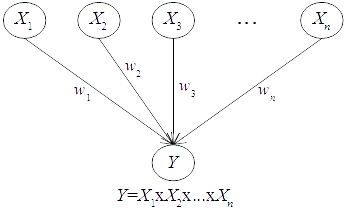
\includegraphics{SimpleGraph.png}
\caption{Simple graph or simple network}
\label{figure:simple-graph}
\end{figure}
%Figure 3.1. Simple graph or simple network

Child variable \textit{Y} is called target and parent variables \textit{X${}_{i}$} (s) are called sources. Especially, these relationships are adhere to X-gates such as AND-gate, OR-gate, and SIGMA-gate. These gates are originated from logic gate \cite{wikipedia:logic-gates}. For instance, AND-gate and OR-gate represent prerequisite relationship. SIGMA-gate represents aggregation relationship. Therefore, relationship conversion is to determined X-gate inference. The simple graph shown in figure~\ref{figure:simple-graph} is also called X-gate graph or X-gate network. Please distinguish the letter ``X'' in the term ``X-gate inference'' which implies logic operators (AND, OR, XOR, etc.) from the ``variable \textit{X}''.

All variables are binary and they represent events. The probability \textit{P}(\textit{X}) indicates event \textit{X} occurs. Thus, \textit{P}(\textit{X}) implicates \textit{P}(\textit{X}=1) and \textit{P}(not(\textit{X})) implicates \textit{P}(\textit{X}=0). Formula~\ref{formula:not-gate-inference} specifies the simple NOT-gate inference.

\begin{equation}
\begin{split} 
&P\left(\mathrm{not}\left(X\right)\right)=P\left(\overline{X}\right)=P\left(X=0\right)=1-P\left(X=1\right)=1-P\left(X\right)\\
&P\left(\mathrm{not}\left(\mathrm{not}\left(X\right)\right)\right)=P\left(X\right)
\end{split}
\label{formula:not-gate-inference}
\end{equation}
%Formula 3.1. NOT-gate inference

X-gate inference is based on three assumptions mentioned in \cite[p.~157]{neapolitan:bn}:

\begin{enumerate}
\item  \textit{X-gate inhibition}: Given a relationship from source \textit{X${}_{i}$} to target \textit{Y}, there is a factor \textit{I${}_{i}$} that inhibits \textit{X${}_{i}$} from integrated into \textit{Y}. Factor \textit{I${}_{i}$} is called inhibition of \textit{X${}_{i}$}. That the inhibition \textit{I${}_{i}$} is turned off is prerequisite of \textit{X${}_{i}$} integrated into \textit{Y}.

\item  \textit{Inhibition independence}: Inhibitions are mutually independent. For example, inhibition \textit{I}${}_{1}$ of \textit{X}${}_{1}$ is independent from inhibition \textit{I}${}_{2}$ of \textit{X}${}_{2}$.

\item  \textit{Accountability}: X-gate network is established by accountable variables \textit{A${}_{i}$} for \textit{X${}_{i}$} and \textit{I${}_{i}$}. Each X-gate inference owns particular combination of \textit{A${}_{i}$} (s).
\end{enumerate}

Figure~\ref{figure:extended-x-gate-network} shows the extended X-gate network with accountable variables \textit{A${}_{i}$} (s) \cite[p.~158]{neapolitan:bn}.

\begin{figure}
\centering
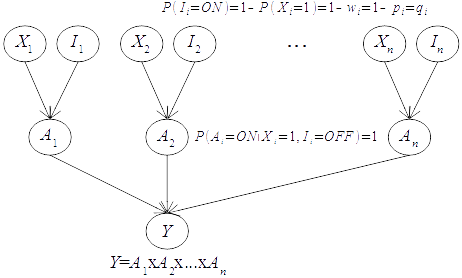
\includegraphics{ExtendedXgateNetwork.png}
\caption{Extended X-gate network with accountable variables \textit{A${}_{i}$} (s)}
\label{figure:extended-x-gate-network}
\end{figure}
%Figure 3.2. Extended X-gate network with accountable variables \textit{A${}_{i}$} (s)

The strength of each relationship from source \textit{X${}_{i}$} to target \textit{Y} is quantified by a weight 0 $\mathrm{\le}$ \textit{w${}_{i}$} $\mathrm{\le}$ 1. According to the assumption of inhibition, probability of \textit{I${}_{i}$}=\textit{OFF} is \textit{p${}_{i}$}, which is set to be the weight \textit{w${}_{i}$}.
\[p_i=w_i\] 
If notation \textit{w${}_{i}$} is used, we focus on strength of relationship. If notation \textit{p${}_{i}$} is used, we focus on probability of \textit{OFF} inhibition. In probabilistic inference, \textit{p${}_{i}$} is also prior probability of \textit{X${}_{i}$}=1. However, we will assume each \textit{X${}_{i}$} has uniform distribution later on. Formula~\ref{formula:inhibition-probs} specifies probabilities of inhibitions \textit{I${}_{i}$} (s) and accountable variables \textit{A${}_{i}$} (s).

\begin{equation}
\begin{split}
&P\left(I_i\mathrm{=}OFF\right)=p_i=w_i\\
&P\left(I_i\mathrm{=}ON\right)=1-p_i=1-w_i\\
&P\left(A_i\mathrm{=}ON\mathrel{\left|\vphantom{A_i\mathrm{=}ON X_i\mathrm{=1,}I_i\mathrm{=}OFF}\right.\kern-\nulldelimiterspace}X_i\mathrm{=1,}I_i\mathrm{=}OFF\right)\mathrm{=1}\\
&P\left(A_i\mathrm{=}ON\mathrel{\left|\vphantom{A_i\mathrm{=}ON X_i\mathrm{=1,}I_i\mathrm{=}ON}\right.\kern-\nulldelimiterspace}X_i\mathrm{=1,}I_i\mathrm{=}ON\right)\mathrm{=0}\\
&P\left(A_i\mathrm{=}ON\mathrel{\left|\vphantom{A_i\mathrm{=}ON X_i\mathrm{=0,}I_i\mathrm{=}OFF}\right.\kern-\nulldelimiterspace}X_i\mathrm{=0,}I_i\mathrm{=}OFF\right)\mathrm{=0}\\
&P\left(A_i\mathrm{=}ON\mathrel{\left|\vphantom{A_i\mathrm{=}ON X_i\mathrm{=0,}I_i\mathrm{=}ON}\right.\kern-\nulldelimiterspace}X_i\mathrm{=0,}I_i\mathrm{=}ON\right)\mathrm{=0}\\
&P\left(A_i\mathrm{=}OFF\mathrel{\left|\vphantom{A_i\mathrm{=}OFF X_i\mathrm{=1,}I_i\mathrm{=}OFF}\right.\kern-\nulldelimiterspace}X_i\mathrm{=1,}I_i\mathrm{=}OFF\right)\mathrm{=0}\\
&P\left(A_i\mathrm{=}OFF\mathrel{\left|\vphantom{A_i\mathrm{=}OFF X_i\mathrm{=1,}I_i\mathrm{=}ON}\right.\kern-\nulldelimiterspace}X_i\mathrm{=1,}I_i\mathrm{=}ON\right)\mathrm{=1}\\
&P\left(A_i\mathrm{=}OFF\mathrel{\left|\vphantom{A_i\mathrm{=}OFF X_i\mathrm{=0,}I_i\mathrm{=}OFF}\right.\kern-\nulldelimiterspace}X_i\mathrm{=0,}I_i\mathrm{=}OFF\right)\mathrm{=1}\\
&P\left(A_i\mathrm{=}OFF\mathrel{\left|\vphantom{A_i\mathrm{=}OFF X_i\mathrm{=0,}I_i\mathrm{=}ON}\right.\kern-\nulldelimiterspace}X_i\mathrm{=0,}I_i\mathrm{=}ON\right)\mathrm{=1}
\end{split}
\label{formula:inhibition-probs}
\end{equation} 
%Formula 3.2. Probabilities of inhibitions \textit{I${}_{i}$} (s) and accountable variables \textit{A${}_{i}$} (s)

According to formula~\ref{formula:inhibition-probs}, given probability \textit{P}(\textit{A${}_{i}$}=\textit{ON} {\textbar} \textit{X${}_{i}$}=1, \textit{I${}_{i}$}=\textit{OFF}), it is assured 100\% confident that accountable variables \textit{A${}_{i}$} is turned on if source \textit{X${}_{i}$} is 1 and inhibition \textit{I${}_{i}$} is turned off. Formula~\ref{formula:accountable-probs} specifies conditional probability of accountable variables \textit{A${}_{i}$} (s) given \textit{X${}_{i}$} (s), which is corollary of formula~\ref{formula:inhibition-probs}.

\begin{equation}
\begin{split} 
&P\left(A_i=ON\mathrel{\left|\vphantom{A_i=ON X_i=1}\right.\kern-\nulldelimiterspace}X_i=1\right)=p_i=w_i\\
&P\left(A_i=ON\mathrel{\left|\vphantom{A_i=ON X_i=0}\right.\kern-\nulldelimiterspace}X_i=0\right)=0\\
&P\left(A_i=OFF\mathrel{\left|\vphantom{A_i=OFF X_i=1}\right.\kern-\nulldelimiterspace}X_i=1\right)=1-p_i=1-w_i\\
&P\left(A_i=OFF\mathrel{\left|\vphantom{A_i=OFF X_i=0}\right.\kern-\nulldelimiterspace}X_i=0\right)=1
\end{split}
\label{formula:accountable-probs}
\end{equation}
%Formula 3.3. Conditional probability of accountable variables

Following is proof of formula~\ref{formula:accountable-probs}.
\begin{align*}
&P\left(A_i=ON\mathrel{\left|\vphantom{A_i=ON X_i}\right.\kern-\nulldelimiterspace}X_i\right)=P\left(A_i=ON\mathrel{\left|\vphantom{A_i=ON X_i,I_i=ON}\right.\kern-\nulldelimiterspace}X_i,I_i=ON\right)P\left(I_i=ON\right)\\
&+P\left(A_i=ON\mathrel{\left|\vphantom{A_i=ON X_i,I_i=OFF}\right.\kern-\nulldelimiterspace}X_i,I_i=OFF\right)P\left(I_i=OFF\right)\\
&=0*\left(1-p_i\right)+P\left(A_i=ON\mathrel{\left|\vphantom{A_i=ON X_i,I_i=OFF}\right.\kern-\nulldelimiterspace}X_i,I_i=OFF\right)p_i\\
&\left(\mathrm{By\ applying\ formula\ \ref{formula:inhibition-probs}}\right)\\
&=p_iP\left(A_i=ON\mathrel{\left|\vphantom{A_i=ON X_i,I_i=OFF}\right.\kern-\nulldelimiterspace}X_i,I_i=OFF\right)
\end{align*}
It implies
\begin{align*}
&P\left(A_i=ON\mathrel{\left|\vphantom{A_i=ON X_i=1}\right.\kern-\nulldelimiterspace}X_i=1\right)=p_iP\left(A_i=ON\mathrel{\left|\vphantom{A_i=ON X_i=1,I_i=OFF}\right.\kern-\nulldelimiterspace}X_i=1,I_i=OFF\right)=p_i\\
&P\left(A_i=ON\mathrel{\left|\vphantom{A_i=ON X_i=0}\right.\kern-\nulldelimiterspace}X_i=0\right)=p_iP\left(A_i=ON\mathrel{\left|\vphantom{A_i=ON X_i=0,I_i=OFF}\right.\kern-\nulldelimiterspace}X_i=0,I_i=OFF\right)=0\\
&P\left(A_i=OFF\mathrel{\left|\vphantom{A_i=OFF X_i=1}\right.\kern-\nulldelimiterspace}X_i=1\right)=1-P\left(A_i=ON\mathrel{\left|\vphantom{A_i=ON X_i=1}\right.\kern-\nulldelimiterspace}X_i=1\right)=1-p_i\\
&P\left(A_i=OFF\mathrel{\left|\vphantom{A_i=OFF X_i=0}\right.\kern-\nulldelimiterspace}X_i=0\right)=1-P\left(A_i=ON\mathrel{\left|\vphantom{A_i=ON X_i=0}\right.\kern-\nulldelimiterspace}X_i=0\right)=1
\end{align*}
As a definition, the set of all \textit{X${}_{i}$} (s) is complete if and only if
\[P\left(X_1\cup X_2\cup \cdots \cup X_n\right)=P\left(\mathrm{\Omega }\right)=\sum^n_{i=1}{w_i}=1\] 
The set of all \textit{X${}_{i}$} (s) is mutually exclusive if and only if
\[X_i\cap X_j=\emptyset ,\forall i\neq j\] 
For each \textit{X${}_{i}$} there is only one \textit{A${}_{i}$} and vice versa, which establishes a bijection between \textit{X${}_{i}$} (s) and \textit{A${}_{i}$} (s). Obviously, the fact that the set of all \textit{X${}_{i}$} (s) is complete is equivalent to the fact that the set of all \textit{A${}_{i}$} (s) is complete. We will prove by contradiction that ``the fact that the set of all \textit{X${}_{i}$} (s) is mutually exclusive is equivalent to the fact that the set of all \textit{A${}_{i}$} (s) is mutually exclusive''. Suppose $X_i\cap X_j=\emptyset ,\forall i\neq j$ but $\exists i\neq j$: $A_i\cap A_j=B\neq \emptyset $. Let $B^{-1}\neq \emptyset $ be preimage of \textit{B}. Due to $B\subseteq A_i$ and $B\subseteq A_j$, we have $B^{-1}\subseteq X_i$ and $B^{-1}\subseteq X_j$, which causes that $X_i\cap X_j=B^{-1}\neq \emptyset $. There is a contradiction and so we have:
\[X_i\cap X_j=\emptyset ,\forall i\neq j\Rightarrow A_i\cap A_j=\emptyset ,\forall i\neq j\] 
By similar proof, we have:
\[A_i\cap A_j=\emptyset ,\forall i\neq j\Rightarrow X_i\cap X_j=\emptyset ,\forall i\neq j\] 
The extended X-gate network shown in figure~\ref{figure:extended-x-gate-network} is interpretation of simple network shown in figure~\ref{figure:simple-graph}. Specifying CPT of the simple network is to determine the conditional probability \textit{P}(\textit{Y}=1 {\textbar} \textit{X}${}_{1}$, \textit{X}${}_{2}$,{\dots}, \textit{X${}_{n}$}) based on extended X-gate network. The X-gate inference is represented by such probability \textit{P}(\textit{Y}=1 {\textbar} \textit{X}${}_{1}$, \textit{X}${}_{2}$,{\dots}, \textit{X${}_{n}$}) specified by formula~\ref{formula:x-gate-prob} \cite[p.~159]{neapolitan:bn}.

\begin{equation}
P\left(Y\mathrel{\left|\vphantom{Y X_1,X_2,\dots ,X_n}\right.\kern-\nulldelimiterspace}X_1,X_2,\dots ,X_n\right)=\sum_{A_1,A_2,\dots ,A_n}{P\left(Y\mathrel{\left|\vphantom{Y A_1,A_2,\dots ,A_n}\right.\kern-\nulldelimiterspace}A_1,A_2,\dots ,A_n\right)\prod^n_{i=1}{P\left(A_i\mathrel{\left|\vphantom{A_i X_i}\right.\kern-\nulldelimiterspace}X_i\right)}}
\label{formula:x-gate-prob}
\end{equation}
%Formula 3.4. X-gate probability

Following is the proof of formula~\ref{formula:x-gate-prob}.
\begin{align*}
&P\left(Y\mathrel{\left|\vphantom{Y X_1,X_2,\dots ,X_n}\right.\kern-\nulldelimiterspace}X_1,X_2,\dots ,X_n\right)=\frac{P\left(Y,X_1,X_2,\dots ,X_n\right)}{P\left(X_1,X_2,\dots ,X_n\right)}\\
&\left(\mathrm{Due\ to\ Bayes'\ rule}\right)\\
&=\frac{\sum_{A_1,A_2,\dots ,A_n}{P\left(Y,X_1,X_2,\dots ,X_n\mathrel{\left|\vphantom{Y,X_1,X_2,\dots ,X_n A_1,A_2,\dots ,A_n}\right.\kern-\nulldelimiterspace}A_1,A_2,\dots ,A_n\right)*P\left(A_1,A_2,\dots ,A_n\right)}}{P\left(X_1,X_2,\dots ,X_n\right)}\\
&\left(\mathrm{Due\ to\ total\ probability\ rule}\right)\\
&=\sum_{A_1,A_2,\dots ,A_n}{P\left(Y,X_1,X_2,\dots ,X_n\mathrel{\left|\vphantom{Y,X_1,X_2,\dots ,X_n A_1,A_2,\dots ,A_n}\right.\kern-\nulldelimiterspace}A_1,A_2,\dots ,A_n\right)*\frac{P\left(A_1,A_2,\dots ,A_n\right)}{P\left(X_1,X_2,\dots ,X_n\right)}}\\
&\begin{aligned}
=\sum_{A_1,A_2,\dots ,A_n}{P\left(Y\mathrel{\left|\vphantom{Y A_1,A_2,\dots ,A_n}\right.\kern-\nulldelimiterspace}A_1,A_2,\dots ,A_n\right)*P\left(X_1,X_2,\dots ,X_n\mathrel{\left|\vphantom{X_1,X_2,\dots ,X_n A_1,A_2,\dots ,A_n}\right.\kern-\nulldelimiterspace}A_1,A_2,\dots ,A_n\right)}\\
*\frac{P\left(A_1,A_2,\dots ,A_n\right)}{P\left(X_1,X_2,\dots ,X_n\right)}
\end{aligned}\\
&\left(\mathrm{Because}\ Y\ \mathrm{is\ conditionally\ independent\ from}\ X_i\ \mathrm{(s)}\ \mathrm{given}\ A_i\ \mathrm{(s)}\right)\\
&=\sum_{A_1,A_2,\dots ,A_n}{P\left(Y\mathrel{\left|\vphantom{Y A_1,A_2,\dots ,A_n}\right.\kern-\nulldelimiterspace}A_1,A_2,\dots ,A_n\right)*\frac{P\left(X_1,X_2,\dots ,X_n,A_1,A_2,\dots ,A_n\right)}{P\left(X_1,X_2,\dots ,X_n\right)}}\\
&=\sum_{A_1,A_2,\dots ,A_n}{P\left(Y\mathrel{\left|\vphantom{Y A_1,A_2,\dots ,A_n}\right.\kern-\nulldelimiterspace}A_1,A_2,\dots ,A_n\right)*P\left(A_1,A_2,\dots ,A_n\mathrel{\left|\vphantom{A_1,A_2,\dots ,A_n X_1,X_2,\dots ,X_n}\right.\kern-\nulldelimiterspace}X_1,X_2,\dots ,X_n\right)}\\
&\left(\mathrm{Due\ to\ Bayes'\ rule}\right)\\
&=\sum_{A_1,A_2,\dots ,A_n}{P\left(Y\mathrel{\left|\vphantom{Y A_1,A_2,\dots ,A_n}\right.\kern-\nulldelimiterspace}A_1,A_2,\dots ,A_n\right)\prod^n_{i=1}{P\left(A_i\mathrel{\left|\vphantom{A_i X_1,X_2,\dots ,X_n}\right.\kern-\nulldelimiterspace}X_1,X_2,\dots ,X_n\right)}}\\
&\left(\mathrm{Because}\ A_i\ \mathrm{(s)}\ \mathrm{are\ mutually\ independent}\right)\\
&=\sum_{A_1,A_2,\dots ,A_n}{P\left(Y\mathrel{\left|\vphantom{Y A_1,A_2,\dots ,A_n}\right.\kern-\nulldelimiterspace}A_1,A_2,\dots ,A_n\right)\prod^n_{i=1}{P\left(A_i\mathrel{\left|\vphantom{A_i X_i}\right.\kern-\nulldelimiterspace}X_i\right)}}\\
&\left(\mathrm{Because}\ \mathrm{each}\ A_i\ \mathrm{is\ only\ dependent\ on}\ X_i\right)
\end{align*}

It is necessary to make some mathematical notations because formula~\ref{formula:x-gate-prob} is complicated, which is relevant to arrangements of \textit{X${}_{i}$} (s). Given $\Omega$ = $\{$\textit{X}${}_{1}$, \textit{X}${}_{2}$,{\dots}, \textit{X${}_{n}$}$\}$ is set of binary variables and $|\Omega|$=\textit{n} is cardinality of $\Omega$.

Let \textit{a}($\Omega$) be an arrangement of $\Omega$ which is a set of \textit{n} instances $\{$\textit{X}${}_{1}$=\textit{x}${}_{1}$, \textit{X}${}_{2}$=\textit{x}${}_{2}$,{\dots}, \textit{X${}_{n}$}=\textit{x${}_{n}$}$\}$ where \textit{x${}_{i}$} is 1 or 0. The number of all \textit{a}($\Omega$) is $2^{|\Omega|}$. For instance, given $\Omega$ = $\{$\textit{X}${}_{1}$, \textit{X}${}_{2}$$\}$, there are 2${}^{2}$=4 arrangements as follows:
\begin{align*}
&a\left\{\Omega\right\}=\left\{X_1=1,X_2=1\right\}\\
&a\left\{\Omega\right\}=\left\{X_1=1,X_2=0\right\}\\
&a\left\{\Omega\right\}=\left\{X_1=0,X_2=1\right\}\\
&a\left\{\Omega\right\}=\left\{X_1=0,X_2=0\right\}
\end{align*}
Let \textit{a}($\Omega$:$\{$\textit{X${}_{i}$}$\}$) be the arrangement of $\Omega$ with fixed \textit{X${}_{i}$}. The number of all \textit{a}($\Omega$:$\{$\textit{X${}_{i}$}$\}$) is $2^{|\Omega|-1}$. Similarly, for instance, \textit{a}($\Omega$:$\{$\textit{X}${}_{1}$, \textit{X}${}_{2}$, \textit{X}${}_{3}$$\}$) is an arrangement of $\Omega$ with fixed \textit{X}${}_{1}$, \textit{X}${}_{2}$, \textit{X}${}_{3}$. The number of all \textit{a}($\Omega$:$\{$\textit{X}${}_{1}$, \textit{X}${}_{2}$, \textit{X}${}_{3}$$\}$) is $2^{|\Omega|-3}$.

Let \textit{c}($\Omega$) and \textit{c}($\Omega$:$\{$\textit{X${}_{i}$}$\}$) be the number of arrangements \textit{a}($\Omega$) and \textit{a}($\Omega$:$\{$\textit{X${}_{i}$}$\}$), respectively. Such \textit{c}($\Omega$) and \textit{c}($\Omega$:$\{$\textit{X${}_{i}$}$\}$) are called arrangement counters. As usual, counters \textit{c}($\Omega$) and \textit{c}($\Omega$:$\{$\textit{X${}_{i}$}$\}$) are equal to $2^{|\Omega|}$ and $2^{|\Omega|-1}$, respectively but they will vary according to specific cases.

Let $\sum_a{F\left(a\left(\mathrm{\Omega }\right)\right)}$ and $\prod_a{F\left(a\left(\mathrm{\Omega }\right)\right)}$ denote sum and product of values generated from function \textit{F} acting on every \textit{a}($\Omega$). The number of arrangements on which \textit{F} acts is \textit{c}($\Omega$).

Let x denote the X-gate operator, for instance, $\mathrm{x}=\odot $ for AND-gate, $\mathrm{x}=\oplus $ for OR-gate, $\mathrm{x}=\mathrm{not}\odot $ for NAND-gate, $\mathrm{x}=\mathrm{not}\oplus $ for NOR-gate, $\mathrm{x}=\otimes $ for XOR-gate, $\mathrm{x}=\mathrm{not}\otimes $ for XNOR-gate, $\mathrm{x}=\uplus $ for U-gate, $\mathrm{x}=+$ for SIGMA-gate. Given an x-operator, let \textit{s}($\Omega$:$\{$\textit{X${}_{i}$}$\}$) and \textit{s}($\Omega$) be sum of all $P\left(X_1\mathrm{x}X_2\mathrm{x}\dots \mathrm{x}X_n\right)$ through every arrangement of $\Omega$ with and without fixed \textit{X${}_{i}$}, respectively. Such \textit{s}($\Omega$) and \textit{s}($\Omega$:$\{$\textit{X${}_{i}$}$\}$) are called arrangement sum according to definition~\ref{definition:binary-arrangements}. They are acting function \textit{F}.

\begin{definition}
$\begin{aligned}
s\left(\mathrm{\Omega }\right)&=\sum_a{P\left(X_1\mathrm{x}X_2\mathrm{x}\dots \mathrm{x}X_n\mathrel{\left|\vphantom{X_1\mathrm{x}X_2\mathrm{x}\dots \mathrm{x}X_n a\left(\mathrm{\Omega }\right)}\right.\kern-\nulldelimiterspace}a\left(\mathrm{\Omega }\right)\right)}\\
&=\sum_a{P\left(Y=1\mathrel{\left|\vphantom{Y=1 a\left(\mathrm{\Omega }\right)}\right.\kern-\nulldelimiterspace}a\left(\mathrm{\Omega }\right)\right)}\\
s\left(\mathrm{\Omega }\mathrm{:}\left\{X_i\right\}\right)&=\sum_a{P\left(X_1\mathrm{x}X_2\mathrm{x}\dots \mathrm{x}X_n\mathrel{\left|\vphantom{X_1\mathrm{x}X_2\mathrm{x}\dots \mathrm{x}X_n a\left(\mathrm{\Omega }\mathrm{:}\left\{X_i\right\}\right)}\right.\kern-\nulldelimiterspace}a\left(\mathrm{\Omega }\mathrm{:}\left\{X_i\right\}\right)\right)}\\
&=\sum_a{P\left(Y=1\mathrel{\left|\vphantom{Y=1 a\left(\mathrm{\Omega }\mathrm{:}\left\{X_i\right\}\right)}\right.\kern-\nulldelimiterspace}a\left(\mathrm{\Omega }\mathrm{:}\left\{X_i\right\}\right)\right)}
\end{aligned}$
\label{definition:binary-arrangements}
\end{definition}
%Table 3.1. Binary arrangements
For example, \textit{s}($\Omega$) and \textit{s}($\Omega$:$\{$\textit{X${}_{i}$}$\}$) for OR-gate are:
\begin{align*}
s\left(\mathrm{\Omega }\right)&=\sum_a{P\left(X_1\oplus X_2\oplus \dots \oplus X_n\mathrel{\left|\vphantom{X_1\oplus X_2\oplus \dots \oplus X_n a\left(\mathrm{\Omega }\right)}\right.\kern-\nulldelimiterspace}a\left(\mathrm{\Omega }\right)\right)}\\
s\left(\mathrm{\Omega }\mathrm{:}\left\{X_i\right\}\right)&=\sum_a{P\left(X_1\oplus X_2\oplus \dots \oplus X_n\mathrel{\left|\vphantom{X_1\oplus X_2\oplus \dots \oplus X_n a\left(\mathrm{\Omega }\mathrm{:}\left\{X_i\right\}\right)}\right.\kern-\nulldelimiterspace}a\left(\mathrm{\Omega }\mathrm{:}\left\{X_i\right\}\right)\right)}
\end{align*}
Note that $\Omega$ can be any set of binary variables.

It is not easy to produce all binary arrangements of $\Omega$. The following is code snippet written by Java programming language for producing such all arrangements.

\begin{lstlisting}[language = Java]
public class Generator {
  private ArrayList<int[]> arrangements;
  private int n;
  private int r;

  private Generator(int n, int r) {
    this.n = n;
    this.r = r;
    this.arrangements = new ArrayList();
  }

  private void create(int[] a, int i) {
    for(int j = 0; j < n; j++) {
      a[i] = j;
      if(i < r - 1)
        create(a, i + 1);
      else if(i == r -1) {
        int[] b = new int[a.length];
        for(int k = 0; k < a.length; k++)
          b[k] = a[k];
        arrangements.add(b);
      }
    }
  }

  public int[] get(int i) {
    return arrangements.get(i);
  }

  public long size() {
    return arrangements.size();
  }

  public static Generator parse(int n, int r) {
    Generator arr =
      new Generator(n, r);
    int[] a = new int[r];
    for(int i=0; i<r; i++) a[i] = -1;
    arr.create(a, 0);
    return arr;
  }
}
\end{lstlisting}
%Table 3.2. Code snippet generating all binary arrangements

Each element of the list ``\textit{arrangements}'' is a binary arrangement \textit{a}($\Omega$) presented by an array of bits (0 and 1). The method ``\textit{create}(\textit{int}[] \textit{a}, \textit{int i})'' which is recursive method, is the main one that generates arrangements. The method call ``\textit{Generator}.\textit{parse}(2, \textit{n})'' will list all possible binary arrangements.

Formula~\ref{formula:arrangement-sum-counter} specifies the connection between \textit{s}($\Omega$:$\{$\textit{X${}_{i}$}=1$\}$) and \textit{s}($\Omega$:$\{$\textit{X${}_{i}$}=0$\}$), between \textit{c}($\Omega$:$\{$\textit{X${}_{i}$}=1$\}$) and \textit{c}($\Omega$:$\{$\textit{X${}_{i}$}=0$\}$).

\begin{equation}
\begin{split}
&s\left(\mathrm{\Omega }\mathrm{:}\left\{X_i=1\right\}\right)+s\left(\mathrm{\Omega }\mathrm{:}\left\{X_i=0\right\}\right)=s\left(\mathrm{\Omega }\right)\\
&c\left(\mathrm{\Omega }\mathrm{:}\left\{X_i=1\right\}\right)+c\left(\mathrm{\Omega }\mathrm{:}\left\{X_i=0\right\}\right)=c\left(\mathrm{\Omega }\right)
\end{split}
\label{formula:arrangement-sum-counter}
\end{equation} 
%Formula 3.5. Connection among arrangement sum and counter

It is easy to draw formula~\ref{formula:arrangement-sum-counter} when the set of all arrangements \textit{a}($\Omega$:$\{$\textit{X${}_{i}$}=1) is complement of the set of all arrangements \textit{a}($\Omega$:$\{$\textit{X${}_{i}$}=0).

Let \textit{K} be a set of \textit{X${}_{i}$} (s) whose values are 1 and let \textit{L} be a set of \textit{X${}_{i}$} (s) whose values are 0. \textit{K} and \textit{L} are mutually complementary. Formula~\ref{formula:sets-k-l} determines sets \textit{K} and \textit{L}.

\begin{equation}
\left\{ \begin{array}{l}
K=\left\{i:X_i=1\right\} \\ 
L=\left\{i:X_i=0\right\} \\ 
K\cap L=\emptyset  \\ 
K\cup L=\{1,2,\dots ,n\} \end{array}
\right.
\label{formula:sets-k-l}
\end{equation}
%Formula 3.6. Sets \textit{K} and \textit{L}

The \textbf{AND-gate} inference represents prerequisite relationship satisfying AND-gate condition specified by formula~\ref{formula:and-gate-condition}.

\begin{equation} 
P\left(Y\mathrm{=1}\mathrel{\left|\vphantom{Y\mathrm{=1} A_i\mathrm{=}OFF\mathrm{\ for\ some\ }i}\right.\kern-\nulldelimiterspace}A_i\mathrm{=}OFF\mathrm{\ for\ some\ }i\right)\mathrm{=0}
\label{formula:and-gate-condition}
\end{equation}
%Formula 3.7. AND-gate condition

From formula~\ref{formula:x-gate-prob}, we have
\begin{align*}
&P\left(Y=1\mathrel{\left|\vphantom{Y=1 X_1,X_2,\dots ,X_n}\right.\kern-\nulldelimiterspace}X_1,X_2,\dots ,X_n\right)\\
&=\sum_{A_1,A_2,\dots ,A_n}{P\left(Y=1\mathrel{\left|\vphantom{Y=1 A_1,A_2,\dots ,A_n}\right.\kern-\nulldelimiterspace}A_1,A_2,\dots ,A_n\right)\prod^n_{i=1}{P\left(A_i\mathrel{\left|\vphantom{A_i X_i}\right.\kern-\nulldelimiterspace}X_i\right)}}\\ 
&=\prod^n_{i=1}{P\left(A_i=ON\mathrel{\left|\vphantom{A_i=ON X_i}\right.\kern-\nulldelimiterspace}X_i\right)}\\ 
&\left(\mathrm{due\ to\ }P\left(Y=1\mathrel{\left|\vphantom{Y=1 A_i=OFF\ \mathrm{for\ some}\ i}\right.\kern-\nulldelimiterspace}A_i=OFF\ \mathrm{for\ some}\ i\right)=0\right)\\
&=\left(\prod_{i\in K}{P\left(A_i=ON\mathrel{\left|\vphantom{A_i=ON X_i=1}\right.\kern-\nulldelimiterspace}X_i=1\right)}\right)\left(\prod_{i\notin K}{P\left(A_i=ON\mathrel{\left|\vphantom{A_i=ON X_i=0}\right.\kern-\nulldelimiterspace}X_i=0\right)}\right)\\
&=\left(\prod_{i\in K}{p_i}\right)\left(\prod_{i\notin K}{0}\right)\\
&=\left\{ \begin{array}{l}
\prod^n_{i=1}{p_i}\ \mathrm{if\ all}\ X_i\ \left(s\right)\ \mathrm{are}\ 1 \\ 
0\ \mathrm{if\ there\ exists\ at\ least\ one\ }X_i=0 \end{array}
\right.\\
&\left(\mathrm{Due}\ \mathrm{to}\ \mathrm{formula}\ \mathrm{\ref{formula:accountable-probs}}\right)
\end{align*}

In general, formula~\ref{formula:and-gate-inference} specifies AND-gate inference.

\begin{equation}
\begin{split}
P\left(X_1\odot X_2\odot \dots \odot X_n\right)&=P\left(Y=1\mathrel{\left|\vphantom{Y=1 X_1,X_2,\dots ,X_n}\right.\kern-\nulldelimiterspace}X_1,X_2,\dots ,X_n\right)\\
&=\left\{ \begin{array}{l}
\prod^n_{i=1}{p_i}\ \mathrm{if\ all}\ X_i\ \left(s\right)\ \mathrm{are}\ 1 \\ 
0\ \mathrm{if\ there\ exists\ at\ least\ one\ }X_i=0 \end{array}
\right.\\
P\left(Y=0\mathrel{\left|\vphantom{Y=0 X_1,X_2,\dots ,X_n}\right.\kern-\nulldelimiterspace}X_1,X_2,\dots ,X_n\right)&=\left\{ \begin{array}{l}
1-\prod^n_{i=1}{p_i}\ \mathrm{if\ all}\ X_i\ \left(s\right)\ \mathrm{are}\ 1 \\ 
1\ \mathrm{if\ there\ exists\ at\ least\ one\ }X_i=0 \end{array}
\right.
\end{split}
\label{formula:and-gate-inference}
\end{equation}
%Formula 3.8. AND-gate inference

The AND-gate formula was also described in \cite[p.~33]{diez:pmodels}. Formula~\ref{formula:and-gate-inference} varies according to two cases whose arrangement counters are listed as follows:
\begin{center}
\begin{tabular}{l|l}
$L=\emptyset$ &
  $\begin{aligned}
  c\left(\mathrm{\Omega }:\left\{X_i=1\right\}\right)&=1\\
  c\left(\mathrm{\Omega }:\left\{X_i=0\right\}\right)&=0\\
  c\left(\mathrm{\Omega }\right)&=1
  \end{aligned}$\\
\hline
$L\neq \emptyset$ &
  $\begin{aligned}
  c\left(\mathrm{\Omega }:\left\{X_i=1\right\}\right)&=2^{n-1}-1\\
  c\left(\mathrm{\Omega }:\left\{X_i=0\right\}\right)&=2^{n-1}\\
  c\left(\mathrm{\Omega }\right)&=2^n-1
  \end{aligned}$\\
\end{tabular}
\end{center}
The \textbf{OR-gate} inference represents prerequisite relationship satisfying OR-gate condition specified by formula~\ref{formula:or-gate-condition} \cite[p.~157]{neapolitan:bn}.

\begin{equation}
P\left(Y\mathrm{=1}\mathrel{\left|\vphantom{Y\mathrm{=1} A_i\mathrm{=}ON\mathrm{\ for\ some\ }i}\right.\kern-\nulldelimiterspace}A_i\mathrm{=}ON\mathrm{\ for\ some\ }i\right)\mathrm{=1}
\label{formula:or-gate-condition}
\end{equation}
%Formula 3.9. OR-gate condition

The OR-gate condition implies
\[P\left(Y\mathrm{=0}\mathrel{\left|\vphantom{Y\mathrm{=0} A_i\mathrm{=}ON\mathrm{\ for\ some\ }i}\right.\kern-\nulldelimiterspace}A_i\mathrm{=}ON\mathrm{\ for\ some\ }i\right)\mathrm{=0}\] 
From formula~\ref{formula:x-gate-prob}, we have \cite[p.~159]{neapolitan:bn}:
\begin{align*}
&P\left(Y=0\mathrel{\left|\vphantom{Y=0 X_1,X_2,\dots ,X_n}\right.\kern-\nulldelimiterspace}X_1,X_2,\dots ,X_n\right)\\
&=\sum_{A_1,A_2,\dots ,A_n}{P\left(Y=1\mathrel{\left|\vphantom{Y=1 A_1,A_2,\dots ,A_n}\right.\kern-\nulldelimiterspace}A_1,A_2,\dots ,A_n\right)\prod^n_{i=1}{P\left(A_i\mathrel{\left|\vphantom{A_i X_i}\right.\kern-\nulldelimiterspace}X_i\right)}}\\ 
&=\prod^n_{i=1}{P\left(A_i=OFF\mathrel{\left|\vphantom{A_i=OFF X_i}\right.\kern-\nulldelimiterspace}X_i\right)}\\
&\left(\mathrm{due\ to\ }P\left(Y=1\mathrel{\left|\vphantom{Y=1 A_i=ON\ \mathrm{for\ some}\ i}\right.\kern-\nulldelimiterspace}A_i=ON\ \mathrm{for\ some}\ i\right)=0\right)\\
&=\left(\prod_{i\in K}{P\left(A_i=OFF\mathrel{\left|\vphantom{A_i=OFF X_i=1}\right.\kern-\nulldelimiterspace}X_i=1\right)}\right)\left(\prod_{i\notin K}{P\left(A_i=OFF\mathrel{\left|\vphantom{A_i=OFF X_i=0}\right.\kern-\nulldelimiterspace}X_i=0\right)}\right)\\
&=\left(\prod_{i\in K}{\left(1-p_i\right)}\right)\left(\prod_{i\notin K}{1}\right)\\
&=\left\{ \begin{array}{r}
\prod_{i\in K}{\left(1-p_i\right)}\ \mathrm{if}\ K\neq \emptyset  \\ 
1\ \ \mathrm{if}\ K=\emptyset  \end{array}
\right.\\
&\left(\mathrm{Due}\ \mathrm{to}\ \mathrm{formula}\ \mathrm{\ref{formula:accountable-probs}}\right)
\end{align*}

In general, formula~\ref{formula:or-gate-inference} specifies OR-gate inference.

\begin{equation}
\begin{split}
P\left(X_1\oplus X_2\oplus \dots \oplus X_n\right)&=1-P\left(Y=0\mathrel{\left|\vphantom{Y=0 X_1,X_2,\dots ,X_n}\right.\kern-\nulldelimiterspace}X_1,X_2,\dots ,X_n\right)\\
&=\left\{ \begin{array}{r}
1-\prod_{i\in K}{\left(1-p_i\right)}\ \mathrm{if}\ K\neq \emptyset  \\ 
0\ \ \mathrm{if}\ K=\emptyset  \end{array}
\right.\\
P\left(Y=0\mathrel{\left|\vphantom{Y=0 X_1,X_2,\dots ,X_n}\right.\kern-\nulldelimiterspace}X_1,X_2,\dots ,X_n\right)&=\left\{ \begin{array}{r}
\prod_{i\in K}{\left(1-p_i\right)}\ \mathrm{if}\ K\neq \emptyset  \\ 
1\ \ \mathrm{if}\ K=\emptyset  \end{array}
\right.
\end{split}
\label{formula:or-gate-inference}
\end{equation}
%Formula 3.10. OR-gate inference

Where $K$ is the set of $X_i$ (s) whose values are 1. The OR-gate formula was mentioned in \cite[p.~158]{neapolitan:bn} and \cite[p.~20]{diez:pmodels}. Formula~\ref{formula:or-gate-inference} varies according to two cases whose arrangement counters are listed as follows:
\begin{center}
\begin{tabular}{l|l}
$K\neq \emptyset$ &
  $\begin{aligned}
  c\left(\mathrm{\Omega }:\left\{X_i=1\right\}\right)&=2^{n-1}\\
  c\left(\mathrm{\Omega }:\left\{X_i=0\right\}\right)&=2^{n-1}-1\\
  c\left(\mathrm{\Omega }\right)&=2^n-1
  \end{aligned}$\\
\hline
$K=\emptyset$ &
  $\begin{aligned}
  c\left(\mathrm{\Omega }:\left\{X_i=1\right\}\right)&=0\\
  c\left(\mathrm{\Omega }:\left\{X_i=0\right\}\right)&=1\\
  c\left(\mathrm{\Omega }\right)&=1
  \end{aligned}$
\end{tabular}
\end{center}
According to De Morgan's rule with regard to AND-gate and OR-gate, we have:
\begin{align*}
P\left(\mathrm{not}\left(X_1\odot X_2\odot \dots \odot X_n\right)\right)&=P\left(\left(\mathrm{not}\left(X_1\right)\right)\oplus \left(\mathrm{not}\left(X_2\right)\right)\oplus \dots \oplus \left(\mathrm{not}\left(X_n\right)\right)\right)\\
&=\left\{ \begin{array}{r}
1-\prod_{i\in L}{\left(1-\left(1-p_i\right)\right)}\ \mathrm{if}\ L\neq \emptyset  \\ 
0\ \ \mathrm{if}\ L=\emptyset  \end{array}
\right.\\
&\left(\mathrm{Due\ to\ formula~\ref{formula:or-gate-inference}}\right)
\end{align*}

According to formula~\ref{formula:and-gate-inference}, we also have:
\begin{align*}
P\left(\mathrm{not}\left(X_1\oplus X_2\oplus \dots \oplus X_n\right)\right)&=P\left(\left(\mathrm{not}\left(X_1\right)\right)\odot \left(\mathrm{not}\left(X_2\right)\right)\odot \dots \odot \left(\mathrm{not}\left(X_n\right)\right)\right)\\
&=\left\{ \begin{array}{l}
\prod^n_{i=1}{P\left(\mathrm{not}\left(X_i\right)\right)}\ \mathrm{if\ all}\ \mathrm{not}\left(X_i\right)\ \left(s\right)\ \mathrm{are}\ 1 \\ 
0\ \mathrm{if\ there\ exists\ at\ least\ one\ not}\left(X_i\right)=0 \end{array}
\right.\\
&=\left\{ \begin{array}{l}
\prod^n_{i=1}{\left(1-p_i\right)}\ \mathrm{if\ all}\ X_i\ \left(s\right)\ \mathrm{are}\ 0 \\ 
0\ \mathrm{if\ there\ exists\ at\ least\ one\ }X_i=1 \end{array}
\right.
\end{align*}
In general, formula~\ref{formula:nand-nor-gates-inference} specifies NAND-gate inference and NOR-gate inference derived from AND-gate and OR-gate:

\begin{equation}
\begin{split}
&P\left(\mathrm{not}\left(X_1\odot X_2\odot \dots \odot X_n\right)\right)=\left\{ \begin{array}{r}
1-\prod_{i\in L}{p_i}\ \mathrm{if}\ L\neq \emptyset  \\ 
0\ \ \mathrm{if}\ L=\emptyset  \end{array}
\right.\\
&P\left(\mathrm{not}\left(X_1\oplus X_2\oplus \dots \oplus X_n\right)\right)=\left\{ \begin{array}{r}
\prod^n_{i=1}{q_i}\ \mathrm{if\ }K=\emptyset  \\ 
0\ \mathrm{if\ }K\neq \emptyset  \end{array}
\right.
\end{split}
\label{formula:nand-nor-gates-inference}
\end{equation}
%Formula 3.11. NAND-gate inference and NOR-gate inference
Where $K$ and $L$ are the sets of $X_i$ (s) whose values are 1 and 0, respectively.

Suppose the number of sources \textit{X${}_{i}$} (s) is even. Let \textit{O} be the set of \textit{X${}_{i}$} (s) whose indices are odd. Let \textit{O}${}_{1}$ and \textit{O}${}_{2}$ be subsets of \textit{O}, in which all \textit{X${}_{i}$} (s) are 1 and 0, respectively. Let \textit{E} be the set of \textit{X${}_{i}$} (s) whose indices are even. Let \textit{E}${}_{1}$ and \textit{E}${}_{2}$ be subsets of \textit{E}, in which all \textit{X${}_{i}$} (s) are 1 and 0, respectively.
\begin{definition}
$\left\{ \begin{array}{l}
E=\left\{2,4,6,\dots ,n\right\} \\ 
E_1\subseteq E \\ 
E_2\subseteq E \\ 
E_1\cup E_2=E \\ 
E_1\cap E_2=\emptyset  \\ 
X_i=1,\forall i\in E_1 \\ 
X_i=0,\forall i\in E_2 \end{array}
\right.\ \mathrm{and}\ \left\{ \begin{array}{l}
O=\left\{1,3,5,\dots ,n-1\right\} \\ 
O_1\subseteq O \\ 
O_2\subseteq O \\ 
O_1\cup O_2=O \\ 
O_1\cap O_2=\emptyset  \\ 
X_i=1,\forall i\in O_1 \\ 
X_i=0,\forall i\in O_2 \end{array}
\right.$
\label{definition:xor-subsets}
\end{definition}
Thus, \textit{O}${}_{1}$ and \textit{E}${}_{1}$ are subsets of \textit{K}. Sources \textit{X${}_{i}$} (s) and target \textit{Y} follow \textbf{XOR-gate} if one of two XOR-gate conditions specified by formula~\ref{xor-conditions} is satisfied.

\begin{equation}
\begin{split}
&P\left(Y\mathrm{=1}\mathrel{\left|\vphantom{Y\mathrm{=1} \left\{ \begin{array}{l}
A_i=ON\ \mathrm{for}\ i\in O\  \\ 
A_i=OFF\ \mathrm{for}\ i\notin O\  \end{array}
\right\}}\right.\kern-\nulldelimiterspace}\left\{ \begin{array}{l}
A_i=ON\ \mathrm{for}\ i\in O\  \\ 
A_i=OFF\ \mathrm{for}\ i\notin O\  \end{array}
\right\}\right)\\
&=P\left(Y=1\mathrel{\left|\vphantom{Y=1 A_1=ON,A_2=OFF,\dots ,A_{n-1}=ON,A_n=OFF}\right.\kern-\nulldelimiterspace}A_1=ON,A_2=OFF,\dots ,A_{n-1}=ON,A_n=OFF\right)=1\\
\\
&P\left(Y\mathrm{=1}\mathrel{\left|\vphantom{Y\mathrm{=1} \left\{ \begin{array}{l}
A_i=ON\ \mathrm{for}\ i\in E\  \\ 
A_i=OFF\ \mathrm{for}\ i\notin E\  \end{array}
\right\}}\right.\kern-\nulldelimiterspace}\left\{ \begin{array}{l}
A_i=ON\ \mathrm{for}\ i\in E\  \\ 
A_i=OFF\ \mathrm{for}\ i\notin E\  \end{array}
\right\}\right)\\
&=P\left(Y=1\mathrel{\left|\vphantom{Y=1 A_1=OFF,A_2=ON,\dots ,A_{n-1}=OFF,A_n=ON}\right.\kern-\nulldelimiterspace}A_1=OFF,A_2=ON,\dots ,A_{n-1}=OFF,A_n=ON\right)=1
\end{split}
\label{xor-conditions}
\end{equation} 
%Formula 3.12. Two XOR-gate conditions

From formula~\ref{formula:x-gate-prob}, we have:
\begin{align*}
&P\left(Y=1\mathrel{\left|\vphantom{Y=1 X_1,X_2,\dots ,X_n}\right.\kern-\nulldelimiterspace}X_1,X_2,\dots ,X_n\right)\\
&=\sum_{A_1,A_2,\dots ,A_n}{P\left(Y=1\mathrel{\left|\vphantom{Y=1 A_1,A_2,\dots ,A_n}\right.\kern-\nulldelimiterspace}A_1,A_2,\dots ,A_n\right)\prod^n_{i=1}{P\left(A_i\mathrel{\left|\vphantom{A_i X_i}\right.\kern-\nulldelimiterspace}X_i\right)}}
\end{align*}
If both XOR-gate conditions are not satisfied then,
\[P\left(Y=1\mathrel{\left|\vphantom{Y=1 X_1,X_2,\dots ,X_n}\right.\kern-\nulldelimiterspace}X_1,X_2,\dots ,X_n\right)=0\] 
If the first XOR-gate condition is satisfied, we have:
\begin{align*}
&P\left(Y=1\mathrel{\left|\vphantom{Y=1 X_1,X_2,\dots ,X_n}\right.\kern-\nulldelimiterspace}X_1,X_2,\dots ,X_n\right)\\
&\begin{aligned}
=P\left(Y=1\mathrel{\left|\vphantom{Y=1 A_1=ON,A_2=OFF,\dots ,A_{n-1}=ON,A_n=OFF}\right.\kern-\nulldelimiterspace}A_1=ON,A_2=OFF,\dots ,A_{n-1}=ON,A_n=OFF\right)\\
*\prod^n_{i=1}{P\left(A_i\mathrel{\left|\vphantom{A_i X_i}\right.\kern-\nulldelimiterspace}X_i\right)}
\end{aligned}\\
&=\left(\prod_{i\in O}{P\left(A_i=ON\mathrel{\left|\vphantom{A_i=ON X_i}\right.\kern-\nulldelimiterspace}X_i\right)}\right)\left(\prod_{i\in E}{P\left(A_i=OFF\mathrel{\left|\vphantom{A_i=OFF X_i}\right.\kern-\nulldelimiterspace}X_i\right)}\right)
\end{align*}
We have
\begin{align*}
&\prod_{i\in O}{P\left(A_i=ON\mathrel{\left|\vphantom{A_i=ON X_i}\right.\kern-\nulldelimiterspace}X_i\right)}\\
&=\left(\prod_{i\in O_1}{P\left(A_i=ON\mathrel{\left|\vphantom{A_i=ON X_i=1}\right.\kern-\nulldelimiterspace}X_i=1\right)}\right)*\left(\prod_{i\in O_2}{P\left(A_i=ON\mathrel{\left|\vphantom{A_i=ON X_i=0}\right.\kern-\nulldelimiterspace}X_i=0\right)}\right)\\
&=\left(\prod_{i\in O_1}{p_i}\right)*\left(\prod_{i\in O_2}{0}\right)=\left\{ \begin{array}{r}
\prod_{i\in O_1}{p_i}\ \mathrm{if}\ O_2=\emptyset  \\ 
0\ \mathrm{if}\ O_2\neq \emptyset  \end{array}
\right.\\
&\left(\mathrm{Due\ to\ formula~\ref{formula:accountable-probs}}\right)
\end{align*}

We also have
\begin{align*}
&\prod_{i\in E}{P\left(A_i=OFF\mathrel{\left|\vphantom{A_i=OFF X_i}\right.\kern-\nulldelimiterspace}X_i\right)}\\
&=\left(\prod_{i\in E_1}{P\left(A_i=OFF\mathrel{\left|\vphantom{A_i=OFF X_i=1}\right.\kern-\nulldelimiterspace}X_i=1\right)}\right)*\left(\prod_{i\in E_2}{P\left(A_i=OFF\mathrel{\left|\vphantom{A_i=OFF X_i=0}\right.\kern-\nulldelimiterspace}X_i=0\right)}\right)\\
&=\left(\prod_{i\in E_1}{\left(1-p_i\right)}\right)\left(\prod_{i\in E_2}{1}\right)=\left\{ \begin{array}{r}
\prod_{i\in E_1}{\left(1-p_i\right)}\ \mathrm{if}\ E_1\neq \emptyset  \\ 
1\ \mathrm{if}\ E_1=\emptyset  \end{array}
\right.\\
&\left(\mathrm{Due\ to\ formula~\ref{formula:accountable-probs}}\right)
\end{align*}

Given the first XOR-gate condition, it implies
\begin{align*}
&P\left(Y=1\mathrel{\left|\vphantom{Y=1 X_1,X_2,\dots ,X_n}\right.\kern-\nulldelimiterspace}X_1,X_2,\dots ,X_n\right)\\
&=\left(\prod_{i\in O}{P\left(A_i=ON\mathrel{\left|\vphantom{A_i=ON X_i}\right.\kern-\nulldelimiterspace}X_i\right)}\right)\left(\prod_{i\in E}{P\left(A_i=OFF\mathrel{\left|\vphantom{A_i=OFF X_i}\right.\kern-\nulldelimiterspace}X_i\right)}\right)\\
&=\left\{ \begin{array}{r}
\left(\prod_{i\in O_1}{p_i}\right)\left(\prod_{i\in E_1}{\left(1-p_i\right)}\right)\ \mathrm{if}\ O_2=\emptyset \ \mathrm{and}\ E_1\neq \emptyset \  \\ 
\prod_{i\in O_1}{p_i}\ \mathrm{if}\ O_2=\emptyset \ \mathrm{and}\ E_1=\emptyset  \\ 
0\ \mathrm{if}\ O_2\neq \emptyset  \end{array}
\right.
\end{align*}
Similarly, given the second XOR-gate condition, we have:
\begin{align*}
&P\left(Y=1\mathrel{\left|\vphantom{Y=1 X_1,X_2,\dots ,X_n}\right.\kern-\nulldelimiterspace}X_1,X_2,\dots ,X_n\right)\\
&=\left(\prod_{i\in E}{P\left(A_i=ON\mathrel{\left|\vphantom{A_i=ON X_i}\right.\kern-\nulldelimiterspace}X_i\right)}\right)\left(\prod_{i\in O}{P\left(A_i=OFF\mathrel{\left|\vphantom{A_i=OFF X_i}\right.\kern-\nulldelimiterspace}X_i\right)}\right)\\
&=\left\{ \begin{array}{r}
\left(\prod_{i\in E_1}{p_i}\right)\left(\prod_{i\in O_1}{\left(1-p_i\right)}\right)\ \mathrm{if}\ E_2=\emptyset \ \mathrm{and}\ O_1\neq \emptyset \  \\ 
\prod_{i\in E_1}{p_i}\ \mathrm{if}\ E_2=\emptyset \ \mathrm{and}\ O_1=\emptyset  \\ 
0\ \mathrm{if}\ E_2\neq \emptyset  \end{array}
\right.
\end{align*}
If one of XOR-gate conditions is satisfied then,
\begin{align*}
&P\left(Y=1\mathrel{\left|\vphantom{Y=1 X_1,X_2,\dots ,X_n}\right.\kern-\nulldelimiterspace}X_1,X_2,\dots ,X_n\right)\\
&=\left(\prod_{i\in O}{P\left(A_i=ON\mathrel{\left|\vphantom{A_i=ON X_i}\right.\kern-\nulldelimiterspace}X_i\right)}\right)\left(\prod_{i\in E}{P\left(A_i=OFF\mathrel{\left|\vphantom{A_i=OFF X_i}\right.\kern-\nulldelimiterspace}X_i\right)}\right)+\\
&\left(\prod_{i\in E}{P\left(A_i=ON\mathrel{\left|\vphantom{A_i=ON X_i}\right.\kern-\nulldelimiterspace}X_i\right)}\right)\left(\prod_{i\in O}{P\left(A_i=OFF\mathrel{\left|\vphantom{A_i=OFF X_i}\right.\kern-\nulldelimiterspace}X_i\right)}\right)
\end{align*}
This implies formula~\ref{formula:xor-gate-inference} to specify XOR-gate inference.

\begin{equation}
\begin{split}
&P\left(X_1\otimes X_2\otimes \dots \otimes X_n\right)=P\left(Y=1\mathrel{\left|\vphantom{Y=1 X_1,X_2,\dots ,X_n}\right.\kern-\nulldelimiterspace}X_1,X_2,\dots ,X_n\right)\\
&=\left\{\begin{aligned}
\mathrm{If}&\ O_2=\emptyset\ \mathrm{and}\ E_2=\emptyset\ \mathrm{then}\\
&\left(\prod_{i\in O_1}{p_i}\right)\left(\prod_{i\in E_1}{\left(1-p_i\right)}\right)\mathrm{+}\left(\prod_{i\in E_1}{p_i}\right)\left(\prod_{i\in O_1}{\left(1-p_i\right)}\right)\\
\mathrm{If}&\ O_2=\emptyset\ \mathrm{and}\ E_1\neq \emptyset\ \mathrm{and}\ E_2\neq \emptyset\ \mathrm{then}\\
&\left(\prod_{i\in O_1}{p_i}\right)\left(\prod_{i\in E_1}{\left(1-p_i\right)}\right)\\
\mathrm{If}&\ O_2=\emptyset\ \mathrm{and}\ E_1=\emptyset\ \mathrm{then}\ \prod_{i\in O_1}{p_i}\\
\mathrm{If}&\ E_2=\emptyset\ \mathrm{and}\ O_1\neq \emptyset \ \mathrm{and}\ O_2\neq \emptyset\ \mathrm{then}\\
&\left(\prod_{i\in E_1}{p_i}\right)\left(\prod_{i\in O_1}{\left(1-p_i\right)}\right)\\
\mathrm{If}&\ E_2=\emptyset\ \mathrm{and}\ O_1=\emptyset\ \mathrm{then}\ \prod_{i\in E_1}{p_i}\\
\mathrm{If}&\ O_2\neq \emptyset\ \mathrm{and}\ E_2\neq \emptyset\ \mathrm{then}\ 0\\
\mathrm{If}&\ n<2\ \mathrm{or}\ n\ \mathrm{is\ odd}\ \mathrm{then}\ 0
\end{aligned}\right.
\end{split}
\label{formula:xor-gate-inference}
\end{equation} 
%Formula 3.13. XOR-gate inference
Where $O_1$, $O_2$, $E_1$, and $E_2$ are specified in definition~\ref{definition:xor-subsets}.

Given \textit{n} $\mathrm{\ge}$ 2 and \textit{n} is even, formula~\ref{formula:xor-gate-inference} varies according to six cases whose arrangement counters are listed as follows:
\begin{center}
\begin{tabular}{l|l}
$O_2=\emptyset \ \mathrm{and}\ E_2=\emptyset$ &
  $\begin{aligned}
  c\left(\mathrm{\Omega }:\left\{X_i=1\right\}\right)&=1\\
  c\left(\mathrm{\Omega }:\left\{X_i=0\right\}\right)&=0\\
  c\left(\mathrm{\Omega }\right)=1
  \end{aligned}$\\
\hline
$O_2=\emptyset \ \mathrm{and}\ E_1\neq \emptyset \ \mathrm{and}\ E_2\neq \emptyset$ &
  $\begin{aligned}
  c\left(\mathrm{\Omega }:\left\{X_i=1\right\}\right)&=2^{\frac{n}{2}}-2\\
  c\left(\mathrm{\Omega }:\left\{X_i=0\right\}\right)&=0\\
  c\left(\mathrm{\Omega }\right)&=2^{\frac{n}{2}}-2
  \end{aligned}$\\
\hline
$O_2=\emptyset \ \mathrm{and}\ E_1=\emptyset$ &
  $\begin{aligned}
  c\left(\mathrm{\Omega }:\left\{X_i=1\right\}\right)&=1\\
  c\left(\mathrm{\Omega }:\left\{X_i=0\right\}\right)&=0\\
  c\left(\mathrm{\Omega }\right)&=1
  \end{aligned}$\\
\hline
$E_2=\emptyset \ \mathrm{and}\ O_1\neq \emptyset \ \mathrm{and}\ O_2\neq \emptyset$ &
  $\begin{aligned}
  c\left(\mathrm{\Omega }:\left\{X_i=1\right\}\right)&=2^{\frac{n}{2}-1}-1\\
  c\left(\mathrm{\Omega }:\left\{X_i=0\right\}\right)&=2^{\frac{n}{2}-1}-1\\
  c\left(\mathrm{\Omega }\right)&=2^{\frac{n}{2}}-2
  \end{aligned}$\\
\hline
$E_2=\emptyset \ \mathrm{and}\ O_1=\emptyset$ &
  $\begin{aligned}
  c\left(\mathrm{\Omega }:\left\{X_i=1\right\}\right)&=0\\
  c\left(\mathrm{\Omega }:\left\{X_i=0\right\}\right)&=1\\
  c\left(\mathrm{\Omega }\right)&=1
  \end{aligned}$\\
\hline
$O_2\neq \emptyset \ \mathrm{and}\ E_2\neq \emptyset$ &
  $\begin{aligned}
  c\left(\mathrm{\Omega }:\left\{X_i=1\right\}\right)&=\left(2^{\frac{n}{2}-1}-1\right)\left(2^{\frac{n}{2}}-1\right)\\
  c\left(\mathrm{\Omega }:\left\{X_i=0\right\}\right)&=2^{\frac{n}{2}-1}\left(2^{\frac{n}{2}}-1\right)\\
  c\left(\mathrm{\Omega }\right)&={\left(2^{\frac{n}{2}}-1\right)}^2
  \end{aligned}$
\end{tabular}
\end{center}
Suppose the number of sources \textit{X${}_{i}$} (s) is even. According to \textbf{XNOR-gate} inference (Wikipedia, 2016), the output is on if all inputs get the same value 1 (or 0). Sources \textit{X${}_{i}$} (s) and target \textit{Y} follow XNOR-gate if one of two XNOR-gate conditions specified by formula~\ref{xnor-gate-conditions} is satisfied.

\begin{equation}
\begin{split}
&P\left(Y=1\mathrel{\left|\vphantom{Y=1 A_i=ON,\forall i}\right.\kern-\nulldelimiterspace}A_i=ON,\forall i\right)=1\\
&P\left(Y=1\mathrel{\left|\vphantom{Y=1 A_i=OFF,\forall i}\right.\kern-\nulldelimiterspace}A_i=OFF,\forall i\right)=1
\end{split}
\label{xnor-gate-conditions}
\end{equation}
%Formula 3.14. Two XNOR-gate conditions

From formula~\ref{formula:x-gate-prob}, we have:
\begin{align*}
&P\left(Y=1\mathrel{\left|\vphantom{Y=1 X_1,X_2,\dots ,X_n}\right.\kern-\nulldelimiterspace}X_1,X_2,\dots ,X_n\right)\\
&=\sum_{A_1,A_2,\dots ,A_n}{P\left(Y=1\mathrel{\left|\vphantom{Y=1 A_1,A_2,\dots ,A_n}\right.\kern-\nulldelimiterspace}A_1,A_2,\dots ,A_n\right)\prod^n_{i=1}{P\left(A_i\mathrel{\left|\vphantom{A_i X_i}\right.\kern-\nulldelimiterspace}X_i\right)}}
\end{align*}
If both XNOR-gate conditions are not satisfied then,
\[P\left(Y=1\mathrel{\left|\vphantom{Y=1 X_1,X_2,\dots ,X_n}\right.\kern-\nulldelimiterspace}X_1,X_2,\dots ,X_n\right)=0\] 
If \textit{A${}_{i}$}=\textit{ON} for all \textit{i}, we have:
\begin{align*}
P\left(Y=1\mathrel{\left|\vphantom{Y=1 X_1,X_2,\dots ,X_n}\right.\kern-\nulldelimiterspace}X_1,X_2,\dots ,X_n\right)&=P\left(Y=1\mathrel{\left|\vphantom{Y=1 A_i=ON,\forall i}\right.\kern-\nulldelimiterspace}A_i=ON,\forall i\right)\prod^n_{i=1}{P\left(A_i=ON\mathrel{\left|\vphantom{A_i=ON X_i}\right.\kern-\nulldelimiterspace}X_i\right)}\\
&=\prod^n_{i=1}{P\left(A_i=ON\mathrel{\left|\vphantom{A_i=ON X_i}\right.\kern-\nulldelimiterspace}X_i\right)}\\
&=\left\{ \begin{array}{l}
\prod^n_{i=1}{p_i}\ \mathrm{if\ }L=\emptyset  \\ 
0\ \mathrm{if\ }L\neq \emptyset  \end{array}
\right.
\end{align*}
(Please see similar proof in AND-gate inference)

If \textit{A${}_{i}$}=\textit{OFF} for all \textit{i}, we have:
\begin{align*}
P\left(Y=1\mathrel{\left|\vphantom{Y=1 X_1,X_2,\dots ,X_n}\right.\kern-\nulldelimiterspace}X_1,X_2,\dots ,X_n\right)&=\prod^n_{i=1}{P\left(A_i=OFF\mathrel{\left|\vphantom{A_i=OFF X_i}\right.\kern-\nulldelimiterspace}X_i\right)}\\
&=\left\{ \begin{array}{r}
\prod_{i\in K}{\left(1-p_i\right)}\ \mathrm{if}\ K\neq \emptyset  \\ 
1\ \ \mathrm{if}\ K=\emptyset  \end{array}
\right.
\end{align*}
(Please see similar proof in OR-gate inference)

If one of XNOR-gate conditions is satisfied then,
\[P\left(Y=1\mathrel{\left|\vphantom{Y=1 X_1,X_2,\dots ,X_n}\right.\kern-\nulldelimiterspace}X_1,X_2,\dots ,X_n\right)=\prod^n_{i=1}{P\left(A_i=ON\mathrel{\left|\vphantom{A_i=ON X_i}\right.\kern-\nulldelimiterspace}X_i\right)}+\prod^n_{i=1}{P\left(A_i=OFF\mathrel{\left|\vphantom{A_i=OFF X_i}\right.\kern-\nulldelimiterspace}X_i\right)}\] 
This implies formula~\ref{xnor-gate-inference} to specify XNOR-gate inference.

\begin{equation}
\begin{split}
P\left(\mathrm{not}\left(X_1\otimes X_2\otimes \dots \otimes X_n\right)\right)&=P\left(Y=1\mathrel{\left|\vphantom{Y=1 X_1,X_2,\dots ,X_n}\right.\kern-\nulldelimiterspace}X_1,X_2,\dots ,X_n\right)\\
&=\left\{ \begin{array}{r}
\prod^n_{i=1}{p_i}+\prod^n_{i=1}{\left(1-p_i\right)}\ \mathrm{if\ }L=\emptyset  \\ 
\prod_{i\in K}{\left(1-p_i\right)}\ \mathrm{if}\ L\neq \emptyset \ \mathrm{and}\ K\neq \emptyset  \\ 
1\ \mathrm{if}\ L\neq \emptyset \ \mathrm{and}\ K=\emptyset  \end{array}
\right.
\end{split}
\label{xnor-gate-inference}
\end{equation}
%Formula 3.15. XNOR-gate inference

Where \textit{K} and \textit{L} are the sets of \textit{X${}_{i}$} (s) whose values are 1 and 0, respectively. Formula~\ref{xnor-gate-inference} varies according to three cases whose arrangement counters are listed as follows:
\begin{center}
\begin{tabular}{l|l}
$L=\emptyset$ &
  $\begin{aligned}
  c\left(\mathrm{\Omega }:\left\{X_i=1\right\}\right)&=1\\
  c\left(\mathrm{\Omega }:\left\{X_i=0\right\}\right)&=0\\
  c\left(\mathrm{\Omega }\right)&=1
  \end{aligned}$\\
\hline
$L\neq \emptyset \ \mathrm{and}\ K\neq \emptyset$ &
  $\begin{aligned}
  c\left(\mathrm{\Omega }:\left\{X_i=1\right\}\right)&=2^{n-1}-1\\
  c\left(\mathrm{\Omega }:\left\{X_i=0\right\}\right)&=2^{n-1}-1\\
  c\left(\mathrm{\Omega }\right)&=2^n-2
  \end{aligned}$\\
\hline
$L\neq \emptyset \ \mathrm{and}\ K=\emptyset$ &
  $\begin{aligned}
  c\left(\mathrm{\Omega }:\left\{X_i=1\right\}\right)&=0\\
  c\left(\mathrm{\Omega }:\left\{X_i=0\right\}\right)&=1\\
  c\left(\mathrm{\Omega }\right)&=1
  \end{aligned}$\\
\end{tabular}
\end{center}
Let \textit{U} be a set of indices such that \textit{A${}_{i}$}=\textit{ON} and let \textit{$\alpha$} $\mathrm{\ge}$ 0 and \textit{$\beta$} $\mathrm{\ge}$ 0 be predefined numbers. The U-gate inference is defined based on \textit{$\alpha$}, \textit{$\beta$} and cardinality of \textit{U}. Formula~\ref{u-gate-conditions} specifies four common U-gate conditions.

\begin{equation}
\begin{tabular}{l|p{3.4in}}
$|U|=\alpha$ & \textit{P}(\textit{Y}=1 \textbar $A_1$, $A_2$,\ldots, $A_n$) = 1 if there are exactly $\alpha$ variables $A_i$ = \textit{ON} (s). Otherwise, \textit{P}(\textit{Y}=1 \textbar $A_1$, $A_2$,\ldots, $A_n$) = 0. \\ \hline 
$|U|\ge\alpha$ & \textit{P}(\textit{Y}=1 \textbar $A_1$, $A_2$,\ldots, $A_n$) = 1 if there are at least $\alpha$ variables $A_i$ = \textit{ON} (s). Otherwise, \textit{P}(\textit{Y}=1 \textbar $A_1$, $A_2$,\ldots, $A_n$) = 0. \\ \hline 
$|U|\le\beta$ & \textit{P}(\textit{Y}=1 \textbar $A_1$, $A_2$,\ldots, $A_n$) = 1 if there are at most $\beta$ variables $A_i$ = \textit{ON} (s). Otherwise, \textit{P}(\textit{Y}=1 \textbar $A_1$, $A_2$,\ldots, $A_n$) = 0. \\ \hline 
$\alpha\le|U|\le\beta$ & \textit{P}(\textit{Y}=1 \textbar $A_1$, $A_2$,\ldots, $A_n$) = 1 if the number of $A_i$ = \textit{ON} (s) is from $\alpha$ to $\beta$. Otherwise, \textit{P}(\textit{Y}=1 \textbar $A_1$, $A_2$,\ldots, $A_n$) = 0. 
\end{tabular}
\label{u-gate-conditions}
\end{equation}
%Formula 3.16. U-gate conditions
 
Your attention please, U-gate condition on {\textbar}\textit{U}{\textbar} can be arbitrary and it is only relevant to \textit{A${}_{i}$} (s) (\textit{ON} or \textit{OFF}) and the way to combine \textit{A${}_{i}$} (s). For example, AND-gate and OR-gate are specific cases of U-gate with {\textbar}\textit{U}{\textbar}=\textit{n} and {\textbar}\textit{U}{\textbar}$\mathrm{\ge}$1, respectively. XOR-gate and XNOR-gate are also specific cases of U-gate with specific conditions on \textit{A${}_{i}$} (s). However, it must be assured that there is at least one combination of \textit{A${}_{i}$} (s) satisfying the predefined U-gate condition, which causes that U-gate probability is not always equal to 0. In this research, U-gate is the most general nonlinear gate where U-gate probability contains products of weights (see formula~\ref{u-gate-inference}). Later on, we will research a so-called SIGMA-gate that contains only linear combination of weights (sum of weights, see formula~\ref{sigma-gate-inference}). Shortly, each X-gate is a pattern owning a particular X-gate inference that is X-gate probability \textit{P}(\textit{X}${}_{1}$x\textit{X}${}_{2}$x{\dots}x\textit{X${}_{n}$}). Each X-gate inference is based on particular X-gate condition (s) relevant to only variables \textit{A${}_{i}$} (s).

From formula~\ref{formula:x-gate-prob}, we have:
\begin{align*}
&P\left(Y=1\mathrel{\left|\vphantom{Y=1 X_1,X_2,\dots ,X_n}\right.\kern-\nulldelimiterspace}X_1,X_2,\dots ,X_n\right)\\
&=\sum_{A_1,A_2,\dots ,A_n}{P\left(Y=1\mathrel{\left|\vphantom{Y=1 A_1,A_2,\dots ,A_n}\right.\kern-\nulldelimiterspace}A_1,A_2,\dots ,A_n\right)\prod^n_{i=1}{P\left(A_i\mathrel{\left|\vphantom{A_i X_i}\right.\kern-\nulldelimiterspace}X_i\right)}}
\end{align*}
Let $\mathcal{U}$ be the set of all possible \textit{U} (s), we have:
\begin{align*}
&P\left(Y=1\mathrel{\left|\vphantom{Y=1 X_1,X_2,\dots ,X_n}\right.\kern-\nulldelimiterspace}X_1,X_2,\dots ,X_n\right)=\sum_{U\in \mathcal{U}}{P\left(Y=1\mathrel{\left|\vphantom{Y=1 A_1,A_2,\dots ,A_n}\right.\kern-\nulldelimiterspace}A_1,A_2,\dots ,A_n\right)\prod^n_{i=1}{P\left(A_i\mathrel{\left|\vphantom{A_i X_i}\right.\kern-\nulldelimiterspace}X_i\right)}}\\ 
&=\sum_{U\in \mathcal{U}}{\prod_{i\in U}{P\left(A_i=ON\mathrel{\left|\vphantom{A_i=ON X_i}\right.\kern-\nulldelimiterspace}X_i\right)}\prod_{j\notin U}{P\left(A_j=OFF\mathrel{\left|\vphantom{A_j=OFF X_j}\right.\kern-\nulldelimiterspace}X_j\right)}}
\end{align*}
If $X_i=0,\forall i\in U$ then,
\[P\left(Y=1\mathrel{\left|\vphantom{Y=1 X_1,X_2,\dots ,X_n}\right.\kern-\nulldelimiterspace}X_1,X_2,\dots ,X_n\right)=\sum_{U\in \mathcal{U}}{\prod_{i\in U}{0}\prod_{j\notin U}{P\left(A_j=OFF\mathrel{\left|\vphantom{A_j=OFF X_j}\right.\kern-\nulldelimiterspace}X_j\right)}}=0\] 
This implies all sets \textit{U} (s) must be subsets of \textit{K}. The U-gate probability is rewritten as follows:
\begin{align*}
&P\left(Y=1\mathrel{\left|\vphantom{Y=1 X_1,X_2,\dots ,X_n}\right.\kern-\nulldelimiterspace}X_1,X_2,\dots ,X_n\right)\\
&=\sum_{U\in \mathcal{U}}{\prod_{i\in U}{P\left(A_i=ON\mathrel{\left|\vphantom{A_i=ON X_i=1}\right.\kern-\nulldelimiterspace}X_i=1\right)}\prod_{j\notin U}{P\left(A_j=OFF\mathrel{\left|\vphantom{A_j=OFF X_j}\right.\kern-\nulldelimiterspace}X_j\right)}}\\
&=\sum_{U\in \mathcal{U}}{\prod_{i\in U}{p_i}\prod_{j\notin U}{P\left(A_j=OFF\mathrel{\left|\vphantom{A_j=OFF X_j}\right.\kern-\nulldelimiterspace}X_j\right)}}\\
&=\sum_{U\in \mathcal{U}}{\prod_{i\in U}{p_i}\prod_{j\in K\backslash U}{P\left(A_j=OFF\mathrel{\left|\vphantom{A_j=OFF X_j=1}\right.\kern-\nulldelimiterspace}X_j=1\right)}\prod_{j\notin K}{P\left(A_j=OFF\mathrel{\left|\vphantom{A_j=OFF X_j=0}\right.\kern-\nulldelimiterspace}X_j=0\right)}}\\
&=\sum_{U\in \mathcal{U}}{\prod_{i\in U}{p_i}\prod_{j\in K\backslash U}{\left(1-p_j\right)}\prod_{j\notin K}{1}}=\sum_{U\in \mathcal{U}}{\prod_{i\in U}{p_i}\prod_{j\in K\backslash U}{\left(1-p_j\right)}}\\
&\left(\mathrm{Due\ to\ formula~\ref{formula:accountable-probs}}\right)
\end{align*}
As a convention,
\begin{align*}
\prod_{i\in U}{p_i}&=1\ \mathrm{if}\ \left|U\right|=0\\
\prod_{j\in K\backslash U}{\left(1-p_j\right)}&=1\ \mathrm{if}\ \left|U\right|=\left|K\right|
\end{align*}
Let \textit{P${}_{U}$} be the U-gate probability, we define:
\begin{align*}
S_U&=\sum_{U\in \mathcal{U}}{\prod_{i\in U}{p_i}\prod_{j\in K\backslash U}{\left(1-p_j\right)}}\\
P_U&=P\left(X_1\uplus X_2\uplus \dots \uplus X_n\right)=P\left(Y=1\mathrel{\left|\vphantom{Y=1 X_1,X_2,\dots ,X_n}\right.\kern-\nulldelimiterspace}X_1,X_2,\dots ,X_n\right)
\end{align*}
Formula~\ref{u-gate-inference} specifies U-gate inference and cardinality of $\mathcal{U}$ where $\mathcal{U}$ is the set of subsets (\textit{U}) of \textit{K}.

\begin{equation}
\begin{tabular}{p{0.5in}|p{2.5in}}
{\textbar}\textit{U}{\textbar}=0 & $P_U=\left\{ \begin{array}{r}
\prod^n_{j=1}{\left(1-p_j\right)}\ \mathrm{if}\ \left|K\right|>0 \\ 
1\ \ \mathrm{if}\ \left|K\right|=0 \end{array}
\right.$\newline $\left|\mathcal{U}\right|=1$ \\ \hline 
{\textbar}\textit{U}{\textbar}$\mathrm{\ge}$0 & $P_U=\left\{ \begin{array}{r}
S_U\mathrm{\ if}\ \left|K\right|>0 \\ 
1\ \mathrm{if}\ \left|K\right|=0 \end{array}
\right.$\newline $\left|\mathcal{U}\right|=2^{\left|K\right|}$\newline The case {\textbar}\textit{U}{\textbar}$\mathrm{\ge}$0 is the same to the case {\textbar}\textit{U}{\textbar}$\mathrm{\le}$\textit{n} \\ \hline 
{\textbar}\textit{U}{\textbar}=\textit{n} & $P_U=\left\{ \begin{array}{r}
\prod^n_{i=1}{p_i}\ \mathrm{if\ }\left|K\right|=n \\ 
0\ \mathrm{if\ }\left|K\right|<n \end{array}
\right.$\newline $\left|\mathcal{U}\right|=\left\{ \begin{array}{r}
1\ \mathrm{if\ }\left|K\right|=n \\ 
0\ \mathrm{if\ }\left|K\right|<n \end{array}
\right.$ \\ \hline 
{\textbar}\textit{U}{\textbar}=\textit{$\alpha$}\newline 0$<$\textit{$\alpha$}$<$\textit{n} & $P_U=\left\{ \begin{array}{r}
S_U\mathrm{\ if}\ \left|K\right|\ge \alpha  \\ 
0\ \mathrm{if}\ \left|K\right|<\alpha  \end{array}
\right.$\newline $\left|\mathcal{U}\right|=\left\{ \begin{array}{r}
\left(\genfrac{}{}{0pt}{}{\left|K\right|}{\alpha }\right)\ \mathrm{if}\ \left|K\right|\ge \alpha  \\ 
0\ \mathrm{if}\ \left|K\right|<\alpha  \end{array}
\right.$ \\ \hline 
{\textbar}\textit{U}{\textbar}$\mathrm{\ge}$\textit{$\alpha$}\newline 0$<$\textit{$\alpha$}$<$\textit{n} & $P_U=\left\{ \begin{array}{r}
S_U\mathrm{\ if}\ \left|K\right|\ge \alpha  \\ 
0\ \mathrm{if}\ \left|K\right|<\alpha  \end{array}
\right.$\newline $\left|\mathcal{U}\right|=\left\{ \begin{array}{r}
\sum^{\left|K\right|}_{j=\alpha }{\left(\genfrac{}{}{0pt}{}{\left|K\right|}{j}\right)}\ \mathrm{if}\ \left|K\right|\ge \alpha  \\ 
0\ \mathrm{if}\ \left|K\right|<\alpha  \end{array}
\right.$ \\ \hline 
{\textbar}\textit{U}{\textbar}$\mathrm{\le}$\textit{$\beta$}\newline 0$<$\textit{$\beta$}$<$\textit{n} & $P_U=\left\{ \begin{array}{r}
S_U\mathrm{\ if}\ \left|K\right|>0 \\ 
1\ \mathrm{if}\ \left|K\right|=0 \end{array}
\right.$\newline $\left|\mathcal{U}\right|=\left\{ \begin{array}{r}
\sum^{\mathrm{min}\left(\beta ,\left|K\right|\right)}_{j=0}{\left(\genfrac{}{}{0pt}{}{\left|K\right|}{j}\right)}\ \mathrm{if}\ \left|K\right|>0 \\ 
1\ \mathrm{if}\ \left|K\right|=0 \end{array}
\right.$ \\ \hline 
\textit{$\alpha$}$\mathrm{\le}${\textbar}\textit{U}{\textbar}$\mathrm{\le}$\textit{$\beta$}\newline 0$<$\textit{$\alpha$}$<$\textit{n}\newline 0$<$\textit{$\beta$}$<$\textit{n} & $P_U=\left\{ \begin{array}{r}
S_U\mathrm{\ if}\ \left|K\right|\ge \alpha  \\ 
0\ \mathrm{if}\ \left|K\right|<\alpha  \end{array}
\right.$\newline $\left|\mathcal{U}\right|=\left\{ \begin{array}{r}
\sum^{\mathrm{min}\left(\beta ,\left|K\right|\right)}_{j=\alpha }{\left(\genfrac{}{}{0pt}{}{\left|K\right|}{j}\right)}\ \mathrm{if}\ \left|K\right|\ge \alpha  \\ 
0\ \mathrm{if}\ \left|K\right|<\alpha  \end{array}
\right.$
\end{tabular}
\label{u-gate-inference}
\end{equation}
%Formula 3.17. U-gate inference

\noindent Note that the notation $\left(\genfrac{}{}{0pt}{}{n}{j}\right)$ denotes the number of combinations of \textit{j} elements taken from \textit{n} elements.
\[\left(\genfrac{}{}{0pt}{}{n}{j}\right)=\frac{n!}{j!\left(n-j\right)!}\] 
Arrangement counters relevant to U-gate inference and the set \textit{K} are listed as follows:
\begin{center}
\begin{tabular}{l|l}
$\left|K\right|=0$ &
  $\begin{aligned}
  c\left(\mathrm{\Omega }:\left\{X_i=1\right\}\right)&=0\\
  c\left(\mathrm{\Omega }:\left\{X_i=0\right\}\right)&=1\\
  c\left(\mathrm{\Omega }\right)&=1
  \end{aligned}$\\
\hline
$\left|K\right|=1$ &
  $\begin{aligned}
  c\left(\mathrm{\Omega }:\left\{X_i=1\right\}\right)&=1\\
  c\left(\mathrm{\Omega }:\left\{X_i=0\right\}\right)&=0\\
  c\left(\mathrm{\Omega }\right)&=1
  \end{aligned}$\\
\hline
$\left|K\right|=\alpha \ \mathrm{and}\ \alpha >0$ &
  $\begin{aligned}
  c\left(\mathrm{\Omega }:\left\{X_i=1\right\}\right)&=\left(\genfrac{}{}{0pt}{}{n-1}{\alpha -1}\right)\\
  c\left(\mathrm{\Omega }:\left\{X_i=0\right\}\right)&=\left(\genfrac{}{}{0pt}{}{n-1}{\alpha }\right)\\
  c\left(\mathrm{\Omega }\right)&=\left(\genfrac{}{}{0pt}{}{n}{\alpha }\right)
  \end{aligned}$\\
\hline
$\left|K\right|\le \alpha \ \mathrm{and}\ \alpha >0$ &
  $\begin{aligned}
  c\left(\mathrm{\Omega }:\left\{X_i=1\right\}\right)&=\sum^{\alpha }_{j=1}{\left(\genfrac{}{}{0pt}{}{n-1}{j-1}\right)}\\
  c\left(\mathrm{\Omega }:\left\{X_i=0\right\}\right)&=\sum^{\alpha }_{j=0}{\left(\genfrac{}{}{0pt}{}{n-1}{j}\right)}\\
  c\left(\mathrm{\Omega }\right)&=\sum^{\alpha }_{j=0}{\left(\genfrac{}{}{0pt}{}{n}{j}\right)}
  \end{aligned}$\\
\hline
$\left|K\right|\ge \alpha \ \mathrm{and}\ \alpha >0$ &
  $\begin{aligned}
  c\left(\mathrm{\Omega }:\left\{X_i=1\right\}\right)&=\sum^n_{j=\alpha }{\left(\genfrac{}{}{0pt}{}{n-1}{j-1}\right)}\\
  c\left(\mathrm{\Omega }:\left\{X_i=0\right\}\right)&=\sum^{n-1}_{j=\alpha }{\left(\genfrac{}{}{0pt}{}{n-1}{j}\right)}\\
  c\left(\mathrm{\Omega }\right)&=\sum^n_{j=\alpha }{\left(\genfrac{}{}{0pt}{}{n}{j}\right)}
  \end{aligned}$
\end{tabular}
\end{center}
The \textbf{SIGMA-gate} inference \cite{nguyen:sigma} represents aggregation relationship satisfying SIGMA-gate condition specified by formula~\ref{sigma-gate-condition}.

\begin{equation}
\begin{split}
&P\left(Y\right)=P\left(\sum^n_{i\mathrm{=1}}{A_i}\right)\\
&\mathrm{Where}\ \mathrm{the}\ \mathrm{set}\ \mathrm{of}\ A_i\ \mathrm{(s)}\ \mathrm{is}\ \mathrm{complete}\ \mathrm{and}\ \mathrm{mutually}\ \mathrm{exclusive.}\\
&\sum^n_{i=1}{w_i}=1\\
&A_i\cap A_j=\emptyset ,\forall i\neq j
\end{split}
\label{sigma-gate-condition}
\end{equation}
%Formula 3.18. SIGMA-gate condition

The sigma sum $\sum^n_{i\mathrm{=1}}{A_i}$ indicates that \textit{Y} is exclusive union of \textit{A${}_{i}$} (s) and here, it does not express arithmetical additions.
\[Y=\sum^n_{i\mathrm{=1}}{A_i}=\bigcup^n_{i=1}{A_i}\] 
This implies:
\[P\left(Y\right)=P\left(\sum^n_{i\mathrm{=1}}{A_i}\right)=P\left(\bigcup^n_{i=1}{A_i}\right)=\sum^n_{i\mathrm{=1}}{P\left(A_i\right)}\] 
The sigma sum $\sum^n_{i\mathrm{=1}}{P\left(A_i\right)}$ now expresses arithmetical additions of probabilities \textit{P}(\textit{A${}_{i}$}).

SIGMA-gate inference requires the set of \textit{A${}_{i}$} (s) is complete and mutually exclusive, which means that the set of \textit{X${}_{i}$} (s) is complete and mutually exclusive too. The SIGMA-gate probability is \cite{nguyen:sigma}:
\begin{align*}
&P\left(Y\mathrel{\left|\vphantom{Y X_{\mathrm{1}},X_{\mathrm{2}}\mathrm{,\dots ,}X_n}\right.\kern-\nulldelimiterspace}X_{\mathrm{1}},X_{\mathrm{2}}\mathrm{,\dots ,}X_n\right)=P\left(\sum^n_{i\mathrm{=1}}{A_i}\mathrel{\left|\vphantom{\sum^n_{i\mathrm{=1}}{A_i} X_{\mathrm{1}},X_{\mathrm{2}}\mathrm{,\dots ,}X_n}\right.\kern-\nulldelimiterspace}X_{\mathrm{1}},X_{\mathrm{2}}\mathrm{,\dots ,}X_n\right)\mathrm{\ }\\
&\left(\mathrm{due\ to\ SIGMA-gate\ condition}\right)\\
&=\sum^n_{i\mathrm{=1}}{P\left(A_i\mathrel{\left|\vphantom{A_i X_{\mathrm{1}},X_{\mathrm{2}}\mathrm{,\dots ,}X_n}\right.\kern-\nulldelimiterspace}X_{\mathrm{1}},X_{\mathrm{2}}\mathrm{,\dots ,}X_n\right)}\mathrm{\ }\\
&\left(\mathrm{because\ }A_i\mathrm{\ }\left(\mathrm{s}\right)\mathrm{\ are\ mutually\ exclusive}\right)\\
&=\sum^n_{i\mathrm{=1}}{P\left(A_i\mathrel{\left|\vphantom{A_i X_i}\right.\kern-\nulldelimiterspace}X_i\right)}\\
&\left(\mathrm{because\ }A_i\mathrm{\ is\ only\ dependent\ on\ }X_i\right)
\end{align*}
It implies
\begin{align*}
&P\left(Y=1\mathrel{\left|\vphantom{Y=1 X_1,X_2,\dots ,X_n}\right.\kern-\nulldelimiterspace}X_1,X_2,\dots ,X_n\right)\\
&=\sum^n_{i=1}{P\left(A_i=ON\mathrel{\left|\vphantom{A_i=ON X_i}\right.\kern-\nulldelimiterspace}X_i\right)}\\
&=\left(\sum_{i\in K}{P\left(A_i=ON\mathrel{\left|\vphantom{A_i=ON X_i=1}\right.\kern-\nulldelimiterspace}X_i=1\right)}\right)+\left(\sum_{i\notin K}{P\left(A_i=ON\mathrel{\left|\vphantom{A_i=ON X_i=0}\right.\kern-\nulldelimiterspace}X_i=0\right)}\right)\\
&=\sum_{i\in K}{w_i}+\sum_{i\notin K}{0}=\sum_{i\in K}{w_i}\\
&\left(\mathrm{Due}\ \mathrm{to}\ \mathrm{formula}\ \mathrm{\ref{formula:accountable-probs}}\right)
\end{align*}

In general, formula~\ref{sigma-gate-inference} specifies the theorem of SIGMA-gate inference \cite{nguyen:sigma}. The base of this theorem was mentioned by authors \cite[pp.~292-295]{millan:bayesiandiagnostic}.

\begin{equation}
\begin{split}
P\left(X_1+X_2+\dots +X_n\right)&=P\left(\sum^n_{i=1}{X_i}\right)\\
&=P\left(Y=1\mathrel{\left|\vphantom{Y=1 X_1,X_2,\dots ,X_n}\right.\kern-\nulldelimiterspace}X_1,X_2,\dots ,X_n\right)=\sum_{i\in K}{w_i}\\
P\left(Y=0\mathrel{\left|\vphantom{Y=0 X_1,X_2,\dots ,X_n}\right.\kern-\nulldelimiterspace}X_1,X_2,\dots ,X_n\right)&=1-\sum_{i\in K}{w_i}=\sum_{i\in L}{w_i}
\end{split}
\label{sigma-gate-inference}
\end{equation}
\begin{align*}
&\mathrm{Where}\ \mathrm{the}\ \mathrm{set}\ \mathrm{of}\ X_i\ \left(\mathrm{s}\right)\ \mathrm{is}\ \mathrm{complete}\ \mathrm{and}\ \mathrm{mutually}\ \mathrm{exclusive.}\\
&\sum^n_{i=1}{w_i}=1\\
&X_i\cap X_j=\emptyset ,\forall i\neq j
\end{align*}
%Formula 3.19. SIGMA-gate inference

\noindent The arrangement counters of SIGMA-gate inference are
\begin{align*}
&c\left(\Omega:\{X_i=1\}\right)=c\left(\Omega:\{X_i=0\}\right)=2^{n-1}\\
&c\left(\Omega\right)=2^n
\end{align*}

Formula~\ref{formula:accountable-probs} specifies the ``clockwise'' strength of relationship between \textit{X${}_{i}$} and \textit{Y}. Event \textit{X${}_{i}$}=1 causes event \textit{A${}_{i}$}=\textit{ON} with ``clockwise'' weight \textit{w${}_{i}$}. There is a question ``given \textit{X${}_{i}$}=0, how likely the event \textit{A${}_{i}$}=\textit{OFF} is''. In order to solve this problem, I define a so-called ``counterclockwise'' strength of relationship between \textit{X${}_{i}$} and \textit{Y} denoted \textit{$\omega$${}_{i}$}. Event \textit{X${}_{i}$}=0 causes event \textit{A${}_{i}$}=\textit{OFF} with ``counterclockwise'' weight \textit{$\omega$${}_{i}$}. In other words, each arc in simple graph is associated with a clockwise weight \textit{w${}_{i}$} and a counterclockwise weight \textit{$\omega$${}_{i}$}. Such graph is called \textit{bi-weight simple graph} shown in figure~\ref{figure:biweight-simple-graph}.

\begin{figure}
\centering
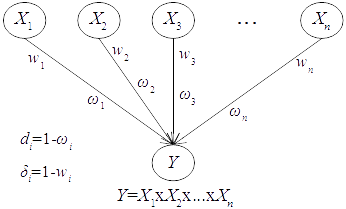
\includegraphics{BiweightSimpleGraph.png}
\caption{Bi-weight simple graph}
\label{figure:biweight-simple-graph}
\end{figure}
%Figure 3.3. Bi-weight simple graph

With bi-weight simple graph, all X-gate inferences are extended as so-called X-gate bi-inferences. Derived from formula~\ref{formula:accountable-probs}, formula~\ref{formula:accountable-probs-biweight} specifies conditional probability of accountable variables with regard to bi-weight graph.

\begin{equation}
\begin{split}
&P\left(A_i=ON\mathrel{\left|\vphantom{A_i=ON X_i=1}\right.\kern-\nulldelimiterspace}X_i=1\right)=p_i=w_i\\
&P\left(A_i=ON\mathrel{\left|\vphantom{A_i=ON X_i=0}\right.\kern-\nulldelimiterspace}X_i=0\right)=1-{\rho }_i=1-{\omega }_i\\
&P\left(A_i=OFF\mathrel{\left|\vphantom{A_i=OFF X_i=1}\right.\kern-\nulldelimiterspace}X_i=1\right)=1-p_i=1-w_i\\
&P\left(A_i=OFF\mathrel{\left|\vphantom{A_i=OFF X_i=0}\right.\kern-\nulldelimiterspace}X_i=0\right)={\rho }_i={\omega }_i\\
\end{split}
\label{formula:accountable-probs-biweight}
\end{equation}
%Formula 3.20. Conditional probability of accountable variables with regard to bi-weight graph

The probabilities \textit{P}(\textit{A${}_{i}$}=\textit{ON} {\textbar} \textit{X${}_{i}$}=0) and \textit{P}(\textit{A${}_{i}$}=\textit{OFF} {\textbar} \textit{X${}_{i}$}=1) are called clockwise adder \textit{d${}_{i}$} and counterclockwise adder \textit{$\delta$${}_{i}$}. As usual, \textit{d${}_{i}$} and \textit{$\delta$${}_{i}$} are smaller than \textit{w${}_{i}$} and \textit{$\omega$${}_{i}$}. When \textit{d${}_{i}$}=0, bi-weight graph becomes normal simple graph.
\begin{align*}
&d_i=P\left(A_i=ON\mathrel{\left|\vphantom{A_i=ON X_i=0}\right.\kern-\nulldelimiterspace}X_i=0\right)=1-{\rho }_i=1-{\omega }_i\\
&{\delta }_i=P\left(A_i=OFF\mathrel{\left|\vphantom{A_i=OFF X_i=1}\right.\kern-\nulldelimiterspace}X_i=1\right)=1-p_i=1-w_i
\end{align*}
The total clockwise weight or total counterclockwise weight is defined as sum of clockwise weight and clockwise adder or sum of counterclockwise weight and counterclockwise adder. Formula~\ref{formula:total-clockwise-counterclockwise} specifies such total weights \textit{W${}_{i}$} and ${\mathcal{W}}_i$. These weights are also called relationship powers.

\begin{equation}
\begin{split}
&W_i=w_i+d_i\\
&{\mathcal{W}}_i={\omega }_i+{\delta }_i\\
&\mathrm{Where,}\\
&d_i=1-{\rho }_i=1-{\omega }_i\\
&{\delta }_i=1-p_i=1-w_i
\end{split}
\label{formula:total-clockwise-counterclockwise}
\end{equation}
%Formula 3.21. Total clockwise and counterclockwise weights

Given formula~\ref{formula:total-clockwise-counterclockwise}, the set of all \textit{A${}_{i}$} (s) is complete if and only if $\sum^n_{i=1}{W_i}=1$.

By extending aforementioned X-gate inferences, we get bi-inferences for AND-gate, OR-gate, NAND-gate, NOR-gate, XOR-gate, XNOR-gate, and U-gate as shown in table~\ref{table:bi-inferences}.

\begin{table}
\centering
\caption{Bi-inferences for AND-gate, OR-gate, NAND-gate, NOR-gate, XOR-gate, XNOR-gate, and U-gate}
\begin{tabular}{|p{\columnwidth}|} \hline
$\begin{aligned}
&P\left(X_1\odot X_2\odot \dots \odot X_n\right)=\prod_{i\in K}{p_i}\prod_{i\in L}{d_i}\\
&P\left(X_1\oplus X_2\oplus \dots \oplus X_n\right)=1-\prod_{i\in K}{{\delta }_i}\prod_{i\in L}{{\rho }_i}\\
&P\left(\mathrm{not}\left(X_1\odot X_2\odot \dots \odot X_n\right)\right)=1-\prod_{i\in L}{{\rho }_i}\prod_{i\in K}{{\delta }_i}\\
&P\left(\mathrm{not}\left(X_1\oplus X_2\oplus \dots \oplus X_n\right)\right)=\prod_{i\in L}{d_i}\prod_{i\in K}{p_i}\\
&P\left(X_1\otimes X_2\otimes \dots \otimes X_n\right)=\prod_{i\in O_1}{p_i}\prod_{i\in O_2}{d_i}\prod_{i\in E_1}{{\delta }_i}\prod_{i\in E_2}{{\rho }_i}\\
&+\prod_{i\in E_1}{p_i}\prod_{i\in E_2}{d_i}\prod_{i\in O_1}{{\delta }_i}\prod_{i\in O_2}{{\rho }_i}\\
\\
&P\left(\mathrm{not}\left(X_1\otimes X_2\otimes \dots \otimes X_n\right)\right)=\prod_{i\in K}{p_i}\prod_{i\in L}{d_i}+\prod_{i\in K}{{\delta }_i}\prod_{i\in L}{{\rho }_i}\\
&P\left(X_1\uplus X_2\uplus \dots \uplus X_n\right)=\sum_{U\in \mathcal{U}}{\left(\prod_{i\in U\cap K}{p_i}\prod_{i\in U\cap L}{d_i}\right)\left(\prod_{i\in \overline{U}\cap K}{{\delta }_i}\prod_{i\in \overline{U}\cap L}{{\rho }_i}\right)}
\end{aligned}$\\
\\There are four common conditions of \textit{U}: {\textbar}\textit{U}{\textbar}=\textit{$\alpha$}, {\textbar}\textit{U}{\textbar}$\mathrm{\ge}$\textit{$\alpha$}, {\textbar}\textit{U}{\textbar}$\mathrm{\le}$\textit{$\beta$}, and \textit{$\alpha$}$\mathrm{\le}${\textbar}\textit{U}{\textbar}$\mathrm{\le}$\textit{$\beta$}. Note that $\overline{U}$ is the complement of \textit{U},\\
$\overline{U}=\left\{1,2,\dots ,n\right\}\backslash U$\\
The largest cardinality of $\mathcal{U}$ is $\left|\mathcal{U}\right|=2^n$
\\ \hline 
\end{tabular}
\label{table:bi-inferences}
\end{table}
%Table 3.3. Bi-inferences for AND-gate, OR-gate, NAND-gate, NOR-gate, XOR-gate, XNOR-gate, and U-gate

The largest cardinalities of \textit{K} (\textit{L}) are 2\textit{${}^{n}$}${}^{-1}$ and 2\textit{${}^{n}$} with and without fixed \textit{X${}_{i}$}. Thus, it is possible to calculate arrangement counters. As a convention, the product of probabilities is 1 if indices set is empty.
\[\prod_{i\in I}{f_i}=1\ \mathrm{if}\ I=\emptyset \] 
With regard to SIGMA-gate bi-inference, the sum of all total clockwise weights must be 1 as follows:
\[\sum^n_{i=1}{W_i}=\sum^n_{i=1}{\left(w_i+d_i\right)}=\sum^n_{i=1}{\left(w_i+1-{\omega }_i\right)}=1\] 
Derived from formula~\ref{sigma-gate-inference}, the SIGMA-gate probability for bi-weight graph is:
\begin{align*}
&P\left(X_1+X_2+\dots +X_n\right)=\sum^n_{i=1}{P\left(A_i=ON\mathrel{\left|\vphantom{A_i=ON X_i}\right.\kern-\nulldelimiterspace}X_i\right)}\\
&=\sum_{i\in K}{P\left(A_i=ON\mathrel{\left|\vphantom{A_i=ON X_i=1}\right.\kern-\nulldelimiterspace}X_i=1\right)}+\sum_{i\in L}{P\left(A_i=ON\mathrel{\left|\vphantom{A_i=ON X_i=0}\right.\kern-\nulldelimiterspace}X_i=0\right)}\\
&=\sum_{i\in K}{w_i}+\sum_{i\in L}{d_i}
\end{align*}
Shortly, formula~\ref{formula:sigma-gate-biinference} specifies SIGMA-gate bi-inference.

\begin{equation}
\begin{split}
&P\left(X_1+X_2+\dots +X_n\right)=\sum_{i\in K}{w_i}+\sum_{i\in L}{d_i}\\
&\mathrm{Where}\ \mathrm{the}\ \mathrm{set}\ \mathrm{of}\ X_i\ \mathrm{(s)}\ \mathrm{is}\ \mathrm{complete}\ \mathrm{and}\ \mathrm{mutually}\ \mathrm{exclusive.}\\
&\sum^n_{i=1}{W_i}=1\\
&X_i\cap X_j=\emptyset ,\forall i\neq j
\end{split}
\label{formula:sigma-gate-biinference}
\end{equation}
%Formula 3.22. SIGMA-gate bi-inference

The next section will research diagnostic relationship which adheres to X-gate inference.

\section{Multi-hypothesis diagnostic relationship}
Given a simple graph shown in figure~\ref{figure:simple-graph}, if we replace the target source \textit{Y} by an evidence \textit{D}, we get a so-called \textit{multi-hypothesis diagnostic relationship} whose property adheres to X-gate inference. Maybe there are other diagnostic relationships in which X-gate inference is not concerned. However, this research focuses on X-gate inference and so multi-hypothesis diagnostic relationship is called \textit{X-gate diagnostic relationship}. Sources \textit{X}${}_{1}$, \textit{X}${}_{2}$,{\dots}, \textit{X${}_{n}$} become hypotheses\textit{.} As a convention, these hypotheses have prior uniform distribution.

According to aforementioned X-gate network shown in figures \ref{figure:simple-graph} and \ref{figure:extended-x-gate-network}, the target variable must be binary whereas evidence \textit{D} can be numeric. It is impossible to establish the evidence \textit{D} as direct target variable. Thus, the solution of this problem is to add an augmented target binary variable \textit{Y} and then, the evidence \textit{D} is connected directly to \textit{Y}. In other words, the \textit{X-gate diagnostic network} have \textit{n} sources $\{$\textit{X}${}_{1}$, \textit{X}${}_{2}$,{\dots}, \textit{X${}_{n}$}$\}$, one augmented hypothesis \textit{Y}, and one evidence \textit{D}. As a convention, X-gate diagnostic network is called \textit{X-D network}. The CPT (s) of the entire network are determined based on combination of diagnostic relationship and X-gate inference mentioned in previous sections. Figure~\ref{figure:augmented-xd-network} depicts the augmented X-D network. Note that variables \textit{X}${}_{1}$, \textit{X}${}_{2}$,{\dots}, \textit{X${}_{n}$}, and \textit{Y} are always binary.

\begin{figure}
\centering
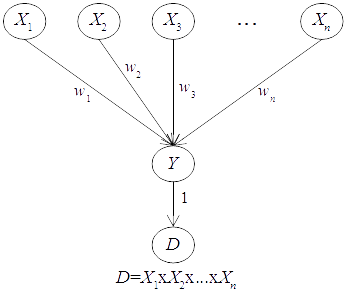
\includegraphics{XDNetwork.png}
\caption{Augmented X-D network}
\label{figure:augmented-xd-network}
\end{figure}
%Figure 4.1. Augmented X-D network

\noindent The joint probability of augmented X-D network shown in figure~\ref{figure:augmented-xd-network} is
\[P\left(X_1,X_2,\dots ,X_n,Y,D\right)=P\left(D\mathrel{\left|\vphantom{D Y}\right.\kern-\nulldelimiterspace}Y\right)P\left(Y\mathrel{\left|\vphantom{Y X_1,X_2,\dots ,X_n}\right.\kern-\nulldelimiterspace}X_1,X_2,\dots ,X_n\right)\prod^n_{i=1}{P\left(X_i\right)}\] 
The joint probability of X-D network is
\[P\left(X_1,X_2,\dots ,X_n,D\right)=P\left(D\mathrel{\left|\vphantom{D X_1,X_2,\dots ,X_n}\right.\kern-\nulldelimiterspace}X_1,X_2,\dots ,X_n\right)\prod^n_{i=1}{P\left(X_i\right)}\] 
By applying total probability rule into X-D network, we have:
\begin{align*}
&P\left(X_1,X_2,\dots ,X_n,D\right)=\frac{P\left(D,X_1,X_2,\dots ,X_n\right)}{P\left(X_1,X_2,\dots ,X_n\right)}\prod^n_{i=1}{P\left(X_i\right)}\\
&\left(\mathrm{Due}\ \mathrm{to}\ \mathrm{Bayes'}\ \mathrm{rule}\right)\\
&=\frac{\sum_Y{P\left(D,X_1,X_2,\dots ,X_n\mathrel{\left|\vphantom{D,X_1,X_2,\dots ,X_n Y}\right.\kern-\nulldelimiterspace}Y\right)P\left(Y\right)}}{P\left(X_1,X_2,\dots ,X_n\right)}\prod^n_{i=1}{P\left(X_i\right)}\\
&\left(\mathrm{Due}\ \mathrm{to}\ \mathrm{total}\ \mathrm{probability}\ \mathrm{rule}\right)\\
&=\frac{\sum_Y{P\left(D,X_1,X_2,\dots ,X_n\mathrel{\left|\vphantom{D,X_1,X_2,\dots ,X_n Y}\right.\kern-\nulldelimiterspace}Y\right)P\left(Y\right)}}{P\left(X_1,X_2,\dots ,X_n\right)}\prod^n_{i=1}{P\left(X_i\right)}\\
&=\left(\sum_Y{P\left(D,X_1,X_2,\dots ,X_n\mathrel{\left|\vphantom{D,X_1,X_2,\dots ,X_n Y}\right.\kern-\nulldelimiterspace}Y\right)*\frac{P\left(Y\right)}{P\left(X_1,X_2,\dots ,X_n\right)}}\right)*\prod^n_{i=1}{P\left(X_i\right)}\\
&=\left(\sum_Y{P\left(D\mathrel{\left|\vphantom{D Y}\right.\kern-\nulldelimiterspace}Y\right)*\frac{P\left(X_1,X_2,\dots ,X_n\mathrel{\left|\vphantom{X_1,X_2,\dots ,X_n Y}\right.\kern-\nulldelimiterspace}Y\right)P\left(Y\right)}{P\left(X_1,X_2,\dots ,X_n\right)}}\right)*\prod^n_{i=1}{P\left(X_i\right)}\\
&\left(\mathrm{Because}\ D\ \mathrm{is}\ \mathrm{conditionally}\ \mathrm{independent}\ \mathrm{from}\ \mathrm{all}\ X_i\ \mathrm{(s)}\ \mathrm{given}\ Y\right)\\
&=\left(\sum_Y{P\left(D\mathrel{\left|\vphantom{D Y}\right.\kern-\nulldelimiterspace}Y\right)*\frac{P\left(Y,X_1,X_2,\dots ,X_n\right)}{P\left(X_1,X_2,\dots ,X_n\right)}}\right)*\prod^n_{i=1}{P\left(X_i\right)}\\
&=\sum_Y{P\left(D\mathrel{\left|\vphantom{D Y}\right.\kern-\nulldelimiterspace}Y\right)P\left(Y\mathrel{\left|\vphantom{Y X_1,X_2,\dots ,X_n}\right.\kern-\nulldelimiterspace}X_1,X_2,\dots ,X_n\right)\prod^n_{i=1}{P\left(X_i\right)}}\\
&\left(\mathrm{Due}\ \mathrm{to}\ \mathrm{Bayes'}\ \mathrm{rule}\right)\\
&=\sum_Y{P\left(X_1,X_2,\dots ,X_n,Y,D\right)}
\end{align*}
It is implied that the augmented X-D network is equivalent to X-D network with regard to variables \textit{X}${}_{1}$, \textit{X}${}_{2}$,{\dots}, \textit{X${}_{n}$} and \textit{D}. As a convention, augmented X-D network is considered as same as X-D network.

The simplest case of X-D network is NOT-D network having one hypothesis \textit{X}${}_{1}$ and one evidence \textit{D}, equipped with NOT-gate inference. NOT-D network satisfies diagnostic condition because it essentially represents the single diagnostic relationship. Inferred from formulas \ref{formula:cpt-evidence-diagnostic} and \ref{formula:not-gate-inference}, the conditional probability \textit{P}(\textit{D{\textbar}X}${}_{1}$) and posterior probability \textit{P}(\textit{X}${}_{1}$\textit{{\textbar}D}) of NOT-D network are:
\[P\left(D\mathrel{\left|\vphantom{D X_1}\right.\kern-\nulldelimiterspace}X_1\right)=\left\{ \begin{array}{r}
1-D\ \mathrm{if}\ X_1=1 \\ 
D\ \mathrm{if}\ X_1=0 \end{array}
\right.\] 

\begin{align*}
&P\left(X_1\mathrel{\left|\vphantom{X_1 D}\right.\kern-\nulldelimiterspace}D\right)=\frac{P\left(D\mathrel{\left|\vphantom{D X_1}\right.\kern-\nulldelimiterspace}X_1\right)P\left(X_1\right)}{P\left(X_1\right)\left(P\left(D\mathrel{\left|\vphantom{D X_1=0}\right.\kern-\nulldelimiterspace}X_1=0\right)+P\left(D\mathrel{\left|\vphantom{D X_1=1}\right.\kern-\nulldelimiterspace}X_1=1\right)\right)}\\
&\left(\mathrm{Due}\ \mathrm{to}\ \mathrm{Bayes'}\ \mathrm{rule}\ \mathrm{and}\ \mathrm{uniform}\ \mathrm{distribution}\ \mathrm{of}\ X_1\right)\\
&=\frac{P\left(D\mathrel{\left|\vphantom{D X_1}\right.\kern-\nulldelimiterspace}X_1\right)}{P\left(D\mathrel{\left|\vphantom{D X_1=0}\right.\kern-\nulldelimiterspace}X_1=0\right)+P\left(D\mathrel{\left|\vphantom{D X_1=1}\right.\kern-\nulldelimiterspace}X_1=1\right)}=1*P\left(D\mathrel{\left|\vphantom{D X_1}\right.\kern-\nulldelimiterspace}X_1\right)\\
&\left(\mathrm{due\ to}\ P\left(D\mathrel{\left|\vphantom{D X_1=0}\right.\kern-\nulldelimiterspace}X_1=0\right)+P\left(D\mathrel{\left|\vphantom{D X_1=1}\right.\kern-\nulldelimiterspace}X_1=1\right)=1\right)
\end{align*}
It implies NOT-D network satisfies diagnostic condition. Let
\begin{align*}
\Omega&=\left\{X_1,X_2,\dots ,X_n\right\}\\
n&=\left|\Omega\right|
\end{align*}
We will validate whether the CPT of diagnostic relationship, \textit{P}(\textit{D{\textbar}X}) specified by formula~\ref{formula:cpt-evidence}, still satisfies diagnostic condition within general case, X-D network. In other words, X-D network is general case of single diagnostic relationship.

Recall from dependencies shown in figure~\ref{figure:augmented-xd-network}, formula~\ref{formula:joint-prob-xd-network} specifies the joint probability of X-D network.

\begin{equation}
\begin{split}
P\left(\mathrm{\Omega },Y,D\right)&=P\left(X_1,X_2,\dots ,X_n,Y,D\right)\\
&=P\left(D\mathrel{\left|\vphantom{D Y}\right.\kern-\nulldelimiterspace}Y\right)P\left(Y\mathrel{\left|\vphantom{Y X_1,X_2,\dots ,X_n}\right.\kern-\nulldelimiterspace}X_1,X_2,\dots ,X_n\right)\prod^n_{i=1}{P\left(X_i\right)}
\end{split}
\label{formula:joint-prob-xd-network}
\end{equation}
\[\mathrm{Where}\ \Omega=\left\{X_1,X_2,\dots,X_n\right\}\mathrm{.}\]
%Formula 4.1. Joint probability of X-D network

\noindent Formula~\ref{formula:general-cond-prob} specifies the conditional probability of \textit{D} given \textit{X${}_{i}$} (likelihood function) and the posterior probability of \textit{X${}_{i}$} given \textit{D}.

\begin{equation}
\begin{split}
&P\left(D\mathrel{\left|\vphantom{D X_i}\right.\kern-\nulldelimiterspace}X_i\right)=\frac{P\left(X_i,D\right)}{P\left(X_i\right)}=\frac{\sum_{\left\{\mathrm{\Omega },Y,D\right\}\backslash \left\{X_i,D\right\}}{P\left(\mathrm{\Omega },Y,D\right)}}{\sum_{\left\{\mathrm{\Omega },Y,D\right\}\backslash \left\{X_i\right\}}{P\left(\mathrm{\Omega },Y,D\right)}}\\
&P\left(X_i\mathrel{\left|\vphantom{X_i D}\right.\kern-\nulldelimiterspace}D\right)=\frac{P\left(X_i,D\right)}{P\left(D\right)}=\frac{\sum_{\left\{\mathrm{\Omega },Y,D\right\}\backslash \left\{X_i,D\right\}}{P\left(\mathrm{\Omega },Y,D\right)}}{\sum_{\left\{\mathrm{\Omega },Y,D\right\}\backslash \left\{D\right\}}{P\left(\mathrm{\Omega },Y,D\right)}}
\end{split}
\label{formula:general-cond-prob}
\end{equation}
Where $\Omega$ = $\{$\textit{X}${}_{1}$, \textit{X}${}_{2}$,{\dots}, \textit{X${}_{n}$}$\}$ and the sign  ``{\textbackslash}''  denotes  the  subtraction  (excluding)  operator in  set  theory \cite{wikipedia:set}.
%Formula 4.2. Conditional probability \textit{P}(\textit{D}{\textbar}\textit{X${}_{i}$}) and posterior probability \textit{P}(\textit{X${}_{i}$}{\textbar}\textit{D})

Given uniform distribution of \textit{X${}_{i}$} (s), we have:
\[P\left(X_1\right)=P\left(X_2\right)=\cdots =P\left(X_n\right)=\frac{1}{2}\] 
The joint probability becomes
\[P\left(\mathrm{\Omega },Y,D\right)=\frac{1}{2^n}P\left(Y\mathrel{\left|\vphantom{Y X_1,X_2,\dots ,X_n}\right.\kern-\nulldelimiterspace}X_1,X_2,\dots ,X_n\right)P\left(D\mathrel{\left|\vphantom{D Y}\right.\kern-\nulldelimiterspace}Y\right)\] 
The joint probability of \textit{X${}_{i}$} and \textit{D} is:
\begin{align*}
&P\left(X_i,D\right)=\sum_{\left\{\mathrm{\Omega },Y,D\right\}\backslash \left\{X_i,D\right\}}{P\left(\mathrm{\Omega },Y,D\right)}\\
&=P\left(X_1=1,X_2=1,\dots ,X_i,\dots ,X_{n-1}=1,X_n=1,Y=1,D\right)\\
&+P\left(X_1=1,X_2=1,\dots ,X_i,\dots ,X_{n-1}=1,X_n=0,Y=1,D\right)\\
&+\cdots \\
&+P\left(X_1=0,X_2=0,\dots ,X_i,\dots ,X_{n-1}=0,X_n=1,Y=1,D\right)\\
&+P\left(X_1=0,X_2=0,\dots ,X_i,\dots ,X_{n-1}=0,X_n=0,Y=1,D\right)\\
&+P\left(X_1=1,X_2=1,\dots ,X_i,\dots ,X_{n-1}=1,X_n=1,Y=0,D\right)\\
&+P\left(X_1=1,X_2=1,\dots ,X_i,\dots ,X_{n-1}=1,X_n=0,Y=0,D\right)\\
&+\cdots \\
&+P\left(X_1=0,X_2=0,\dots ,X_i,\dots ,X_{n-1}=0,X_n=1,Y=0,D\right)\\
&+P\left(X_1=0,X_2=0,\dots ,X_i,\dots ,X_{n-1}=0,X_n=0,Y=0,D\right)\\
&=\frac{1}{2^n}\frac{D}{S}\left(P\left(Y=1\mathrel{\left|\vphantom{Y=1 X_1=1,X_2=1,\dots ,X_i,\dots ,X_{n-1}=1,X_n=1}\right.\kern-\nulldelimiterspace}X_1=1,X_2=1,\dots ,X_i,\dots ,X_{n-1}=1,X_n=1\right)\right)\\
&+\frac{1}{2^n}\frac{D}{S}\left(P\left(Y=1\mathrel{\left|\vphantom{Y=1 X_1=1,X_2=1,\dots ,X_i,\dots ,X_{n-1}=1,X_n=0}\right.\kern-\nulldelimiterspace}X_1=1,X_2=1,\dots ,X_i,\dots ,X_{n-1}=1,X_n=0\right)\right)\\
&+\cdots \\
&+\frac{1}{2^n}\frac{D}{S}\left(P\left(Y=1\mathrel{\left|\vphantom{Y=1 X_1=1,X_2=1,\dots ,X_i,\dots ,X_{n-1}=0,X_n=1}\right.\kern-\nulldelimiterspace}X_1=1,X_2=1,\dots ,X_i,\dots ,X_{n-1}=0,X_n=1\right)\right)\\
&+\frac{1}{2^n}\frac{D}{S}\left(P\left(Y=1\mathrel{\left|\vphantom{Y=1 X_1=1,X_2=1,\dots ,X_i,\dots ,X_{n-1}=0,X_n=0}\right.\kern-\nulldelimiterspace}X_1=1,X_2=1,\dots ,X_i,\dots ,X_{n-1}=0,X_n=0\right)\right)\\
&+\frac{1}{2^n}\frac{M-D}{S}\left(P\left(Y=0\mathrel{\left|\vphantom{Y=0 X_1=1,X_2=1,\dots ,X_i,\dots ,X_{n-1}=1,X_n=1}\right.\kern-\nulldelimiterspace}X_1=1,X_2=1,\dots ,X_i,\dots ,X_{n-1}=1,X_n=1\right)\right)\\
&+\frac{1}{2^n}\frac{M-D}{S}\left(P\left(Y=0\mathrel{\left|\vphantom{Y=0 X_1=1,X_2=1,\dots ,X_i,\dots ,X_{n-1}=1,X_n=0}\right.\kern-\nulldelimiterspace}X_1=1,X_2=1,\dots ,X_i,\dots ,X_{n-1}=1,X_n=0\right)\right)\\
&+\cdots \\
&+\frac{1}{2^n}\frac{M-D}{S}\left(P\left(Y=0\mathrel{\left|\vphantom{Y=0 X_1=1,X_2=1,\dots ,X_i,\dots ,X_{n-1}=0,X_n=1}\right.\kern-\nulldelimiterspace}X_1=1,X_2=1,\dots ,X_i,\dots ,X_{n-1}=0,X_n=1\right)\right)\\
&+\frac{1}{2^n}\frac{M-D}{S}\left(P\left(Y=0\mathrel{\left|\vphantom{Y=0 X_1=1,X_2=1,\dots ,X_i,\dots ,X_{n-1}=0,X_n=0}\right.\kern-\nulldelimiterspace}X_1=1,X_2=1,\dots ,X_i,\dots ,X_{n-1}=0,X_n=0\right)\right)\\
&\left(\mathrm{Due\ to\ formula\ \ref{formula:cpt-evidence}}\right)
\end{align*}

The marginal probability of \textit{D} is:
\begin{align*}
&P\left(D\right)=\sum_{\left\{\mathrm{\Omega },Y,D\right\}\backslash \left\{D\right\}}{P\left(\mathrm{\Omega },Y,D\right)}\\
&=P\left(X_1=1,X_2=1,\dots ,X_n=1,Y=1,D\right)\\
&+P\left(X_1=1,X_2=1,\dots ,X_n=0,Y=1,D\right)+\cdots \\
&+P\left(X_1=0,X_2=0,\dots ,X_n=1,Y=1,D\right)\\
&+P\left(X_1=0,X_2=0,\dots ,X_n=0,Y=1,D\right)\\
&+P\left(X_1=1,X_2=1,\dots ,X_n=1,Y=0,D\right)\\
&+P\left(X_1=1,X_2=1,\dots ,X_n=0,Y=0,D\right)+\cdots \\
&+P\left(X_1=0,X_2=0,\dots ,X_n=1,Y=0,D\right)\\
&+P\left(X_1=0,X_2=0,\dots ,X_n=0,Y=0,D\right)\\
&=\frac{1}{2^n}\frac{D}{S}\left(P\left(Y=1\mathrel{\left|\vphantom{Y=1 X_1=1,X_2=1,\dots ,X_n=1}\right.\kern-\nulldelimiterspace}X_1=1,X_2=1,\dots ,X_n=1\right)\right)\\
&+\frac{1}{2^n}\frac{D}{S}\left(P\left(Y=1\mathrel{\left|\vphantom{Y=1 X_1=1,X_2=1,\dots ,X_n=0}\right.\kern-\nulldelimiterspace}X_1=1,X_2=1,\dots ,X_n=0\right)\right)+\cdots \\
&+\frac{1}{2^n}\frac{D}{S}\left(P\left(Y=1\mathrel{\left|\vphantom{Y=1 X_1=1,X_2=1,\dots ,X_n=1}\right.\kern-\nulldelimiterspace}X_1=1,X_2=1,\dots ,X_n=1\right)\right)\\
&+\frac{1}{2^n}\frac{D}{S}\left(P\left(Y=1\mathrel{\left|\vphantom{Y=1 X_1=1,X_2=1,\dots ,X_n=0}\right.\kern-\nulldelimiterspace}X_1=1,X_2=1,\dots ,X_n=0\right)\right)\\
&+\frac{1}{2^n}\frac{M-D}{S}\left(P\left(Y=0\mathrel{\left|\vphantom{Y=0 X_1=1,X_2=1,\dots ,X_n=1}\right.\kern-\nulldelimiterspace}X_1=1,X_2=1,\dots ,X_n=1\right)\right)\\
&+\frac{1}{2^n}\frac{M-D}{S}\left(P\left(Y=0\mathrel{\left|\vphantom{Y=0 X_1=1,X_2=1,\dots ,X_n=0}\right.\kern-\nulldelimiterspace}X_1=1,X_2=1,\dots ,X_n=0\right)\right)+\cdots \\
&+\frac{1}{2^n}\frac{M-D}{S}\left(P\left(Y=0\mathrel{\left|\vphantom{Y=0 X_1=1,X_2=1,\dots ,X_n=1}\right.\kern-\nulldelimiterspace}X_1=1,X_2=1,\dots ,X_n=1\right)\right)\\
&+\frac{1}{2^n}\frac{M-D}{S}\left(P\left(Y=0\mathrel{\left|\vphantom{Y=0 X_1=1,X_2=1,\dots ,X_n=0}\right.\kern-\nulldelimiterspace}X_1=1,X_2=1,\dots ,X_n=0\right)\right)
\end{align*}
By applying definition~\ref{definition:binary-arrangements}, the joint probability \textit{P}(\textit{X${}_{i}$}, \textit{D}) is determined as follows:
\begin{align*}
&P\left(X_i,D\right)\\
&=\frac{1}{2^nS}\left(D\sum_a{P\left(Y=1\mathrel{\left|\vphantom{Y=1 a\left(\mathrm{\Omega }\mathrm{:}\left\{X_i\right\}\right)}\right.\kern-\nulldelimiterspace}a\left(\mathrm{\Omega }\mathrm{:}\left\{X_i\right\}\right)\right)}+\left(M-D\right)\sum_a{P\left(Y=0\mathrel{\left|\vphantom{Y=0 a\left(\mathrm{\Omega }\mathrm{:}\left\{X_i\right\}\right)}\right.\kern-\nulldelimiterspace}a\left(\mathrm{\Omega }\mathrm{:}\left\{X_i\right\}\right)\right)}\right)\\
&=\frac{1}{2^nS}\left(D\sum_a{P\left(Y=1\mathrel{\left|\vphantom{Y=1 a\left(\mathrm{\Omega }\mathrm{:}\left\{X_i\right\}\right)}\right.\kern-\nulldelimiterspace}a\left(\mathrm{\Omega }\mathrm{:}\left\{X_i\right\}\right)\right)}+\left(M-D\right)\sum_a{\left(1-P\left(Y=1\mathrel{\left|\vphantom{Y=1 a\left(\mathrm{\Omega }\mathrm{:}\left\{X_i\right\}\right)}\right.\kern-\nulldelimiterspace}a\left(\mathrm{\Omega }\mathrm{:}\left\{X_i\right\}\right)\right)\right)}\right)\\
&=\frac{1}{2^nS}\left(\left(2D-M\right)s\left(\mathrm{\Omega }\mathrm{:}\left\{X_i\right\}\right)+2^{n-1}\left(M-D\right)\right)
\end{align*}
Similarly, formula~\ref{formula:join-marginal-probs} specifies the joint probability \textit{P}(\textit{X${}_{i}$}, \textit{D}) and the marginal probability \textit{P}(\textit{D}) given uniform distribution of all sources.

\begin{equation}
\begin{split}
&P\left(X_i,D\right)=\frac{1}{2^nS}\left(\left(2D-M\right)s\left(\mathrm{\Omega }\mathrm{:}\left\{X_i\right\}\right)+2^{n-1}\left(M-D\right)\right)\\
&P\left(D\right)=\frac{1}{2^nS}\left(\left(2D-M\right)s\left(\mathrm{\Omega }\right)+2^n\left(M-D\right)\right)
\end{split}
\label{formula:join-marginal-probs}
\end{equation}
%Formula 4.3. Joint probability \textit{P}(\textit{X${}_{i}$}, \textit{D}) and marginal probability \textit{P}(\textit{D}) given uniform distribution of all sources
Where \textit{s}($\Omega$) and \textit{s}($\Omega$:$\{$\textit{X${}_{i}$}$\}$) are specified in definition~\ref{definition:binary-arrangements}.

In general, formula~\ref{formula:join-marginal-probs-xd-network} specifies conditional probability \textit{P}(\textit{D{\textbar}X${}_{i}$}), posterior probability \textit{P}(\textit{X${}_{i}${\textbar}D}), and transformation coefficient for X-gate inference.

\begin{equation}
\begin{split}
P\left(D\mathrel{\left|\vphantom{D X_i=1}\right.\kern-\nulldelimiterspace}X_i=1\right)&=\frac{P\left(X_i=1,D\right)}{P\left(X_i=1\right)}\\
&=\frac{\left(2D-M\right)s\left(\mathrm{\Omega }\mathrm{:}\left\{X_i=1\right\}\right)+2^{n-1}\left(M-D\right)}{2^{n-1}S}\\
P\left(D\mathrel{\left|\vphantom{D X_i=0}\right.\kern-\nulldelimiterspace}X_i=0\right)&=\frac{P\left(X_i=0,D\right)}{P\left(X_i=0\right)}\\
&=\frac{\left(2D-M\right)s\left(\mathrm{\Omega }\mathrm{:}\left\{X_i=0\right\}\right)+2^{n-1}\left(M-D\right)}{2^{n-1}S}\\
P\left(X_i=1\mathrel{\left|\vphantom{X_i=1 D}\right.\kern-\nulldelimiterspace}D\right)&=\frac{P\left(X_i=1,D\right)}{P\left(D\right)}\\
&=\frac{\left(2D-M\right)s\left(\mathrm{\Omega }\mathrm{:}\left\{X_i=1\right\}\right)+2^{n-1}\left(M-D\right)}{\left(2D-M\right)s\left(\mathrm{\Omega }\right)+2^n\left(M-D\right)}\\
P\left(X_i=0\mathrel{\left|\vphantom{X_i=0 D}\right.\kern-\nulldelimiterspace}D\right)&=1-P\left(X_i=1\mathrel{\left|\vphantom{X_i=1 D}\right.\kern-\nulldelimiterspace}D\right)\\
&=\frac{\left(2D-M\right)s\left(\mathrm{\Omega }\mathrm{:}\left\{X_i=0\right\}\right)+2^{n-1}\left(M-D\right)}{\left(2D-M\right)s\left(\mathrm{\Omega }\right)+2^n\left(M-D\right)}\\
k&=\frac{P\left(X_i\mathrel{\left|\vphantom{X_i D}\right.\kern-\nulldelimiterspace}D\right)}{P\left(D\mathrel{\left|\vphantom{D X_i}\right.\kern-\nulldelimiterspace}X_i\right)}=\frac{2^{n-1}S}{\left(2D-M\right)s\left(\mathrm{\Omega }\right)+2^n\left(M-D\right)}
\end{split}
\label{formula:join-marginal-probs-xd-network}
\end{equation}
%Formula 4.4. Conditional probability, posterior probability, and transformation coefficient of X-D network

\noindent The transformation coefficient is rewritten as follows:
\[k=\frac{2^{n-1}S}{2D\left(s\left(\mathrm{\Omega }\right)-2^{n-1}\right)+M\left(2^n-s\left(\mathrm{\Omega }\right)\right)}\] 
Note that \textit{S}, \textit{D}, \textit{M} are abstract symbols and there is no proportional connection between 2\textit{${}^{n}$}${}^{-1}$\textit{S} and \textit{D} for all \textit{D}, specified by formula~\ref{formula:cpt-evidence}. Assuming that such proportional connection 2\textit{${}^{n}$}${}^{-1}$\textit{S} = \textit{aD${}^{j}$} exists for all \textit{D} where \textit{a} is arbitrary constant. Given binary case when \textit{D}=0 and \textit{S}=1, we have:
\[2^{n-1}=2^{n-1}*1=2^{n-1}S=aD^j=a*0^j=0\] 
There is a contradiction, which implies that it is impossible to reduce \textit{k} into the following form:
\[k=\frac{aD^j}{bD^j}\]
Therefore, if \textit{k} is constant with regard to \textit{D} then,
\[2D\left(s\left(\mathrm{\Omega }\right)-2^{n-1}\right)+M\left(2^n-s\left(\mathrm{\Omega }\right)\right)=C\neq 0,\forall D\] 
Where \textit{C} is constant. We have:
\begin{align*}
&\sum_D{\left(2D\left(s\left(\mathrm{\Omega }\right)-2^{n-1}\right)+M\left(2^n-s\left(\mathrm{\Omega }\right)\right)\right)}=\sum_D{C}\\
&\Rightarrow 2S\left(s\left(\mathrm{\Omega }\right)-2^{n-1}\right)+NM\left(2^n-s\left(\mathrm{\Omega }\right)\right)=NC\\
&\Rightarrow 2^nS=NC
\end{align*}
It is implied that
\begin{align*}
k&=\frac{2^{n-1}S}{2D\left(s\left(\mathrm{\Omega }\right)-2^{n-1}\right)+M\left(2^n-s\left(\mathrm{\Omega }\right)\right)}\\
&=\frac{NC}{2C}=\frac{N}{2}
\end{align*}
This holds
\begin{align*}
&2^nS=N\left(2D\left(s\left(\mathrm{\Omega }\right)-2^{n-1}\right)+M\left(2^n-s\left(\mathrm{\Omega }\right)\right)\right)\\
&\Rightarrow 2^nS=2ND\left(s\left(\mathrm{\Omega }\right)-2^{n-1}\right)+2S\left(2^n-s\left(\mathrm{\Omega }\right)\right)\\
&\Rightarrow 2ND\left(s\left(\mathrm{\Omega }\right)-2^{n-1}\right)-2S\left(s\left(\mathrm{\Omega }\right)-2^{n-1}\right)=0\\
&\Rightarrow \left(ND-S\right)\left(s\left(\mathrm{\Omega }\right)-2^{n-1}\right)=0
\end{align*}
Assuming \textit{ND}=\textit{S} we have:
\[ND=S=2NM\Rightarrow D=2M\] 
There is a contradiction because \textit{M} is maximum value of \textit{D}. Therefore, if \textit{k} is constant with regard to \textit{D} then \textit{s}($\Omega$) = 2\textit{${}^{n}$}${}^{-1}$. Inversely, if \textit{s}($\Omega$) = 2\textit{${}^{n}$}${}^{-1}$ then \textit{k} is:
\[k=\frac{2^{n-1}S}{2D\left(2^{n-1}-2^{n-1}\right)+M\left(2^n-2^{n-1}\right)}=\frac{N}{2}\] 
In general, the event that \textit{k} is constant with regard to \textit{D} is equivalent to the event \textit{s}($\Omega$) = 2\textit{${}^{n}$}${}^{-1}$. In general, diagnostic theorem is stated as follows:

\begin{theorem}[Diagnostic theorem]
The diagnostic condition of X-D network is satisfied if and only if
\begin{center}
$\begin{aligned}
s\left(\mathrm{\Omega }\right)=\sum_a{P\left(Y=1\mathrel{\left|\vphantom{Y=1 a\left(\mathrm{\Omega }\right)}\right.\kern-\nulldelimiterspace}a\left(\mathrm{\Omega }\right)\right)}=2^{\left|\mathrm{\Omega }\right|-1},\forall \mathrm{\Omega }\neq \emptyset
\end{aligned}$
\end{center}
At that time, the transformation coefficient becomes:
\begin{center}
$\begin{aligned}
k=\frac{N}{2}
\end{aligned}$
\end{center}
%\end{tabular}
\label{theorem:diagnostic-theorem}
\end{theorem}

Where the X-D network is combination of diagnostic relationship and X-gate inference as follows:
\begin{align*}
&P\left(Y=1\mathrel{\left|\vphantom{Y=1 X_1,X_2,\dots ,X_n}\right.\kern-\nulldelimiterspace}X_1,X_2,\dots ,X_n\right)=P\left(X_1\mathrm{x}X_2\mathrm{x}\dots \mathrm{x}X_n\right)\\
&P\left(D\mathrel{\left|\vphantom{D Y}\right.\kern-\nulldelimiterspace}Y\right)=\left\{ \begin{array}{r}
\frac{D}{S}\ \mathrm{if}\ Y=1 \\ 
\frac{M}{S}-\frac{D}{S}\ \mathrm{if}\ Y=0 \end{array}
\right.
\end{align*}
Note that weights $p_i=w_i$ and $\rho_i=\omega_i$, which are inputs of $s\left(\Omega\right)$, are abstract variables. Thus, the equality $s\left(\Omega\right)=2^{\left|\Omega\right|-1}$ implies all abstract variables are removed and so $s\left(\Omega\right)$ does not depend on weights. The diagnostic theorem is the optimal way to validate the diagnostic condition.

The formula~\ref{formula:join-marginal-probs-xd-network} becomes simple with AND-gate inference. Recall that formula~\ref{formula:and-gate-inference} specified AND-gate inference as follows:
\begin{align*}
P\left(X_1\odot X_2\odot \dots \odot X_n\right)&=P\left(Y=1\mathrel{\left|\vphantom{Y=1 X_1,X_2,\dots ,X_n}\right.\kern-\nulldelimiterspace}X_1,X_2,\dots ,X_n\right)\\
&=\left\{ \begin{array}{l}
\prod^n_{i=1}{p_i}\ \mathrm{if\ all}\ X_i\ \left(s\right)\ \mathrm{are}\ 1 \\ 
0\ \mathrm{if\ there\ exists\ at\ least\ one\ }X_i=0 \end{array}
\right.
\end{align*}
Due to only one case \textit{X}${}_{1}$ = \textit{X}${}_{2}$ ={\dots}= \textit{X${}_{n}$} = 1, we have:
\[s\left(\mathrm{\Omega }\right)=s\left(\mathrm{\Omega }\mathrm{:}\left\{X_i=1\right\}\right)=\prod^n_{i=1}{p_i}\] 
Due to \textit{X${}_{i}$} = 0, we have:
\[s\left(\mathrm{\Omega }\mathrm{:}\left\{X_i=0\right\}\right)=0\] 
Derived from formula~\ref{formula:join-marginal-probs-xd-network}, formula~\ref{formula:cond-post-prob-andd-network} specifies conditional probability \textit{P}(\textit{D{\textbar}X${}_{i}$}), posterior probability \textit{P}(\textit{X${}_{i}${\textbar}D}), and transformation coefficient according to X-D network with AND-gate reference called \textit{AND-D network}.

\begin{equation}
\begin{split}
&P\left(D\mathrel{\left|\vphantom{D X_i=1}\right.\kern-\nulldelimiterspace}X_i=1\right)=\frac{\left(2D-M\right)\prod^n_{i=1}{p_i}+2^{n-1}\left(M-D\right)}{2^{n-1}S}\\
&P\left(D\mathrel{\left|\vphantom{D X_i=0}\right.\kern-\nulldelimiterspace}X_i=0\right)=\frac{M-D}{S}\\
&P\left(X_i=1\mathrel{\left|\vphantom{X_i=1 D}\right.\kern-\nulldelimiterspace}D\right)=\frac{\left(2D-M\right)\prod^n_{i=1}{p_i}+2^{n-1}\left(M-D\right)}{\left(2D-M\right)\prod^n_{i=1}{p_i}+2^n\left(M-D\right)}\\
&P\left(X_i=0\mathrel{\left|\vphantom{X_i=0 D}\right.\kern-\nulldelimiterspace}D\right)=\frac{2^{n-1}\left(M-D\right)}{\left(2D-M\right)\prod^n_{i=1}{p_i}+2^n\left(M-D\right)}\\
&k=\frac{2^{n-1}S}{\left(2D-M\right)\prod^n_{i=1}{p_i}+2^n\left(M-D\right)}
\end{split}
\label{formula:cond-post-prob-andd-network}
\end{equation}
%Formula 4.5. Conditional probability and posterior probability of AND-D network

For convenience, we validate diagnostic condition with a case of two sources $\Omega$ = $\{$\textit{X}${}_{1}$, \textit{X}${}_{2}$$\}$, \textit{p}${}_{1}$ = \textit{p}${}_{2}$ = \textit{w}${}_{1}$ = \textit{w}${}_{2}$ = 0.5, $D\in \{0,1,2,3\}$. According to diagnostic theorem, if \textit{s}($\Omega$) $\mathrm{\neq}$ 2 for given X-gate then, such X-gate does not satisfy diagnostic condition.

Given AND-gate inference, by applying formula~\ref{formula:and-gate-inference}, we have:
\[s\left(\mathrm{\Omega }\right)=\left(0.5*0.5\right)+0+0+0=0.25\] 
Given OR-gate inference, by applying formula~\ref{formula:or-gate-inference}, we have:
\[s\left(\mathrm{\Omega }\right)=\left(1-0.5*0.5\right)+\left(1-0.5\right)+\left(1-0.5\right)+0=1.75\] 
Given XOR-gate inference, by applying formula~\ref{formula:xor-gate-inference}, we have:
\[s\left(\mathrm{\Omega }\right)=\left(0.5*0.5+0.5*0.5\right)+0.5+0.5+0=1.5\] 
Given XNOR-gate inference, by applying formula~\ref{xnor-gate-inference}, we have:
\[s\left(\mathrm{\Omega }\right)=\left(0.5*0.5+0.5*0.5\right)+0.5+0.5+1=2.5\] 
Given SIGMA-gate inference, by applying formula~\ref{sigma-gate-inference}, we have:
\[s\left(\mathrm{\Omega }\right)=\left(0.5+0.5\right)+0.5+0.5+0=2\] 
It is asserted that AND-gate, OR-gate, XOR-gate, and XNOR-gate do not satisfy diagnostic condition and so they should not be used to assess hypotheses. However, it is not asserted if U-gate and SIGMA-gate satisfy such diagnostic condition. It is necessary to expend formula for SIGMA-gate diagnostic network (called \textit{SIGMA-D network}) in order to validate it.

In case of SIGMA-gate inference, by applying formula~\ref{sigma-gate-inference}, we have:
\begin{align*}
\sum_i{w_i}&=1\\
s\left(\mathrm{\Omega }\right)&=2^{n-1}\sum_i{w_i}=2^{n-1}\\
s\left(\mathrm{\Omega }\mathrm{:}\left\{X_i=1\right\}\right)&=2^{n-1}w_i+2^{n-2}\sum_{j\neq i}{w_j}\\
&=2^{n-1}w_i+2^{n-2}\left(1-w_i\right)=2^{n-2}\left(1+w_i\right)\\
s\left(\mathrm{\Omega }\mathrm{:}\left\{X_i=0\right\}\right)&=s\left(\mathrm{\Omega }\right)-s\left(\mathrm{\Omega }\mathrm{:}\left\{X_i=1\right\}\right)\\
&=2^{n-2}\left(1-w_i\right)
\end{align*}
It is necessary to validate SIGMA-D network with SIGMA-gate bi-inference. By applying formula~\ref{formula:sigma-gate-biinference}, we recalculate these quantities as follows:
\begin{align*}
s\left(\mathrm{\Omega }\right)&=2^{n-1}\sum_i{w_i}+2^{n-1}\sum_i{d_i}=2^{n-1}\sum_i{\left(w_i+d_i\right)}=2^{n-1}\\
&\left(\mathrm{due\ to}\sum_i{\left(w_i+d_i\right)}=1\right)\\
s\left(\mathrm{\Omega }\mathrm{:}\left\{X_i=1\right\}\right)&=2^{n-1}w_i+2^{n-2}\sum_{j\neq i}{w_j}+2^{n-2}\sum_i{d_i}\\
&=2^{n-2}w_i+2^{n-2}\sum_i{\left(w_i+d_i\right)}=2^{n-2}\left(1+w_i\right)\\
s\left(\mathrm{\Omega }\mathrm{:}\left\{X_i=0\right\}\right)&=s\left(\mathrm{\Omega }\right)-s\left(\mathrm{\Omega }\mathrm{:}\left\{X_i=1\right\}\right)=2^{n-2}\left(1-w_i\right)
\end{align*}
Obviously, quantities \textit{s}($\Omega$), \textit{s}($\Omega$:$\{$\textit{X${}_{i}$}=1$\}$), and \textit{s}($\Omega$:$\{$\textit{X${}_{i}$}=0$\}$) are kept intact. According to diagnostic theorem, we conclude that SIGMA-D network does satisfy diagnostic condition due to \textit{s}($\Omega$)=2\textit{${}^{n}$}${}^{--1}$. Thus, SIGMA-D network can be used to assess hypotheses.

Formula~\ref{cond-post-k-sigmad-network}, an immediate consequence of formula~\ref{formula:join-marginal-probs-xd-network}, specifies conditional probability \textit{P}(\textit{D{\textbar}X${}_{i}$}), posterior probability \textit{P}(\textit{X${}_{i}${\textbar}D}), and transformation coefficient for SIGMA-D network.

\begin{equation}
\begin{split}
&P\left(D\mathrel{\left|\vphantom{D X_i=1}\right.\kern-\nulldelimiterspace}X_i=1\right)=\frac{\left(2D-M\right)w_i+M}{2S}\\
&P\left(D\mathrel{\left|\vphantom{D X_i=0}\right.\kern-\nulldelimiterspace}X_i=0\right)=\frac{\left(M-2D\right)w_i+M}{2S}\\
&P\left(X_i=1\mathrel{\left|\vphantom{X_i=1 D}\right.\kern-\nulldelimiterspace}D\right)=\frac{\left(2D-M\right)w_i+M}{2M}\\
&P\left(X_i=0\mathrel{\left|\vphantom{X_i=0 D}\right.\kern-\nulldelimiterspace}D\right)=\frac{\left(M-2D\right)w_i+M}{2M}\\
&k=\frac{N}{2}
\end{split}
\label{cond-post-k-sigmad-network}
\end{equation}
%Formula 4.6. Conditional probability, posterior probability, and transformation coefficient of SIGMA-D network

In case of SIGMA-gate, the augmented variable \textit{Y} can be removed from X-D network. The evidence \textit{D} is now established as direct target variable. Figure~\ref{figure:direct-sigmad-network} shows a so-called \textit{direct SIGMA-gate diagnostic network} (direct SIGMA-D network).

\begin{figure}
\centering
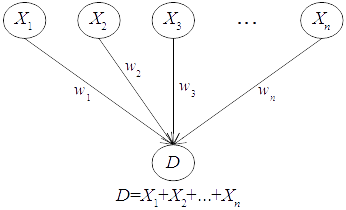
\includegraphics{DirectSIGMADNetwork.png}
\caption{Direct SIGMA-gate diagnostic network (direct SIGMA-D network)}
\label{figure:direct-sigmad-network}
\end{figure}
%Figure 4.2. Direct SIGMA-gate diagnostic network (direct SIGMA-D network)

Derived from formula~\ref{sigma-gate-inference}, the CPT of direct SIGMA-D network is determined by formula~\ref{formula:cpt-direct-sigmad-network}.

\begin{equation}
\begin{split}
&P\left(D\mathrel{\left|\vphantom{D X_1,X_2,\dots ,X_n}\right.\kern-\nulldelimiterspace}X_1,X_2,\dots ,X_n\right)=\sum_{i\in K}{\frac{D}{S}w_i}+\sum_{j\in L}{\frac{M-D}{S}w_j}\\
&\mathrm{Where}\ \mathrm{the}\ \mathrm{set}\ \mathrm{of}\ X_i\ \mathrm{(s)}\ \mathrm{is}\ \mathrm{complete}\ \mathrm{and}\ \mathrm{mutually}\ \mathrm{exclusive.}\\
&\sum^n_{i=1}{w_i}=1\\
&X_i\cap X_j=\emptyset ,\forall i\neq j
\end{split}
\label{formula:cpt-direct-sigmad-network}
\end{equation}
%Formula 4.7. CPT of direct SIGMA-D network

The formula~\ref{formula:cpt-direct-sigmad-network} specifies valid CPT due to:
\begin{align*}
\sum_D{P\left(D\mathrel{\left|\vphantom{D X_1,X_2,\dots ,X_n}\right.\kern-\nulldelimiterspace}X_1,X_2,\dots ,X_n\right)}&=\frac{1}{S}\sum_{i\in K}{w_i\sum_D{D}}+\frac{1}{S}\sum_{j\in L}{w_j\sum_D{\left(M-D\right)}}\\
&=\frac{1}{S}\sum_{i\in K}{Sw_i}+\frac{1}{S}\sum_{j\in L}{w_j\left(NM-S\right)}\\
&=\frac{1}{S}\sum_{i\in K}{Sw_i}+\frac{1}{S}\sum_{j\in L}{Sw_j}=\sum^n_{i=1}{w_i}=1
\end{align*}
From dependencies shown in figure~\ref{figure:direct-sigmad-network}, formula~\ref{formula:joint-prob-direct-sigmad-network} specifies the joint probability of direct SIGMA-D network.

\begin{equation}
P\left(X_1,X_2,\dots ,X_n,Y,D\right)=P\left(D\mathrel{\left|\vphantom{D X_1,X_2,\dots ,X_n}\right.\kern-\nulldelimiterspace}X_1,X_2,\dots ,X_n\right)\prod^n_{i=1}{P\left(X_i\right)}
\label{formula:joint-prob-direct-sigmad-network}
\end{equation}
%Formula 4.8. Joint probability of direct SIGMA-D network

Inferred from formula~\ref{formula:join-marginal-probs}, formula~\ref{formula:joint-marginal-probs-direct-sigmad-network} specifies the joint probability \textit{P}(\textit{X${}_{i}$}, \textit{D}) and the marginal probability \textit{P}(\textit{D}) of direct SIGMA-D network, given uniform distribution of all sources.

\begin{equation}
\begin{split}
&P\left(X_i,D\right)=\frac{1}{2^n}s\left(\mathrm{\Omega }\mathrm{:}\left\{X_i\right\}\right)\\
&P\left(D\right)=\frac{1}{2^n}s\left(\mathrm{\Omega }\right)
\end{split}
\label{formula:joint-marginal-probs-direct-sigmad-network}
\end{equation}
%Formula 4.9. Joint probability \textit{P}(\textit{X${}_{i}$}, \textit{D}) and marginal probabilities \textit{P}(\textit{X${}_{i}$}), \textit{P}(\textit{D}) of direct SIGMA-D network
Where $s\left(\Omega\right)$ and $s\left(\Omega:\left\{X_i\right\}\right)$ are specified in definition~\ref{definition:binary-arrangements}.

By browsing all variables of direct SIGMA-D network, we have:
\begin{align*}
&s\left(\mathrm{\Omega }\mathrm{:}\left\{X_i=1\right\}\right)\\
&=2^{n-1}\frac{D}{S}w_i+2^{n-2}\sum_{j\neq i}{\frac{D}{S}w_j}+2^{n-2}\sum_{j\neq i}{\frac{M-D}{S}w_j}\\
&=\frac{2^{n-2}}{S}\left(2Dw_i+M\sum_{j\neq i}{w_j}\right)=\frac{2^{n-2}}{S}\left(2Dw_i+M\left(1-w_i\right)\right)\\
&\left(\mathrm{Due\ to\ }\sum^n_{i=1}{w_i}=1\right)\\
&=\frac{2^{n-2}}{S}\left(\left(2D-M\right)w_i+M\right)
\end{align*}
Similarly, we have:
\begin{align*}
s\left(\mathrm{\Omega }\mathrm{:}\left\{X_i=0\right\}\right)&=2^{n-1}\frac{M-D}{S}w_i+2^{n-2}\sum_{j\neq i}{\frac{M-D}{S}w_j}+2^{n-2}\sum_{j\neq i}{\frac{D}{S}w_j}\\
&=\frac{2^{n-2}}{S}\left(\left(M-2D\right)w_i+M\right)\\
s\left(\mathrm{\Omega }\right)&=2^{n-1}\sum_i{\frac{D}{S}w_i}+2^{n-1}\sum_i{\frac{M-D}{S}w_i}\\
&=\frac{2^{n-1}M}{S}
\end{align*}
By applying formula~\ref{formula:joint-marginal-probs-direct-sigmad-network}, \textit{s}($\Omega$:$\{$\textit{X${}_{i}$}=0$\}$), \textit{s}($\Omega$:$\{$\textit{X${}_{i}$}=1$\}$), and \textit{s}($\Omega$), we get the same result with formula~\ref{cond-post-k-sigmad-network}.
\begin{align*}
&P\left(D\mathrel{\left|\vphantom{D X_i=1}\right.\kern-\nulldelimiterspace}X_i=1\right)=\frac{\left(2D-M\right)w_i+M}{2S}\\
&P\left(D\mathrel{\left|\vphantom{D X_i=0}\right.\kern-\nulldelimiterspace}X_i=0\right)=\frac{\left(M-2D\right)w_i+M}{2S}\\
&P\left(X_i=1\mathrel{\left|\vphantom{X_i=1 D}\right.\kern-\nulldelimiterspace}D\right)=\frac{\left(2D-M\right)w_i+M}{2M}\\
&P\left(X_i=0\mathrel{\left|\vphantom{X_i=0 D}\right.\kern-\nulldelimiterspace}D\right)=\frac{\left(M-2D\right)w_i+M}{2M}\\
&k=\frac{N}{2}
\end{align*}
Therefore, it is possible to use direct SIGMA-D network to assess hypotheses. It is asserted that SIGMA-D network satisfy diagnostic condition when single relationship, NOT-D network, direct SIGMA-D network are specific cases of SIGMA-D network. There is a question: Does an X-D network which is different from SIGMA-D network and not aforementioned exist such that it satisfies diagnostic condition?

Recall that each X-D network is a pattern owning a particular X-gate inference which in turn is based on particular X-gate condition (s) relevant to only variables \textit{A${}_{i}$} (s). The most general nonlinear X-D network is U-D network whereas SIGMA-D network is linear one. The U-gate inference given arbitrary condition on \textit{U} is:
\begin{align*}
&P\left(X_1\uplus X_2\uplus \dots \uplus X_n\right)\\
&=\sum_{U\in \mathcal{U}}{\left(\prod_{i\in U\cap K}{p_i}\prod_{i\in U\cap L}{\left(1-{\rho }_i\right)}\right)\left(\prod_{i\in \overline{U}\cap K}{\left(1-p_i\right)}\prod_{i\in \overline{U}\cap L}{{\rho }_i}\right)}
\end{align*}
Let \textit{f} be the arrangement sum of U-gate inference.
\[f\left(p_i,{\rho }_i\right)=\sum_{a\left(\mathrm{\Omega }\right)}{\sum_{U\in \mathcal{U}}{\left(\prod_{i\in U\cap K}{p_i}\prod_{i\in U\cap L}{\left(1-{\rho }_i\right)}\right)\left(\prod_{i\in \overline{U}\cap K}{\left(1-p_i\right)}\prod_{i\in \overline{U}\cap L}{{\rho }_i}\right)}}\]
The function \textit{f} is sum of many large expressions and each expression is product of four possible sub-products ($\Pi$) as follows:
\[Expr=\prod_{i\in U\cap K}{p_i}\prod_{i\in U\cap L}{\left(1-{\rho }_i\right)}\prod_{i\in \overline{U}\cap K}{\left(1-p_i\right)}\prod_{i\in \overline{U}\cap L}{{\rho }_i}\] 
In any case of degradation, there always exist expression \textit{Expr} (s) having at least 2 sub-products ($\Pi$), for example:
\[Expr=\prod_{i\in U\cap K}{p_i}\prod_{i\in U\cap L}{\left(1-{\rho }_i\right)}\] 
Consequently, there always exist \textit{Expr} (s) having at least 5 terms relevant to \textit{p${}_{i}$} and \textit{$\rho$${}_{i}$} if \textit{n }$\mathrm{\ge}$ 5, for example:
\[Expr=p_1p_2p_3\left(1-{\rho }_4\right)\left(1-{\rho }_5\right)\] 
Thus, degree of \textit{f} will be larger than or equal to 5 given \textit{n }$\mathrm{\ge}$ 5. According to diagnostic theorem, U-gate network satisfies diagnostic condition if and only if \textit{f(p${}_{i}$}, \textit{$\rho$${}_{i}$}) = 2\textit{${}^{n}$}${}^{-1}$ for all \textit{n} $\mathrm{\ge}$ 1 and for all abstract variables \textit{p${}_{i}$} and \textit{$\rho$${}_{i}$}. Without loss of generality, each \textit{p${}_{i}$} or \textit{$\rho$${}_{i}$} is sum of variable \textit{x} and a variable \textit{a${}_{i}$} or \textit{b${}_{i}$}, respectively. Note that all \textit{p${}_{i}$}, \textit{$\rho$${}_{i}$}, \textit{a${}_{i}$} are \textit{b${}_{i}$} are abstract variables.
\begin{align*}
p_i=x+a_i\\
\rho_i=x+b_i
\end{align*}
The equation \textit{f}--2\textit{${}^{n}$}${}^{-1}$ = 0 becomes equation \textit{g}(\textit{x}) = 0 whose degree is \textit{m} $\mathrm{\ge}$ 5 if \textit{n }$\mathrm{\ge}$ 5.
\[g\left(x\right)=\pm x^m+C_1x^{m-1}+\dots +C_{m-1}x+C_m-2^{n-1}=0\] 
Where coefficients \textit{C${}_{i}$} (s) are functions of \textit{a${}_{i}$} and \textit{b${}_{i}$} (s). According to Abel-Ruffini theorem \cite{wikipedia:abel-ruffini}, equation \textit{g}(\textit{x}) = 0 has no algebraic solution when \textit{m} $\mathrm{\ge}$ 5. Thus, abstract variables \textit{p${}_{i}$} and \textit{$\rho$${}_{i}$} cannot be eliminated entirely from \textit{g}(\textit{x})=0, which causes that there is no specification of U-gate inference \textit{P}(\textit{X}${}_{1}$x\textit{X}${}_{2}$x{\dots}x\textit{X${}_{n}$}) so that diagnostic condition is satisfied.

It is concluded that there is no nonlinear X-D network satisfying diagnostic condition but a new question is raised: Does there exist the general linear X-D network satisfying diagnostic condition? Such linear network is called GL-D network and SIGMA-D network is specific case of GL-D network. The GL-gate probability must be linear combination of weights.
\[P\left(X_1\mathrm{x}X_2\mathrm{x}\dots \mathrm{x}X_n\right)=C+\sum^n_{i=1}{{\alpha }_iw_i}+\sum^n_{i=1}{{\beta }_id_i}\] 
Where \textit{C} is arbitrary constant.

The GL-gate inference is singular if \textit{$\alpha$${}_{i}$} and \textit{$\beta$${}_{i}$} are functions of only \textit{X${}_{i}$} as follows:
\[P\left(X_1\mathrm{x}X_2\mathrm{x}\dots \mathrm{x}X_n\right)=C+\sum^n_{i=1}{h_i\left(X_i\right)w_i}+\sum^n_{i=1}{g_i\left(X_i\right)d_i}\] 
The functions \textit{h${}_{i}$} and \textit{g${}_{i}$} are not relevant to \textit{A${}_{i}$} because the final formula of GL-gate inference is only relevant to \textit{X${}_{i}$} (s) and weights (s). Because GL-D network is a pattern, we only survey singular GL-gate. Mentioned GL-gate is singular by default and it is dependent on how to define functions \textit{h${}_{i}$} and \textit{g${}_{i}$}. The arrangement sum with regard to GL-gate is:
\begin{align*}
s\left(\mathrm{\Omega }\right)&=\sum_a{\left(C+\sum^n_{i=1}{h_i\left(X_i\right)w_i}+\sum^n_{i=1}{g_i\left(X_i\right)d_i}\right)}\\
&=2^nC+2^{n-1}\sum^n_{i=1}{\left(h_i\left(X_i=1\right)+h_i\left(X_i=0\right)\right)w_i}\\
&+2^{n-1}\sum^n_{i=1}{\left(g_i\left(X_i=1\right)+g_i\left(X_i=0\right)\right)d_i}
\end{align*}
Suppose \textit{h${}_{i}$} and \textit{g${}_{i}$} are probability mass functions with regard to \textit{X${}_{i}$}. For all \textit{i}, we have:
\begin{align*}
&0\le h_i\left(X_i\right)\le 1\\
&0\le g_i\left(X_i\right)\le 1\\
&h_i\left(X_i=1\right)+h_i\left(X_i=0\right)=1\\
&g_i\left(X_i=1\right)+g_i\left(X_i=0\right)=1
\end{align*}
The arrangement sum becomes:
\[s\left(\mathrm{\Omega }\right)=2^nC+2^{n-1}\sum^n_{i=1}{\left(w_i+d_i\right)}\] 
GL-D network satisfies diagnostic condition if
\begin{align*}
&s\left(\mathrm{\Omega }\right)=2^nC+2^{n-1}\sum^n_{i=1}{\left(w_i+d_i\right)}=2^{n-1}\\
&\Rightarrow 2C+\sum^n_{i=1}{\left(w_i+d_i\right)}=1
\end{align*}
Suppose the set of \textit{X${}_{i}$} (s) is complete.
\[\sum^n_{i=1}{\left(w_i+d_i\right)}=1\] 
This implies \textit{C}=0. Shortly, formula~\ref{formula:singular-glgate-inference} specifies the singular GL-gate inference so that GL-D network satisfies diagnostic condition.

\begin{equation}
\begin{split}
&P\left(X_1\mathrm{x}X_2\mathrm{x}\dots \mathrm{x}X_n\right)=\sum^n_{i=1}{h_i\left(X_i\right)w_i}+\sum^n_{i=1}{g_i\left(X_i\right)d_i}\\
&\mathrm{Where}\ h_i\ \mathrm{and}\ g_i\ \mathrm{are}\ \mathrm{probability}\ \mathrm{mass}\ \mathrm{functions}\\
&\mathrm{and}\ \mathrm{the}\ \mathrm{set}\ \mathrm{of}\ X_i\ \mathrm{(s)}\ \mathrm{is}\ \mathrm{complete.}\\
&\sum^n_{i=1}{W_i}=1
\end{split}
\label{formula:singular-glgate-inference}
\end{equation} 
%Formula 4.10. Singular GL-gate inference

\noindent Functions \textit{h${}_{i}$}(\textit{X${}_{i}$}) and \textit{g${}_{i}$}(\textit{X${}_{i}$}) are always linear due to \textit{X${}_{i}$${}^{m}$}=\textit{X${}_{i}$} for all \textit{m}$\mathrm{\ge}$1 when \textit{X${}_{i}$} is binary. It is easy to infer that SIGMA-D network is GL-D network with following definition of functions \textit{h${}_{i}$} and \textit{g${}_{i}$}.
\[h_i\left(X_i\right)=1-g_i\left(X_i\right)=X_i,\forall i\] 
According to authors \cite{millan:bayesiandiagnostic}, a hypothesis can have multiple evidences as seen in figure~\ref{figure:med-network}. This is \textit{multi-evidence diagnostic relationship} opposite to aforementioned multi-hypothesis diagnostic relationship.

\begin{figure}
\centering
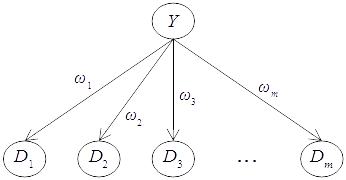
\includegraphics{MEDNetwork.png}
\caption{Diagnostic relationship with multiple evidences (M-E-D network)}
\label{figure:med-network}
\end{figure}
%Figure 4.3. Diagnostic relationship with multiple evidences (M-E-D network)

Figure~\ref{figure:med-network} depicts the multi-evidence diagnostic network called M-E-D network in which there are \textit{m} evidences \textit{D}${}_{1}$, \textit{D}${}_{2}$,{\dots}, \textit{D${}_{m}$} and one hypothesis \textit{Y}. Note that \textit{Y} has uniform distribution.

In simplest case where all evidences are binary, the joint probability of M-E-D network is:
\begin{align*}
P\left(Y,D_1,D_2,\dots ,D_m\right)&=P\left(Y\right)\prod^m_{j=1}{P\left(D_j\mathrel{\left|\vphantom{D_j Y}\right.\kern-\nulldelimiterspace}Y\right)}\\
&=P\left(Y\right)P\left(D_1,D_2,\dots ,D_m\mathrel{\left|\vphantom{D_1,D_2,\dots ,D_m Y}\right.\kern-\nulldelimiterspace}Y\right)
\end{align*}
The product $\prod^m_{j=1}{P\left(D_j\mathrel{\left|\vphantom{D_j Y}\right.\kern-\nulldelimiterspace}Y\right)}$ is denoted as likelihood function as follows:
\[P\left(D_1,D_2,\dots ,D_m\mathrel{\left|\vphantom{D_1,D_2,\dots ,D_m Y}\right.\kern-\nulldelimiterspace}Y\right)=\prod^m_{j=1}{P\left(D_j\mathrel{\left|\vphantom{D_j Y}\right.\kern-\nulldelimiterspace}Y\right)}\] 
The posterior probability \textit{P}(\textit{Y} {\textbar} \textit{D}${}_{1}$, \textit{D}${}_{2}$,{\dots}, \textit{D${}_{m}$}) given uniform distribution of \textit{Y} is:
\begin{align*}
&P\left(Y\mathrel{\left|\vphantom{Y D_1,D_2,\dots ,D_m}\right.\kern-\nulldelimiterspace}D_1,D_2,\dots ,D_m\right)\\
&=\frac{P\left(Y,D_1,D_2,\dots ,D_m\right)}{P\left(Y=1,D_1,D_2,\dots ,D_m\right)+P\left(Y=0,D_1,D_2,\dots ,D_m\right)}\\
&=\frac{1}{\prod^m_{j=1}{P\left(D_j\mathrel{\left|\vphantom{D_j Y=1}\right.\kern-\nulldelimiterspace}Y=1\right)}+\prod^m_{j=1}{P\left(D_j\mathrel{\left|\vphantom{D_j Y=0}\right.\kern-\nulldelimiterspace}Y=0\right)}}*P\left(D_1,D_2,\dots ,D_m\mathrel{\left|\vphantom{D_1,D_2,\dots ,D_m Y}\right.\kern-\nulldelimiterspace}Y\right)
\end{align*}
The possible transformation coefficient is:
\[\frac{1}{k}=\prod^m_{j=1}{P\left(D_j\mathrel{\left|\vphantom{D_j Y=1}\right.\kern-\nulldelimiterspace}Y=1\right)}+\prod^m_{j=1}{P\left(D_j\mathrel{\left|\vphantom{D_j Y=0}\right.\kern-\nulldelimiterspace}Y=0\right)}\] 
M-E-D network will satisfy diagnostic condition if \textit{k} = 1 because all hypotheses and evidence are binary, which leads that following equation specified by formula~\ref{formula:diagnostic-cond-med-network} has 2\textit{m} real roots \textit{P}(\textit{D${}_{j}${\textbar}Y}) for all \textit{m} $\mathrm{\ge}$ 2.

\begin{equation}
\prod^m_{j=1}{P\left(D_j\mathrel{\left|\vphantom{D_j Y=1}\right.\kern-\nulldelimiterspace}Y=1\right)}+\prod^m_{j=1}{P\left(D_j\mathrel{\left|\vphantom{D_j Y=0}\right.\kern-\nulldelimiterspace}Y=0\right)}=1
\label{formula:diagnostic-cond-med-network}
\end{equation}
%Formula 4.11. Diagnostic condition equation of binary M-E-D network 

The equation~\ref{formula:diagnostic-cond-med-network} has no real root given \textit{m}=2 according to following proof. Suppose equation~\ref{formula:diagnostic-cond-med-network} has 4 real roots as follows:
\begin{align*}
&a_1=P\left(D_1=1\mathrel{\left|\vphantom{D_1=1 Y=1}\right.\kern-\nulldelimiterspace}Y=1\right)\\
&a_2=P\left(D_2=1\mathrel{\left|\vphantom{D_2=1 Y=1}\right.\kern-\nulldelimiterspace}Y=1\right)\\
&b_1=P\left(D_1=1\mathrel{\left|\vphantom{D_1=1 Y=0}\right.\kern-\nulldelimiterspace}Y=0\right)\\
&b_2=P\left(D_2=1\mathrel{\left|\vphantom{D_2=1 Y=0}\right.\kern-\nulldelimiterspace}Y=0\right)
\end{align*}
From equation~\ref{formula:diagnostic-cond-med-network}, it holds:
\begin{align*}
&\left\{ \begin{array}{l}
a_1a_2+b_1b_2=1 \\ 
a_1\left(1-a_2\right)+b_1b_2=1 \\ 
\left(1-a_1\right)a_2+b_1b_2=1 \\ 
a_1a_2+b_1\left(1-b_2\right)=1 \\ 
a_1a_2+\left(1-b_1\right)b_2=1 \end{array}
\right.\Rightarrow \left\{ \begin{array}{l}
a_1=a_2 \\ 
b_1=b_2 \\ 
a^2_1+b^2_1=1 \\ 
a_1+2b^2_1=2 \\ 
b_1+2a^2_1=2 \end{array}
\right.\\
&\Leftrightarrow \left\{ \begin{array}{l}
a_1=a_2=0 \\ 
b_1=b_2 \\ 
a^2_1+b^2_1=1 \\ 
b_1=2 \end{array}
\right.\ \mathrm{or}\ \left\{ \begin{array}{l}
a_1=a_2=0.5 \\ 
b_1=b_2 \\ 
a^2_1+b^2_1=1 \\ 
b_1=1.5 \end{array}
\right.
\end{align*}
The final equation leads a contradiction (\textit{b}${}_{1}$=2 or \textit{b}${}_{1}$=1.5) and so it is impossible to apply the sufficient diagnostic proposition into M-E-D network. Such proposition is only used for one-evidence network. Moreover, X-gate inference absorbs many sources and then produces out of one targeted result whereas the M-E-D network essentially splits one source into many results. It is impossible to model M-E-D network by X-gates. The potential solution for this problem is to group many evidences \textit{D}${}_{1}$, \textit{D}${}_{2}$,{\dots}, \textit{D${}_{m}$} into one representative evidence \textit{D} which in turn is dependent on hypothesis \textit{Y} but this solution will be inaccurate in specifying conditional probabilities because directions of dependencies become inconsistent (relationships from \textit{D${}_{j}$} to \textit{D} and from \textit{Y} to \textit{D}) except that all \textit{D${}_{j}$} (s) are removed and \textit{D} becomes a vector. However evidence vector does not simplify the hazardous problem and it changes the current problem into a new problem.

Another solution is to reverse the direction of relationship, in which the hypothesis is dependent on evidences so as to take advantages of X-gate inference as usual. However, the reversion method violates the viewpoint in this research where diagnostic relationship must be from hypothesis to evidence. In other words, we should change the viewpoint.

Another solution is based on a so-called \textit{partial diagnostic condition} that is a loose case of diagnostic condition for M-E-D network, which is defined as follows:
\[P\left(Y\mathrel{\left|\vphantom{Y D_j}\right.\kern-\nulldelimiterspace}D_j\right)=kP\left(D_j\mathrel{\left|\vphantom{D_j Y}\right.\kern-\nulldelimiterspace}Y\right)\] 
Where \textit{k} is constant with regard to \textit{D${}_{j}$}. The joint probability is:
\[P\left(Y,D_1,D_2,\dots ,D_m\right)=P\left(Y\right)\prod^m_{j=1}{P\left(D_j\mathrel{\left|\vphantom{D_j Y}\right.\kern-\nulldelimiterspace}Y\right)}\] 
M-E-D network satisfies partial diagnostic condition. In fact, given all variables are binary, we have:
\begin{align*}
&P\left(Y\mathrel{\left|\vphantom{Y D_j}\right.\kern-\nulldelimiterspace}D_j\right)=\frac{\sum_{\mathrm{\Psi }\backslash \left\{Y,D_j\right\}}{P\left(Y,D_1,D_2,\dots ,D_m\right)}}{\sum_{\mathrm{\Psi }\backslash \left\{D_j\right\}}{P\left(Y,D_1,D_2,\dots ,D_m\right)}}\\
&\left(\mathrm{Let}\ \Psi=\left\{D_1,D_2,\dots,D_m\right\}\right)\\
&=\frac{P\left(D_j\mathrel{\left|\vphantom{D_j Y}\right.\kern-\nulldelimiterspace}Y\right)\prod^m_{k=1,k\neq j}{\left(\sum_{D_k}{P\left(D_k\mathrel{\left|\vphantom{D_k Y}\right.\kern-\nulldelimiterspace}Y\right)}\right)}}{\prod^m_{k=1,k\neq j}{\left(\sum_{D_k}{P\left(D_k\mathrel{\left|\vphantom{D_k Y=1}\right.\kern-\nulldelimiterspace}Y=1\right)}\right)}+\prod^m_{k=1,k\neq j}{\left(\sum_{D_k}{P\left(D_k\mathrel{\left|\vphantom{D_k Y=0}\right.\kern-\nulldelimiterspace}Y=0\right)}\right)}}\\
&\left(\mathrm{Due}\ \mathrm{to}\ \mathrm{uniform}\ \mathrm{distribution}\ \mathrm{of}\ Y\right)\\
&=\frac{P\left(D_j\mathrel{\left|\vphantom{D_j Y}\right.\kern-\nulldelimiterspace}Y\right)\prod^m_{k=1,k\neq j}{1}}{\prod^m_{k=1,k\neq j}{1}+\prod^m_{k=1,k\neq j}{1}}=\frac{1}{2}P\left(D_j\mathrel{\left|\vphantom{D_j Y}\right.\kern-\nulldelimiterspace}Y\right)\\
&\left(\mathrm{Due\ to}\ \sum_{D_k}{P\left(D_k\mathrel{\left|\vphantom{D_k Y}\right.\kern-\nulldelimiterspace}Y\right)}=P\left(D_k=0\mathrel{\left|\vphantom{D_k=0 Y}\right.\kern-\nulldelimiterspace}Y\right)+P\left(D_k=1\mathrel{\left|\vphantom{D_k=1 Y}\right.\kern-\nulldelimiterspace}Y\right)=1\right)
\end{align*}
Partial diagnostic condition expresses a different viewpoint. It is not an optimal solution because we cannot test a disease based on only one symptom while ignoring other obvious symptoms, for example. The equality \textit{P}(\textit{Y{\textbar}D${}_{j}$}) = 0.5\textit{P}(\textit{D${}_{j}${\textbar}Y}) indicates the accuracy is decreased two times. However, Bayesian network provides inference mechanism based on personal belief. It is subjective. You can use partial diagnostic condition if you think that such condition is appropriate to your application.

If we are successful in specifying conditional probabilities of M-E-D network, it is possible to define an extended network which is constituted of \textit{n} hypotheses \textit{X}${}_{1}$, \textit{X}${}_{2}$,{\dots}, \textit{X${}_{n}$} and \textit{m} evidences \textit{D}${}_{1}$, \textit{D}${}_{2}$,{\dots}, \textit{D${}_{m}$}. Such extended network represents \textit{multi-hypothesis multi-evidence diagnostic relationship}, called M-HE-D network. Figure~\ref{figure:mhed-network} depicts M-HE-D network.

\begin{figure}
\centering
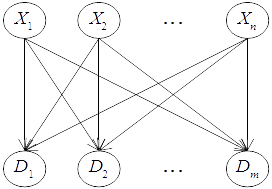
\includegraphics{MHEDNetwork.png}
\caption{M-HE-D network}
\label{figure:mhed-network}
\end{figure}
%Figure 5.1. M-HE-D network

The M-HE-D network is the most general case of diagnostic network, which was mentioned in \cite{millan:bayesiandiagnostic}. We can construct any large diagnostic BN from M-HE-D networks and so the research is still open.

\section{Conclusion}
In short, relationship conversion is to determine conditional probabilities based on logic gates that is adhered to semantics of relationships. The weak point of logic gates is to require that all variables must be binary. For example, in learning context, it is inconvenient for expert to create an assessment BN with studying exercises (evidences) whose marks are only 0 and 1. In order to lessen the impact of such weak point, I use numeric evidence for extending capacity of simple Bayesian network. However, combination of binary hypothesis and numeric evidence leads to errors or biases in inference. For example, given a student gets maximum grade for an exercise but the built-in inference results out that she/he has not mastered fully the associated learning concept (hypothesis). Therefore, I propose the sufficient diagnostic proposition so as to confirm that numeric evidence is adequate to make complicated inference tasks in BN. The probabilistic reasoning based on evidence is always accurate. Application of the research can go beyond learning context whenever probabilistic deduction relevant to constraints of semantic relationships is required. A large BN can be constituted of many simple BN (s). Inference in large BN is hazardous problem and there are many optimal algorithms for solving such problem. In future, I will research effective inference methods for the special BN that is constituted of X-gate BN (s) mentioned in this research because X-gate BN (s) have precise and useful features of which we should take advantages. For instance, their CPT (s) are simple in some cases and the meanings of their relationships are mandatory in many applications. Moreover, I try my best to research deeply M-E-D network and M-HE-D network whose problems I cannot solve absolutely now.

Two main documents I referred to do this research are the book ``Learning Bayesian Networks'' \cite{neapolitan:bn} by the author Richard E. Neapolitan and the article ``A Bayesian Diagnostic Algorithm for Student Modeling and its Evaluation'' \cite{millan:bayesiandiagnostic} by authors Eva Millán and José Luis Pérez-de-la-Cruz. Especially, the SIGMA-gate inference is based on and derived from the work of the authors Eva Millán and José Luis Pérez-de-la-Cruz. This research is originated from my PhD research ``A User Modeling System for Adaptive Learning'' \cite{nguyen:zebra}. Other references relevant to user modeling, overlay model, and Bayesian network are \cite{froschl:usermodeling}, \cite{debra:aha}, \cite{murphy:bn}, and \cite{heckerman:bn}. Please concern these references.

\bibliographystyle{abbrv}
\bibliography{RelationshipConversionBN}

\end{document}

